% Options for packages loaded elsewhere
\PassOptionsToPackage{unicode}{hyperref}
\PassOptionsToPackage{hyphens}{url}
\documentclass[
]{book}
\usepackage{xcolor}
\usepackage{amsmath,amssymb}
\setcounter{secnumdepth}{5}
\usepackage{iftex}
\ifPDFTeX
  \usepackage[T1]{fontenc}
  \usepackage[utf8]{inputenc}
  \usepackage{textcomp} % provide euro and other symbols
\else % if luatex or xetex
  \usepackage{unicode-math} % this also loads fontspec
  \defaultfontfeatures{Scale=MatchLowercase}
  \defaultfontfeatures[\rmfamily]{Ligatures=TeX,Scale=1}
\fi
\usepackage{lmodern}
\ifPDFTeX\else
  % xetex/luatex font selection
\fi
% Use upquote if available, for straight quotes in verbatim environments
\IfFileExists{upquote.sty}{\usepackage{upquote}}{}
\IfFileExists{microtype.sty}{% use microtype if available
  \usepackage[]{microtype}
  \UseMicrotypeSet[protrusion]{basicmath} % disable protrusion for tt fonts
}{}
\makeatletter
\@ifundefined{KOMAClassName}{% if non-KOMA class
  \IfFileExists{parskip.sty}{%
    \usepackage{parskip}
  }{% else
    \setlength{\parindent}{0pt}
    \setlength{\parskip}{6pt plus 2pt minus 1pt}}
}{% if KOMA class
  \KOMAoptions{parskip=half}}
\makeatother
\usepackage{color}
\usepackage{fancyvrb}
\newcommand{\VerbBar}{|}
\newcommand{\VERB}{\Verb[commandchars=\\\{\}]}
\DefineVerbatimEnvironment{Highlighting}{Verbatim}{commandchars=\\\{\}}
% Add ',fontsize=\small' for more characters per line
\usepackage{framed}
\definecolor{shadecolor}{RGB}{248,248,248}
\newenvironment{Shaded}{\begin{snugshade}}{\end{snugshade}}
\newcommand{\AlertTok}[1]{\textcolor[rgb]{0.94,0.16,0.16}{#1}}
\newcommand{\AnnotationTok}[1]{\textcolor[rgb]{0.56,0.35,0.01}{\textbf{\textit{#1}}}}
\newcommand{\AttributeTok}[1]{\textcolor[rgb]{0.13,0.29,0.53}{#1}}
\newcommand{\BaseNTok}[1]{\textcolor[rgb]{0.00,0.00,0.81}{#1}}
\newcommand{\BuiltInTok}[1]{#1}
\newcommand{\CharTok}[1]{\textcolor[rgb]{0.31,0.60,0.02}{#1}}
\newcommand{\CommentTok}[1]{\textcolor[rgb]{0.56,0.35,0.01}{\textit{#1}}}
\newcommand{\CommentVarTok}[1]{\textcolor[rgb]{0.56,0.35,0.01}{\textbf{\textit{#1}}}}
\newcommand{\ConstantTok}[1]{\textcolor[rgb]{0.56,0.35,0.01}{#1}}
\newcommand{\ControlFlowTok}[1]{\textcolor[rgb]{0.13,0.29,0.53}{\textbf{#1}}}
\newcommand{\DataTypeTok}[1]{\textcolor[rgb]{0.13,0.29,0.53}{#1}}
\newcommand{\DecValTok}[1]{\textcolor[rgb]{0.00,0.00,0.81}{#1}}
\newcommand{\DocumentationTok}[1]{\textcolor[rgb]{0.56,0.35,0.01}{\textbf{\textit{#1}}}}
\newcommand{\ErrorTok}[1]{\textcolor[rgb]{0.64,0.00,0.00}{\textbf{#1}}}
\newcommand{\ExtensionTok}[1]{#1}
\newcommand{\FloatTok}[1]{\textcolor[rgb]{0.00,0.00,0.81}{#1}}
\newcommand{\FunctionTok}[1]{\textcolor[rgb]{0.13,0.29,0.53}{\textbf{#1}}}
\newcommand{\ImportTok}[1]{#1}
\newcommand{\InformationTok}[1]{\textcolor[rgb]{0.56,0.35,0.01}{\textbf{\textit{#1}}}}
\newcommand{\KeywordTok}[1]{\textcolor[rgb]{0.13,0.29,0.53}{\textbf{#1}}}
\newcommand{\NormalTok}[1]{#1}
\newcommand{\OperatorTok}[1]{\textcolor[rgb]{0.81,0.36,0.00}{\textbf{#1}}}
\newcommand{\OtherTok}[1]{\textcolor[rgb]{0.56,0.35,0.01}{#1}}
\newcommand{\PreprocessorTok}[1]{\textcolor[rgb]{0.56,0.35,0.01}{\textit{#1}}}
\newcommand{\RegionMarkerTok}[1]{#1}
\newcommand{\SpecialCharTok}[1]{\textcolor[rgb]{0.81,0.36,0.00}{\textbf{#1}}}
\newcommand{\SpecialStringTok}[1]{\textcolor[rgb]{0.31,0.60,0.02}{#1}}
\newcommand{\StringTok}[1]{\textcolor[rgb]{0.31,0.60,0.02}{#1}}
\newcommand{\VariableTok}[1]{\textcolor[rgb]{0.00,0.00,0.00}{#1}}
\newcommand{\VerbatimStringTok}[1]{\textcolor[rgb]{0.31,0.60,0.02}{#1}}
\newcommand{\WarningTok}[1]{\textcolor[rgb]{0.56,0.35,0.01}{\textbf{\textit{#1}}}}
\usepackage{longtable,booktabs,array}
\usepackage{calc} % for calculating minipage widths
% Correct order of tables after \paragraph or \subparagraph
\usepackage{etoolbox}
\makeatletter
\patchcmd\longtable{\par}{\if@noskipsec\mbox{}\fi\par}{}{}
\makeatother
% Allow footnotes in longtable head/foot
\IfFileExists{footnotehyper.sty}{\usepackage{footnotehyper}}{\usepackage{footnote}}
\makesavenoteenv{longtable}
\usepackage{graphicx}
\makeatletter
\newsavebox\pandoc@box
\newcommand*\pandocbounded[1]{% scales image to fit in text height/width
  \sbox\pandoc@box{#1}%
  \Gscale@div\@tempa{\textheight}{\dimexpr\ht\pandoc@box+\dp\pandoc@box\relax}%
  \Gscale@div\@tempb{\linewidth}{\wd\pandoc@box}%
  \ifdim\@tempb\p@<\@tempa\p@\let\@tempa\@tempb\fi% select the smaller of both
  \ifdim\@tempa\p@<\p@\scalebox{\@tempa}{\usebox\pandoc@box}%
  \else\usebox{\pandoc@box}%
  \fi%
}
% Set default figure placement to htbp
\def\fps@figure{htbp}
\makeatother
\setlength{\emergencystretch}{3em} % prevent overfull lines
\providecommand{\tightlist}{%
  \setlength{\itemsep}{0pt}\setlength{\parskip}{0pt}}
\usepackage[]{natbib}
\bibliographystyle{plainnat}
\usepackage{booktabs}
\AtBeginDocument{\renewcommand{\chaptername}{Kapitel}}

\usepackage[swedish]{babel}
\selectlanguage{swedish}
\usepackage{booktabs}
\usepackage{longtable}
\usepackage{array}
\usepackage{multirow}
\usepackage{wrapfig}
\usepackage{float}
\usepackage{colortbl}
\usepackage{pdflscape}
\usepackage{tabu}
\usepackage{threeparttable}
\usepackage{threeparttablex}
\usepackage[normalem]{ulem}
\usepackage{makecell}
\usepackage{xcolor}
\usepackage{bookmark}
\IfFileExists{xurl.sty}{\usepackage{xurl}}{} % add URL line breaks if available
\urlstyle{same}
\hypersetup{
  pdftitle={R-anvisningar till Grundläggande statistik},
  hidelinks,
  pdfcreator={LaTeX via pandoc}}

\title{R-anvisningar till \emph{Grundläggande statistik}}
\author{}
\date{\vspace{-2.5em}2025-09-19}

\usepackage{amsthm}
\newtheorem{theorem}{Sats}[chapter]
\newtheorem{lemma}{Lemma}[chapter]
\newtheorem{corollary}{Corollary}[chapter]
\newtheorem{proposition}{Problem}[chapter]
\newtheorem{conjecture}{Conjecture}[chapter]
\theoremstyle{definition}
\newtheorem{definition}{Definition}[chapter]
\theoremstyle{definition}
\newtheorem{example}{Exempel}[chapter]
\theoremstyle{definition}
\newtheorem{exercise}{Uppgift}[chapter]
\theoremstyle{definition}
\newtheorem{hypothesis}{Lösningsförslag}[chapter]
\theoremstyle{remark}
\newtheorem*{remark}{Remark}
\newtheorem*{solution}{Solution}
\begin{document}
\maketitle

{
\setcounter{tocdepth}{1}
\tableofcontents
}
\chapter*{Introduktion}\label{introduktion}
\addcontentsline{toc}{chapter}{Introduktion}

Detta dokument ger en introduktion till R för en kurs i grundläggande statistik.

\chapter*{Installation av R och RStudio}\label{installation-av-r-och-rstudio}
\addcontentsline{toc}{chapter}{Installation av R och RStudio}

\section{Inledning}\label{inledning}

För att köra R-kod på sin dator krävs en installation av programspråket R. För att effektivt arbeta i R används ofta en utvecklingsmiljö (ett tilläggsprogram som på flera sätt förenklar arbetet) och här ges anvisningar till RStudio - den vanligaste utvecklingsmiljön för R. För att komma ingång måste man alltså installera R och RStudio.

\section{Installation av R}\label{installation-av-r}

Programspråket R kan laddas ner från \url{https://www.r-project.org/} med följande steg:

\begin{enumerate}
\def\labelenumi{\arabic{enumi}.}
\tightlist
\item
  Klicka på \emph{CRAN} längst upp till vänster.
\item
  Klicka på den översta länken under 0-Cloud.
\item
  Välj en nedladdning beroende på operativsystem.
\item
  För Windows, välj \emph{base}. För macOS, välj den senaste tillgängliga versionen.
\item
  Installera R från den nedladdade filen. Installation sker som för andra nedladdade program.
\end{enumerate}

\section{Installation av RStudio}\label{installation-av-rstudio}

RStudio kan laddas ner från \url{https://www.posit.co/} med följande steg:

\begin{enumerate}
\def\labelenumi{\arabic{enumi}.}
\tightlist
\item
  Klicka på \emph{Download RStudio} uppe till höger.
\item
  Scrolla nedåt och välj \emph{Download} under \emph{Install RStudio}.
\item
  Installera RStudio från den nedladdade filen. Installation sker som för andra nedladdade program.
\end{enumerate}

\section{Gränssnittet i RStudio}\label{gruxe4nssnittet-i-rstudio}

När man nu öppnar RStudio ser man att fönstret är uppdelat i fyra delar och att varje del består av en eller flera flikar. De viktigaste är i nuläget

\begin{itemize}
\tightlist
\item
  \emph{Console} där kod körs och resultat skrivs ut,
\item
  \emph{Environment} där man ser skapade objekt,
\item
  \emph{History} där man ser tidigare körd kod,
\item
  \emph{Plots} där man ser skapade grafer, och
\item
  \emph{Help} där man ser hjälpsidor för funktioner.
\end{itemize}

Ofta skriver man inte sin kod direkt i konsollen, utan i ett separat \emph{skript} - en vanlig textfil som innehåller den kod man vill köra. Genom att organisera sin kod i ett skript kan man lätt strukturera och dokumentera sitt arbete. I RStudio kan man öppna ett nytt skript genom att gå till \emph{File \textgreater{} New File \textgreater{} R Script} eller genom att klicka \emph{Ctrl + Shift + N}. Ett tomt skript öppnar sig då i det övre vänstra delfönstret. Om man skriver

\begin{Shaded}
\begin{Highlighting}[]
\NormalTok{a }\OtherTok{\textless{}{-}} \DecValTok{5}
\end{Highlighting}
\end{Shaded}

i skriptet och trycker \emph{Ctrl + Enter} bör man se att koden i skriptet körs i konsollen. Om man tittar i fliken \emph{Environment} ska man också se att det nu skapats ett objekt \emph{a}.

\section{Paket i R}\label{paket-i-r}

En av de stora styrkorna med R är att språket kan byggas ut av dess användare. De här tilläggen kan sedan samlas i paket (\emph{packages}) och delas med andra. Rs officiella bibliotek för paket kallas för \emph{CRAN} (\emph{Comprehensive R Archive Network}) och består av drygt 20 000 uppladdade paket som innehåller allt från fritt tillgänglig data till avancerade statistiska modeller.

För att använda ett specifikt paket måste det först installeras. Om man vet namnet på paketet man vill installera kan man köra

\begin{Shaded}
\begin{Highlighting}[]
\FunctionTok{install.packages}\NormalTok{(}\StringTok{"tidyverse"}\NormalTok{)}
\end{Highlighting}
\end{Shaded}

I det här fallet installeras paketet \texttt{tidyverse}, vilket innehåller funktioner för hantering av data.

I RStudio kan man också installera paket från \emph{Packages}-fliken.

Paket måste också laddas för varje ny session. Innan man kan använda innehållet i ett paket måste man därför köra

\begin{Shaded}
\begin{Highlighting}[]
\FunctionTok{library}\NormalTok{(tidyverse)}
\end{Highlighting}
\end{Shaded}

\chapter{Datahantering och grafer}\label{datahantering-och-grafer}

Datorövning 1 handlar om grunderna till R. Efter övningen ska vi kunna

\begin{itemize}
\tightlist
\item
  Starta RStudio och orientera oss i gränssnittet,
\item
  Installera och ladda tilläggspaket (\emph{Packages}),
\item
  Definera objekt och tillämpa funktioner i R,
\item
  Transformera en tabell med data genom att välja kolumner och filtrera rader,
\item
  Skapa grafer med \texttt{ggplot2}.
\end{itemize}

\section{Uppstart och orientering}\label{uppstart-och-orientering}

För att arbeta i R måste vi installera språket R och ett gränssnitt för att arbeta i R, vanligen \emph{RStudio}. Både R och RStudio kan laddas ner gratis, från \url{https://www.r-project.org/} respektive \url{https://posit.co/}.

Starta RStudio, till exempel genom att gå till Startmenyn och söka på RStudio eller genom att dubbelklicka på en fil som öppnas i RStudio.
Gränssnittet i RStudio är uppdelat i fyra delar och varje del består av en eller flera flikar. De viktigaste är i nuläget

\begin{itemize}
\tightlist
\item
  \emph{Console} där kod körs och resultat skrivs ut,
\item
  \emph{Environment} där man ser skapade objekt,
\item
  \emph{History} där man ser tidigare körd kod,
\item
  \emph{Plots} där man ser skapade grafer, och
\item
  \emph{Help} där man ser hjälpsidor för funktioner.
\end{itemize}

\begin{exercise}[Help-fliken]
Hitta fliken \emph{Help}, klicka på husikonen under fliken. Finns det en länk med \emph{RStudio Cheat Sheets}? Följ den länken för att hitta guider till R som kan bli nyttiga längre fram. För nu, gå tillbaka till RStudio.
\end{exercise}

Ofta skriver man inte sin kod direkt i konsollen, utan i ett separat \emph{skript} - en vanlig textfil som innehåller den kod man vill köra. I RStudio kan man öppna ett nytt skript genom att gå till \emph{File \textgreater{} New File \textgreater{} R Script} eller genom att klicka \emph{Ctrl + Shift + N}.

\begin{exercise}[Ett första skript]
Öppna ett nytt skript genom File-menyn eller genom \emph{Ctrl + Shift + N}.
Skriv

\begin{Shaded}
\begin{Highlighting}[]
\NormalTok{a }\OtherTok{\textless{}{-}} \DecValTok{5}
\end{Highlighting}
\end{Shaded}

i skriptet och tryck \emph{Ctrl + Enter}. Titta i flikarna \emph{Console} och \emph{Environment}. Har något hänt? Du bör se att koden i skriptet körts i konsollen och att ett nytt objekt \texttt{a} ligger i \emph{Environment}.
\end{exercise}

\section{\texorpdfstring{\emph{Packages} från CRAN}{Packages från CRAN}}\label{packages-fruxe5n-cran}

En av de stora styrkorna med R är att språket kan byggas ut av dess användare. De här tilläggen kan sedan samlas i paket (\emph{packages}) och delas med andra. Rs officiella bibliotek för paket kallas för \emph{CRAN} (\emph{Comprehensive R Archive Network}).

För att använda ett specifikt paket måste det först installeras. Om man vet namnet på paketet man vill installera kan man köra

\begin{Shaded}
\begin{Highlighting}[]
\FunctionTok{install.packages}\NormalTok{(}\StringTok{"tidyverse"}\NormalTok{)}
\end{Highlighting}
\end{Shaded}

I det här fallet installeras paketet \texttt{tidyverse}, vilket innehåller funktioner för hantering av data.

I RStudio kan man också installera paket från \emph{Packages}-fliken.

\begin{exercise}[Installera tidyverse-paketet]
Kör raden ovan för att installera \texttt{tidyverse}. Du kan antingen köra raden genom att skriva den i \emph{Console} eller genom att skriva i ett skript och köra därifrån genom \emph{Ctrl + Enter}.
\end{exercise}

\begin{exercise}[Installera gapminder-paketet]

Paketet \texttt{gapminder} innehåller lite intressant data vi kommer använda senare. Installera paketet \texttt{gapminder} genom att fylla i den saknade biten och köra raden nedan.

\begin{Shaded}
\begin{Highlighting}[]
\FunctionTok{install.packages}\NormalTok{(}\StringTok{"\_\_\_"}\NormalTok{)}
\end{Highlighting}
\end{Shaded}

\end{exercise}

Paket måste också laddas för varje ny session. Innan man kan använda innehållet i ett paket måste man därför köra

\begin{Shaded}
\begin{Highlighting}[]
\FunctionTok{library}\NormalTok{(tidyverse)}
\end{Highlighting}
\end{Shaded}

\begin{exercise}[Ladda gapminder-paketet]

Ladda paketet \texttt{gapminder} genom att fylla i och köra raden nedan.

\begin{Shaded}
\begin{Highlighting}[]
\FunctionTok{library}\NormalTok{(\_\_\_)}
\end{Highlighting}
\end{Shaded}

\end{exercise}

\begin{exercise}[Paket som inte finns]

Vad händer om man försöker installera ett paket som inte finns på \emph{CRAN}? Testa till exempel

\begin{Shaded}
\begin{Highlighting}[]
\FunctionTok{install.packages}\NormalTok{(}\StringTok{"ThisIsNotTheNameOfAnyPackage"}\NormalTok{)}
\end{Highlighting}
\end{Shaded}

och

\begin{Shaded}
\begin{Highlighting}[]
\FunctionTok{library}\NormalTok{(ThisIsNotTheNameOfAnyPackage)}
\end{Highlighting}
\end{Shaded}

\end{exercise}

\section{Objekt och funktioner}\label{objekt-och-funktioner}

Ett \emph{objekt} i R är en namngiven informationsmängd. Objekt kan se ut på många olika sätt - under kursens gång används objekt som består av insamlad data (konstruerade som vektorer eller tabeller), objekt som är statistiska modeller, och flera andra former. I R skapar man objekt med \emph{assign}-pilen \texttt{\textless{}-} (mindre än och bindestreck).

I ett tidigare exempel fanns raden

\begin{Shaded}
\begin{Highlighting}[]
\NormalTok{a }\OtherTok{\textless{}{-}} \DecValTok{5}
\end{Highlighting}
\end{Shaded}

Här skapas ett objekt med namnet \texttt{a} som innehåller informationen \texttt{5}. \emph{Assign}-pilen pekar alltså på det namn man vill ge objektet och pekar från objektets innehåll.

Ett lite mer komplicerat exempel på ett objekt ges av

\begin{Shaded}
\begin{Highlighting}[]
\NormalTok{b }\OtherTok{\textless{}{-}} \FunctionTok{c}\NormalTok{(}\DecValTok{3}\NormalTok{, }\DecValTok{1}\NormalTok{, }\DecValTok{4}\NormalTok{, }\DecValTok{1}\NormalTok{, }\DecValTok{5}\NormalTok{, }\DecValTok{9}\NormalTok{)}
\end{Highlighting}
\end{Shaded}

Här skapas ett objekt \texttt{b} som innehåller en \emph{serie} numeriska värden (en \emph{vektor}). Värdena i en vektor är ordnade och man kan plocka ut ett specifikt värde med hakparenteser.

\begin{Shaded}
\begin{Highlighting}[]
\NormalTok{b[}\DecValTok{3}\NormalTok{]               }\CommentTok{\# Det tredje värdet i vektorn b}
\end{Highlighting}
\end{Shaded}

\begin{verbatim}
## [1] 4
\end{verbatim}

\begin{Shaded}
\begin{Highlighting}[]
\NormalTok{b[}\FunctionTok{c}\NormalTok{(}\DecValTok{3}\NormalTok{,}\DecValTok{5}\NormalTok{)]          }\CommentTok{\# Det tredje och femte värdet i b}
\end{Highlighting}
\end{Shaded}

\begin{verbatim}
## [1] 4 5
\end{verbatim}

\begin{exercise}[Skapa en vektor]

Skapa ett objekt med namnet \texttt{new\_vector} som innehåller värden 5, 7 och 10 genom att fylla i följande rad.

\begin{Shaded}
\begin{Highlighting}[]
\NormalTok{new\_vector }\OtherTok{\textless{}{-}} \FunctionTok{c}\NormalTok{(\_, \_, \_)}
\end{Highlighting}
\end{Shaded}

\end{exercise}

\begin{exercise}[Ta ut andra värdet]
Använd hakparenteser för att plocka ut det andra värdet ur vektorn \texttt{new\_vector}.
\end{exercise}

Objekt kan manipuleras genom att tillämpa \emph{funktioner}. En funktion tar någon ingående data och ger något utgående resultat. Funktioner anges genom att skriva funktionens namn följt av ingående data inom parenteser, och resultatet kan antingen skrivas ut i konsollen eller sparas som ett nytt objekt. En grundinstallation av R innehåller en mängd färdiga funktioner, t.ex.

\begin{Shaded}
\begin{Highlighting}[]
\FunctionTok{sum}\NormalTok{(b)}
\end{Highlighting}
\end{Shaded}

\begin{verbatim}
## [1] 23
\end{verbatim}

vilket ger summan av värdena i vektorn \texttt{b},

\begin{Shaded}
\begin{Highlighting}[]
\FunctionTok{plot}\NormalTok{(b)}
\end{Highlighting}
\end{Shaded}

som ger en simpel graf, och

\begin{Shaded}
\begin{Highlighting}[]
\FunctionTok{sqrt}\NormalTok{(b)}
\end{Highlighting}
\end{Shaded}

\begin{verbatim}
## [1] 1.732051 1.000000 2.000000 1.000000 2.236068 3.000000
\end{verbatim}

som beräknar kvadratroten för varje element i vektorn.

\begin{exercise}[Summera vektorn]

Fyll i och kör följande rad för att beräkna summan av vektorn \texttt{new\_vector}

\begin{Shaded}
\begin{Highlighting}[]
\FunctionTok{sum}\NormalTok{(\_\_\_)}
\end{Highlighting}
\end{Shaded}

\end{exercise}

Vid konstruktionen av vektorn användes också en grundläggande funktion - funktionen \texttt{c()}, som tar en serie värden och skapar en sammanhängande vektor av värden.

Alla R-funktioner har en tillhörande hjälpfil som kan plockas fram genom att skriva frågetecken följt av funktionsnamnet, t.ex. \texttt{?sum}. Från hjälpfilen får man att \texttt{sum()} tar numeriska vektorer som ingående värde och beräknar summan. Man kan styra funktionens beteende genom att sätta ett argument \texttt{na.rm} (vilket här styr hur funktionen hanterar saknade värden). Som illustration kan man titta på

\begin{Shaded}
\begin{Highlighting}[]
\NormalTok{b }\OtherTok{\textless{}{-}} \FunctionTok{c}\NormalTok{(}\DecValTok{3}\NormalTok{, }\DecValTok{1}\NormalTok{, }\DecValTok{4}\NormalTok{, }\DecValTok{1}\NormalTok{, }\DecValTok{5}\NormalTok{, }\DecValTok{9}\NormalTok{, }\ConstantTok{NA}\NormalTok{)  }\CommentTok{\# Lägger till ett saknat värde}
\FunctionTok{sum}\NormalTok{(b)                        }\CommentTok{\# na.rm = FALSE är grundinställning}
\end{Highlighting}
\end{Shaded}

\begin{verbatim}
## [1] NA
\end{verbatim}

\begin{Shaded}
\begin{Highlighting}[]
\FunctionTok{sum}\NormalTok{(b, }\AttributeTok{na.rm =} \ConstantTok{TRUE}\NormalTok{)          }\CommentTok{\# na.rm sätts till TRUE}
\end{Highlighting}
\end{Shaded}

\begin{verbatim}
## [1] 23
\end{verbatim}

Det första försöket \texttt{sum(b)} ger utfallet \texttt{NA}, men om man sätter \texttt{na.rm\ =\ TRUE} beräknas summan efter att det saknade värdet plockats bort. Notera också att skript kan kommenteras med \texttt{\#}.

\section{Sekvenser av funktioner}\label{sekvenser-av-funktioner}

Ofta vill man genomföra flera operationer på ett objekt. Man behöver då genomföra en sekvens av funktioner. Säg till exempel att man har värdena \[(-4, -2, -1, 1, 2, 4)\] och vill ta absolutvärde (vilket gör negativa tal till motsvarande positiva tal) och sedan summera.
Den typen av sekvenser kan genomföras på ett par olika sätt. Ett första sätt är att spara resultatet i varje steg och sedan använda utfallet i nästa steg:

\begin{Shaded}
\begin{Highlighting}[]
\NormalTok{c }\OtherTok{\textless{}{-}} \FunctionTok{c}\NormalTok{(}\SpecialCharTok{{-}}\DecValTok{4}\NormalTok{, }\SpecialCharTok{{-}}\DecValTok{2}\NormalTok{, }\SpecialCharTok{{-}}\DecValTok{1}\NormalTok{, }\DecValTok{1}\NormalTok{, }\DecValTok{2}\NormalTok{, }\DecValTok{4}\NormalTok{)   }\CommentTok{\# Skapa en vektor av värden}
\NormalTok{c\_absolute }\OtherTok{\textless{}{-}} \FunctionTok{abs}\NormalTok{(c)          }\CommentTok{\# Ta absolutvärden. Skapa c\_absolut}
\FunctionTok{sum}\NormalTok{(c\_absolute)               }\CommentTok{\# Summera värden i c\_absolut}
\end{Highlighting}
\end{Shaded}

\begin{verbatim}
## [1] 14
\end{verbatim}

Här skapas ett objekt \texttt{c} som innehåller en vektor där några tal är negativa. I nästa rad används \texttt{abs} för att skapa absolutvärden. Slutligen summeras absolutvärdena med \texttt{sum}.
Notera att det är möjligt att skapa ett objekt med namnet \texttt{c} trots att det redan är namnet på en funktion - R förstår ur sammanhanget om objektet eller funktionen ska användas. Det kan dock bli lite oklart för en läsare, så försök som regel att undvika att skapa objekt med vanliga funktionsnamn som \texttt{sum} och \texttt{mean}.

\begin{exercise}[Kvadrat, summa och roten ur]

Fyll i och kör följande rader för att ta varje värde i \texttt{new\_vector} i kvadrat, \emph{sedan} summera, och sedan ta roten ur.

\begin{Shaded}
\begin{Highlighting}[]
\NormalTok{new\_vector\_squared }\OtherTok{\textless{}{-}}\NormalTok{ new\_vector}\SpecialCharTok{\^{}}\DecValTok{2} \CommentTok{\# Ta kvadraten av varje värde}
\NormalTok{new\_vector\_squared\_sum }\OtherTok{\textless{}{-}} \FunctionTok{sum}\NormalTok{(\_\_\_) }\CommentTok{\# Summera kvadraterna}
\FunctionTok{sqrt}\NormalTok{(\_\_\_)                          }\CommentTok{\# Ta kvadratroten ur summan}
\end{Highlighting}
\end{Shaded}

\end{exercise}

Ett alternativ till att spara utfallet i varje steg är att skriva en senare funktion \emph{runt} en tidigare funktion. Det fungerar för att R utvärderar funktioner inifrån-ut. Med samma exempel som tidigare får man

\begin{Shaded}
\begin{Highlighting}[]
\FunctionTok{sum}\NormalTok{(}\FunctionTok{abs}\NormalTok{(}\FunctionTok{c}\NormalTok{(}\SpecialCharTok{{-}}\DecValTok{4}\NormalTok{, }\SpecialCharTok{{-}}\DecValTok{2}\NormalTok{, }\SpecialCharTok{{-}}\DecValTok{1}\NormalTok{, }\DecValTok{1}\NormalTok{, }\DecValTok{2}\NormalTok{, }\DecValTok{4}\NormalTok{)))  }
\CommentTok{\# Ta summan av absolutvärden av vektorn}
\end{Highlighting}
\end{Shaded}

medan beräkningen i övningen blir

\begin{Shaded}
\begin{Highlighting}[]
\FunctionTok{sqrt}\NormalTok{(}\FunctionTok{sum}\NormalTok{(new\_vector}\SpecialCharTok{\^{}}\DecValTok{2}\NormalTok{)) }\CommentTok{\# Ta roten ur summan av vektorn i kvadrat}
\end{Highlighting}
\end{Shaded}

Den här typen av skrivning kan spara plats men blir snabbt svårläst.

Ett sista alternativ är att använda en så kallad \emph{pipe} (namnet kommer från att en sekvens funktioner kallas en \emph{pipeline}). En pipe skrivs \texttt{\%\textgreater{}\%} och kan i RStudio tas fram med kortkommandon \emph{Ctrl + Shift + M}. Pipen tar utfallet av en funktion till vänster och sänder till en funktion till höger. Den kan utläsas i dagligt tal som \emph{och sen}. Med samma exempel som tidigare kan vi skriva

\begin{Shaded}
\begin{Highlighting}[]
\FunctionTok{library}\NormalTok{(tidyverse)}

\FunctionTok{c}\NormalTok{(}\SpecialCharTok{{-}}\DecValTok{4}\NormalTok{, }\SpecialCharTok{{-}}\DecValTok{2}\NormalTok{, }\SpecialCharTok{{-}}\DecValTok{1}\NormalTok{, }\DecValTok{1}\NormalTok{, }\DecValTok{2}\NormalTok{, }\DecValTok{4}\NormalTok{) }\SpecialCharTok{\%\textgreater{}\%}        \CommentTok{\# Skapa en datamängd och sen}
  \FunctionTok{abs}\NormalTok{() }\SpecialCharTok{\%\textgreater{}\%}                       \CommentTok{\# ta absolutvärden, och sen}
  \FunctionTok{sum}\NormalTok{()                           }\CommentTok{\# beräkna summan.}
\end{Highlighting}
\end{Shaded}

\begin{verbatim}
## [1] 14
\end{verbatim}

\begin{exercise}[Kvadrat, summa och rot med pipe]

Fyll i de saknade funktionerna och kör följande rader för att ta varje värde i \texttt{new\_vector} i kvadrat, \emph{sedan} summera, och sedan ta roten ur, denna gång genom att länka funktionerna med en pipe \texttt{\%\textgreater{}\%}.

\begin{Shaded}
\begin{Highlighting}[]
\NormalTok{new\_vector}\SpecialCharTok{\^{}}\DecValTok{2} \SpecialCharTok{\%\textgreater{}\%} \CommentTok{\# Ta kvadraterna av new\_vector, och sen}
  \FunctionTok{\_\_\_}\NormalTok{() }\SpecialCharTok{\%\textgreater{}\%}      \CommentTok{\# beräkna summan, och sen}
  \FunctionTok{\_\_\_\_}\NormalTok{()         }\CommentTok{\# Ta kvadratroten med sqrt()}
\end{Highlighting}
\end{Shaded}

\end{exercise}

\section{Datainskrivning}\label{datainskrivning}

Det första praktiska steget i en statistisk analys är att importera data. I R kan det göras genom att direkt skriva in sin data och spara som ett nytt objekt, men ett bättre och vanligare sätt är att importera sin data från en extern fil eller databas.

I ett tidigare exempel användes funktionen \texttt{c()} för att skapa en vektor av data. Ofta ordnas flera vektorer i en tabell där varje kolumn är en vektor och varje rad en observation av någon enhet. En datatabell (en \texttt{data.frame} i R) skapas genom funktionen \texttt{data.frame()} följt av namngivna vektorer. Exempeldata kan skrivas in genom föjande.

\begin{Shaded}
\begin{Highlighting}[]
\NormalTok{dat }\OtherTok{\textless{}{-}} \FunctionTok{data.frame}\NormalTok{(}\AttributeTok{Vecka =} \FunctionTok{c}\NormalTok{(}\DecValTok{7}\NormalTok{,}\DecValTok{7}\NormalTok{,}\DecValTok{7}\NormalTok{,}\DecValTok{7}\NormalTok{,}\DecValTok{7}\NormalTok{,}\DecValTok{7}\NormalTok{,}
                            \DecValTok{11}\NormalTok{,}\DecValTok{11}\NormalTok{,}\DecValTok{11}\NormalTok{,}\DecValTok{11}\NormalTok{,}\DecValTok{11}\NormalTok{,}\DecValTok{11}\NormalTok{),}
                  \AttributeTok{Behandling =} \FunctionTok{c}\NormalTok{(}\StringTok{"A"}\NormalTok{,}\StringTok{"A"}\NormalTok{,}\StringTok{"A"}\NormalTok{,}\StringTok{"B"}\NormalTok{,}\StringTok{"B"}\NormalTok{,}\StringTok{"B"}\NormalTok{,}
                                 \StringTok{"A"}\NormalTok{,}\StringTok{"A"}\NormalTok{,}\StringTok{"A"}\NormalTok{,}\StringTok{"B"}\NormalTok{,}\StringTok{"B"}\NormalTok{,}\StringTok{"B"}\NormalTok{),}
                  \AttributeTok{Vikt =} \FunctionTok{c}\NormalTok{(}\DecValTok{232}\NormalTok{,}\DecValTok{161}\NormalTok{,}\DecValTok{148}\NormalTok{,}\DecValTok{368}\NormalTok{,}\DecValTok{218}\NormalTok{,}\DecValTok{257}\NormalTok{,}
                           \DecValTok{1633}\NormalTok{,}\DecValTok{2213}\NormalTok{,}\DecValTok{972}\NormalTok{,}\DecValTok{2560}\NormalTok{,}\DecValTok{2430}\NormalTok{,}\DecValTok{855}\NormalTok{),}
                  \AttributeTok{N =} \FunctionTok{c}\NormalTok{(}\FloatTok{2.63}\NormalTok{,}\FloatTok{2.90}\NormalTok{,}\FloatTok{2.99}\NormalTok{,}\FloatTok{3.54}\NormalTok{,}\FloatTok{3.30}\NormalTok{,}\FloatTok{2.85}\NormalTok{,}
                        \FloatTok{1.53}\NormalTok{,}\FloatTok{1.90}\NormalTok{,}\ConstantTok{NA}\NormalTok{,}\FloatTok{2.58}\NormalTok{,}\ConstantTok{NA}\NormalTok{,}\ConstantTok{NA}\NormalTok{))}
\NormalTok{dat}
\end{Highlighting}
\end{Shaded}

Radbrytningar och blanksteg är oviktiga i R, och används bara för läsbarhet här. Saknade värden skrivs in som \texttt{NA} för \emph{not available}. Notera att alla kolumner inte behöver vara av samma datatyp men att värden inom en kolumn måste vara det. Här är \emph{Behandling} text medan övriga kolumner är numeriska.

\begin{exercise}[Alea iacta est]

Kasta din tärning tio gånger och skriv in resultatet i en datatabell i R med hjälp av grundkoden nedan. Om du saknar en tärning, fråga lämplig person om du kan få en. Behåll tärningen, den behövs till nästa datorövning (och närhelst man står inför ett avgörande livsbeslut).

\begin{Shaded}
\begin{Highlighting}[]
\NormalTok{dat\_dice }\OtherTok{\textless{}{-}} \FunctionTok{data.frame}\NormalTok{(}\AttributeTok{Kast =} \FunctionTok{c}\NormalTok{(}\DecValTok{1}\NormalTok{,}\DecValTok{2}\NormalTok{,}\DecValTok{3}\NormalTok{,}\DecValTok{4}\NormalTok{,}\DecValTok{5}\NormalTok{,}\DecValTok{6}\NormalTok{,}\DecValTok{7}\NormalTok{,}\DecValTok{8}\NormalTok{,}\DecValTok{9}\NormalTok{,}\DecValTok{10}\NormalTok{),}
                       \AttributeTok{Utfall =} \FunctionTok{c}\NormalTok{(\_,\_,\_,\_,\_,\_,\_,\_,\_,\_))}
\NormalTok{dat\_dice}
\end{Highlighting}
\end{Shaded}

\end{exercise}

Objektet \texttt{dat} är av typen \texttt{data.frame} - en tabell med rader och kolumner. Man kan ange en specifik kolumn i en data.frame med dollartecken följt av kolumnens namn.

\begin{Shaded}
\begin{Highlighting}[]
\NormalTok{dat}\SpecialCharTok{$}\NormalTok{Vikt}
\end{Highlighting}
\end{Shaded}

\begin{verbatim}
##  [1]  232  161  148  368  218  257 1633 2213  972 2560 2430  855
\end{verbatim}

Man kan också plocka ut rader och kolumner med hakparenteser och ordningstal.

\begin{Shaded}
\begin{Highlighting}[]
\NormalTok{dat[}\DecValTok{2}\NormalTok{,}\DecValTok{3}\NormalTok{]          }\CommentTok{\# Andra raden och tredje kolumnen}
\NormalTok{dat[}\DecValTok{2}\NormalTok{, ]          }\CommentTok{\# Tomt värde ger alla värden.}
\NormalTok{dat[ ,}\DecValTok{3}\NormalTok{]          }\CommentTok{\# Alla värden i kolumn 3}
\end{Highlighting}
\end{Shaded}

\begin{exercise}[Plocka ut en specifik kolumn]

I den tidigare övningen skapade du ett objekt \texttt{dat\_dice}. Använd dollartecken för att plocka ut kolumnen \emph{Utfall} från det objektet.

\begin{Shaded}
\begin{Highlighting}[]
\NormalTok{dat\_dice}\SpecialCharTok{$}\NormalTok{\_\_\_}
\end{Highlighting}
\end{Shaded}

\end{exercise}

Genom att plocka ut en kolumn från en data.frame kan man beräkna vanlig beskrivande statistik med funktioner som \texttt{mean()} (medelvärde) och \texttt{sd()} (standardavvikelsen).

\begin{Shaded}
\begin{Highlighting}[]
\FunctionTok{mean}\NormalTok{(dat}\SpecialCharTok{$}\NormalTok{Vikt)}
\end{Highlighting}
\end{Shaded}

\begin{verbatim}
## [1] 1003.917
\end{verbatim}

\begin{Shaded}
\begin{Highlighting}[]
\FunctionTok{sd}\NormalTok{(dat}\SpecialCharTok{$}\NormalTok{Vikt)}
\end{Highlighting}
\end{Shaded}

\begin{verbatim}
## [1] 951.3067
\end{verbatim}

Funktionen \texttt{plot()} ger en enkel graf.

\begin{Shaded}
\begin{Highlighting}[]
\FunctionTok{plot}\NormalTok{(dat}\SpecialCharTok{$}\NormalTok{Vecka, dat}\SpecialCharTok{$}\NormalTok{Vikt)}
\end{Highlighting}
\end{Shaded}

\begin{exercise}[Tärningsgraf]

Använd datan i objektet \texttt{dat\_dice} och skapa ett diagram med kolumnen kast på x-axeln och kolumnen Utfall på y-axeln.

\begin{Shaded}
\begin{Highlighting}[]
\FunctionTok{plot}\NormalTok{(dat\_dice}\SpecialCharTok{$}\NormalTok{\_\_\_, dat\_dice}\SpecialCharTok{$}\NormalTok{\_\_\_)}
\end{Highlighting}
\end{Shaded}

\end{exercise}

\section{\texorpdfstring{Urval ur en tabell med \texttt{select} och \texttt{filter}}{Urval ur en tabell med select och filter}}\label{urval-ur-en-tabell-med-select-och-filter}

En vanlig operation på en tabell är att göra ett urval - antingen ett urval av rader (t.ex. ett visst land), vilket kallas \emph{filtrering} eller ett urval av variabler (t.ex. land och befolkning), vilket kallas \emph{selektion}. Här tittar vi på hur det kan göras med funktionerna \texttt{filter()} och \texttt{select()} från paketet \texttt{tidyverse}. Vi använder gapminder-datan som kan laddas med \texttt{library(gapminder)}.

För att filtrera på ett givet land kan man använda pipe-funktionen från datan till en filter-funktion, t.ex.

\begin{Shaded}
\begin{Highlighting}[]
\NormalTok{gapminder }\SpecialCharTok{\%\textgreater{}\%}                     \CommentTok{\# Ta gapminder{-}datan och sen}
  \FunctionTok{filter}\NormalTok{(country }\SpecialCharTok{==} \StringTok{"Sweden"}\NormalTok{)     }\CommentTok{\# filtrera för ett land}
\end{Highlighting}
\end{Shaded}

Inom filterfunktionen anges ett logisk villkor \texttt{country\ ==\ "Sweden"} och utfallet är de rader där villkoret är sant. Notera de dubbla likhetstecknen - de måste användas för ett logisk villkor eftersom enkelt likhetstecken används för att skapa objekt och sätta funktionsargument.

\begin{exercise}[Filtrera för land]

Vad måste ändras i koden för att istället plocka ut rader där landet är Finland? Hur många rader har det urvalet i datan?

\begin{Shaded}
\begin{Highlighting}[]
\NormalTok{gapminder }\SpecialCharTok{\%\textgreater{}\%}                     \CommentTok{\# Ta gapminder{-}datan och sen}
  \FunctionTok{filter}\NormalTok{(country }\SpecialCharTok{==} \StringTok{"Sweden"}\NormalTok{)     }\CommentTok{\# filtrera för ett land}
\end{Highlighting}
\end{Shaded}

\end{exercise}

Om man vill välja flera länder kan man använda funktionen \texttt{\%in\%} på ett liknande sätt.

\begin{Shaded}
\begin{Highlighting}[]
\NormalTok{gapminder }\SpecialCharTok{\%\textgreater{}\%}
  \FunctionTok{filter}\NormalTok{(country }\SpecialCharTok{\%in\%} \FunctionTok{c}\NormalTok{(}\StringTok{"Sweden"}\NormalTok{, }\StringTok{"Finland"}\NormalTok{))}
\end{Highlighting}
\end{Shaded}

och om man vill ha mer än ett villkor kan man rada dem i filter-funktionen:

\begin{Shaded}
\begin{Highlighting}[]
\NormalTok{gapminder }\SpecialCharTok{\%\textgreater{}\%}                                 \CommentTok{\# Ta datan, och sen}
  \FunctionTok{filter}\NormalTok{(country }\SpecialCharTok{\%in\%} \FunctionTok{c}\NormalTok{(}\StringTok{"Sweden"}\NormalTok{, }\StringTok{"Finland"}\NormalTok{), }\CommentTok{\# filtrera för land}
\NormalTok{         year }\SpecialCharTok{==} \DecValTok{2002}\NormalTok{)                        }\CommentTok{\# och för år}
\end{Highlighting}
\end{Shaded}

För att se fler eller färre rader kan man använda en pipe \texttt{\%\textgreater{}\%} till funktionen \texttt{print()}. Följande skriver ut fem rader

\begin{Shaded}
\begin{Highlighting}[]
\NormalTok{gapminder }\SpecialCharTok{\%\textgreater{}\%}
  \FunctionTok{filter}\NormalTok{(country }\SpecialCharTok{\%in\%} \FunctionTok{c}\NormalTok{(}\StringTok{"Sweden"}\NormalTok{, }\StringTok{"Finland"}\NormalTok{)) }\SpecialCharTok{\%\textgreater{}\%}
  \FunctionTok{print}\NormalTok{(}\AttributeTok{n =} \DecValTok{5}\NormalTok{)}
\end{Highlighting}
\end{Shaded}

Om man istället vill göra ett urval av kolumner kan man använda \texttt{select()}. Som argument anges de kolumner man vill välja, t.ex.

\begin{Shaded}
\begin{Highlighting}[]
\NormalTok{gapminder }\SpecialCharTok{\%\textgreater{}\%}                   \CommentTok{\# Ta datan, och sen}
  \FunctionTok{select}\NormalTok{(country, lifeExp)      }\CommentTok{\# välj kolumner}
\end{Highlighting}
\end{Shaded}

\begin{exercise}[Befolkade länder]
Funktionen \texttt{arrange()} sorterar data efter en angiven kolumn. Följande stycke ger oss Europas länder efter befolkning.

\begin{Shaded}
\begin{Highlighting}[]
\NormalTok{gapminder }\SpecialCharTok{\%\textgreater{}\%}                                    
  \FunctionTok{filter}\NormalTok{(continent }\SpecialCharTok{==} \StringTok{"Europe"}\NormalTok{, year }\SpecialCharTok{==} \DecValTok{1962}\NormalTok{) }\SpecialCharTok{\%\textgreater{}\%}
  \FunctionTok{select}\NormalTok{(country, lifeExp, pop) }\SpecialCharTok{\%\textgreater{}\%}
  \FunctionTok{arrange}\NormalTok{(}\SpecialCharTok{{-}}\NormalTok{pop)                                   }
\end{Highlighting}
\end{Shaded}

Gör lämpliga ändringar för att få Asiens länder från 2002 ordnade efter förväntad medellivslängd.
\end{exercise}

\section{\texorpdfstring{Grafer med \texttt{ggplot2}}{Grafer med ggplot2}}\label{grafer-med-ggplot2}

Vi kan nu börja titta på grafer. R har en mängd grundläggande funktioner för grafer. Vi såg tidigare ett exempel på funktionen \texttt{plot()}.

\begin{Shaded}
\begin{Highlighting}[]
\NormalTok{gm\_2002 }\OtherTok{\textless{}{-}}\NormalTok{ gapminder }\SpecialCharTok{\%\textgreater{}\%} \FunctionTok{filter}\NormalTok{(year }\SpecialCharTok{==} \DecValTok{2002}\NormalTok{)}
\end{Highlighting}
\end{Shaded}

\begin{Shaded}
\begin{Highlighting}[]
\FunctionTok{plot}\NormalTok{(gm\_2002}\SpecialCharTok{$}\NormalTok{lifeExp, gm\_2002}\SpecialCharTok{$}\NormalTok{gdpPercap)}
\end{Highlighting}
\end{Shaded}

Ett object \texttt{gm\_2002}skapas efter att ha filtrerat för året 2002. Tecknet \texttt{\$} används för att välja kolumnerna lifeExp och gdpPercap ur objektet \texttt{gm\_2002}.

För mer avancerade grafer används dock ofta funktioner ur Rs paketbibliotek. Här illustreras det mest populära - \texttt{ggplot2}. I \texttt{ggplot2} byggs grafer upp med tre grundläggande byggstenar:

\begin{itemize}
\tightlist
\item
  \emph{data}, informationen man vill visualisera,
\item
  \emph{aestethics}, en koppling mellan data och visuella element såsom grafens axlar, objekts storlek och färg,
\item
  \emph{geometries}, de geometriska former som visas i grafen.
\end{itemize}

En graf skrivs med en startfunktion \texttt{ggplot} som anger namnet på datan och grafens \emph{aestethics}, och därefter sätts geometriska element genom funktioner som börjar med \texttt{geom\_}. Ett spridningsdiagram kan t.ex. skapas med \texttt{geom\_point}.

\begin{Shaded}
\begin{Highlighting}[]
\FunctionTok{ggplot}\NormalTok{(gm\_2002, }\FunctionTok{aes}\NormalTok{(}\AttributeTok{x =}\NormalTok{ lifeExp, }\AttributeTok{y =}\NormalTok{ gdpPercap)) }\SpecialCharTok{+} 
  \FunctionTok{geom\_point}\NormalTok{()}
\end{Highlighting}
\end{Shaded}

Grafen kan byggas ut genom att sätta \emph{aestethics} för färg och storlek. Man kan också dela en graf i småfönster med \texttt{facet\_wrap} och styra grafens utseende genom att sätta ett tema såsom \texttt{theme\_bw}.

\begin{Shaded}
\begin{Highlighting}[]
\FunctionTok{ggplot}\NormalTok{(gm\_2002, }\FunctionTok{aes}\NormalTok{(}\AttributeTok{x =}\NormalTok{ lifeExp, }\AttributeTok{y =}\NormalTok{ gdpPercap, }
                    \AttributeTok{color =}\NormalTok{ continent, }\AttributeTok{size =}\NormalTok{ pop)) }\SpecialCharTok{+}
  \FunctionTok{geom\_point}\NormalTok{() }\SpecialCharTok{+}
  \FunctionTok{facet\_wrap}\NormalTok{(}\SpecialCharTok{\textasciitilde{}}\NormalTok{ continent)}
\end{Highlighting}
\end{Shaded}

\begin{exercise}[Livslängd över tid]

Vad ska ändras i stycket nedan för att skapa en graf med år på x-axeln, medellivslängd på y-axeln och skilda småfönster för olika kontinenter?

\begin{Shaded}
\begin{Highlighting}[]
\FunctionTok{ggplot}\NormalTok{(gm\_2002, }\FunctionTok{aes}\NormalTok{(}\AttributeTok{x =}\NormalTok{ \_\_\_\_, }\AttributeTok{y =}\NormalTok{ \_\_\_\_)) }\SpecialCharTok{+} 
  \FunctionTok{geom\_point}\NormalTok{() }\SpecialCharTok{+}
  \FunctionTok{facet\_wrap}\NormalTok{(}\SpecialCharTok{\textasciitilde{}}\NormalTok{ continent)}
\end{Highlighting}
\end{Shaded}

\end{exercise}

Andra graftyper kan skapas med andra \texttt{geom\_}-funktioner. Stapeldiagram ges av \texttt{geom\_col} (\texttt{col} för \emph{column}). Man kan också använda \texttt{geom\_bar} om man bara vill räkna antal rader per någon kategori.
Följande väljer ut en kontinent och år och plottar ländernas befolkning stapeldiagram.

\begin{Shaded}
\begin{Highlighting}[]
\NormalTok{dat\_small }\OtherTok{\textless{}{-}}\NormalTok{ gapminder }\SpecialCharTok{\%\textgreater{}\%} 
  \FunctionTok{filter}\NormalTok{(continent }\SpecialCharTok{==} \StringTok{"Europe"}\NormalTok{, year }\SpecialCharTok{==} \StringTok{"2002"}\NormalTok{)}

\FunctionTok{ggplot}\NormalTok{(dat\_small, }\FunctionTok{aes}\NormalTok{(pop, country, }\AttributeTok{fill =}\NormalTok{ gdpPercap)) }\SpecialCharTok{+}
  \FunctionTok{geom\_col}\NormalTok{(}\AttributeTok{color =} \StringTok{"black"}\NormalTok{)}
\end{Highlighting}
\end{Shaded}

Argumentet \texttt{fill} styr färgen för ytor (här staplarnas ytor) medan \texttt{color} i \texttt{geom\_col()} styr kanten runt varje stapel.

Man kan styra grafiken i en \texttt{ggplot} genom funktionen \texttt{theme()}. Det är ett ganska komplicerat ämne, men låt oss titta på några grunder. Vi börjar med att skapa en enkel graf: en boxplot över medellivslängd per kontinent.

\begin{Shaded}
\begin{Highlighting}[]
\NormalTok{dat\_small }\OtherTok{\textless{}{-}}\NormalTok{ gapminder }\SpecialCharTok{\%\textgreater{}\%} 
  \FunctionTok{filter}\NormalTok{(year }\SpecialCharTok{==} \DecValTok{2002}\NormalTok{)}

\FunctionTok{ggplot}\NormalTok{(dat\_small, }\FunctionTok{aes}\NormalTok{(}\AttributeTok{x =}\NormalTok{ lifeExp, }\AttributeTok{y =}\NormalTok{ continent)) }\SpecialCharTok{+} 
  \FunctionTok{geom\_boxplot}\NormalTok{()}
\end{Highlighting}
\end{Shaded}

Vi kan ändra utseendet på grafen genom argument inom geometrier och med funktionen \texttt{theme()}. I \texttt{theme()} sätter man de specifika egenskaper man vill ändra genom att tillskriva dem ett \emph{element}. Valet av element beror på typen av grafiskt objekt - text sätts t.ex. med \texttt{element\_text()} och ytor med \texttt{element\_rect()} (för \emph{rectangle}). Vi ger ett exempel med ändrad bakgrund, rutmönster, och teckenstorlek.

\begin{Shaded}
\begin{Highlighting}[]
\FunctionTok{ggplot}\NormalTok{(dat\_small, }\FunctionTok{aes}\NormalTok{(lifeExp, continent)) }\SpecialCharTok{+}
  \FunctionTok{geom\_boxplot}\NormalTok{(}\AttributeTok{fill =} \StringTok{"lightblue"}\NormalTok{) }\SpecialCharTok{+}
  \FunctionTok{theme}\NormalTok{(}\AttributeTok{panel.background =} \FunctionTok{element\_rect}\NormalTok{(}\AttributeTok{fill =} \StringTok{"red3"}\NormalTok{),}
        \AttributeTok{text =} \FunctionTok{element\_text}\NormalTok{(}\AttributeTok{size =} \DecValTok{15}\NormalTok{, }
                            \AttributeTok{color =} \StringTok{"white"}\NormalTok{, }\AttributeTok{family =} \StringTok{"serif"}\NormalTok{),}
        \AttributeTok{axis.text =} \FunctionTok{element\_text}\NormalTok{(}\AttributeTok{color =} \StringTok{"white"}\NormalTok{),}
        \AttributeTok{plot.background =} \FunctionTok{element\_rect}\NormalTok{(}\AttributeTok{fill =} \StringTok{"grey30"}\NormalTok{, }
                                       \AttributeTok{color =} \StringTok{"black"}\NormalTok{),}
        \AttributeTok{panel.grid.major.y =} \FunctionTok{element\_blank}\NormalTok{())}
\end{Highlighting}
\end{Shaded}

\begin{exercise}[Temaval 1]
Ändra färgvalen i grafen ovan för att skapa snyggast möjliga graf. Funktionen \texttt{colors()} ger de färger som finns tillängliga i R. Man kan också använda hex-koden för färger, t.ex. \texttt{fill\ =\ "\#ffdd00"}.
\end{exercise}

\begin{exercise}[Temaval 2]
Ändra färgvalen i grafen ovan för att skapa fulast möjliga graf. Visa de två graferna för någon annan och se om de kan säga vilken som är vilken.
\end{exercise}

\section{AI-uppgift I}\label{ai-uppgift-i}

Nedan har vi en graf gjord med \texttt{ggplot2} med flera olika \emph{geom} och ändringar från standardtemat.

\begin{center}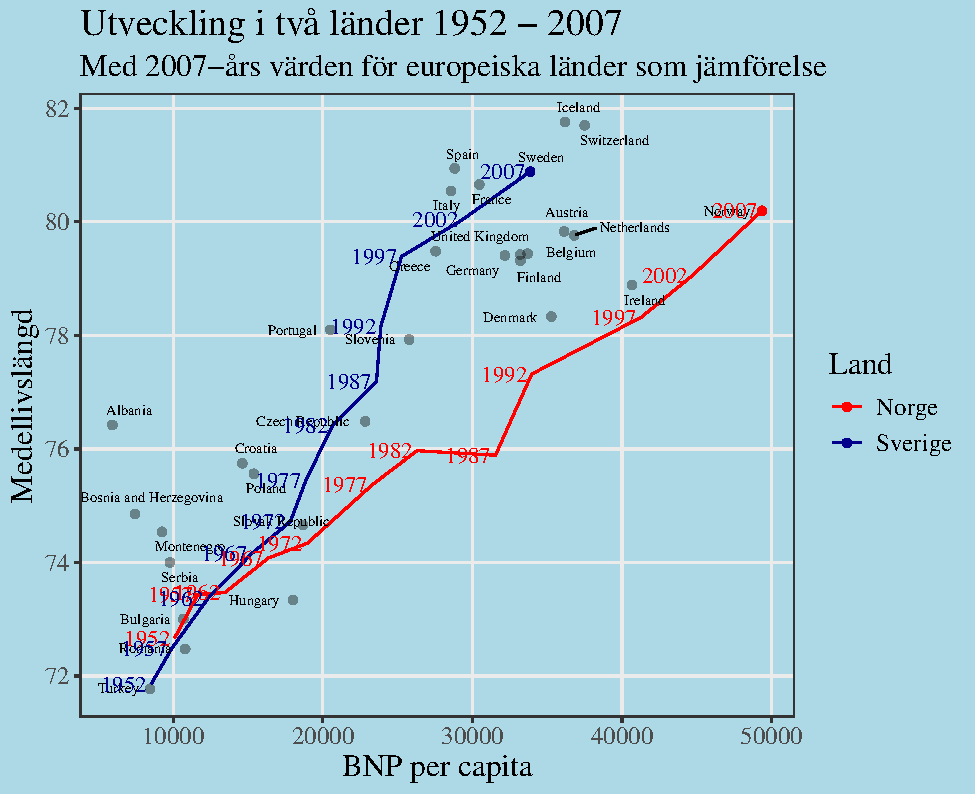
\includegraphics{R-anvisningar_files/figure-latex/unnamed-chunk-54-1} \end{center}

\begin{exercise}[Dekonstruera grafen]
Vilka geografiska former (punkter, linjer ytor) visas i grafen och hur är de kopplade till datans variabler? Vilka ändringar har gjorts från standardtemat (bakgrundsfärg, typsnitt, teckenstorlek)?
\end{exercise}

\begin{exercise}[Rekonstrera grafen]
Använd en chatbot (såsom Microsofts co-pilot eller OpenAIs ChatGPT) för att rekonstrera grafen. Börja med att beskriva grafen i ord och be om R-kod. Klipp ut koden och kör i R. Läs koden du fått. Finns det några delar som är svåra att förstå. Med vissa chatverktyg kan man också klippa in bilden och be om den bakomliggande koden.
\end{exercise}

\begin{exercise}[Steg i Excel]
Hur skulle man gå tillväga för att skapa samma graf i Excel? Be en chatbot om en stegvis instruktion.
\end{exercise}

\chapter{Beskrivande statistik}\label{beskrivande-statistik}

Datorövning 2 handlar om beräkning av beskrivande statistik i R. Efter övningen ska vi kunna

\begin{itemize}
\tightlist
\item
  Importera data från en excelfil,
\item
  Beräkna lämpliga lägesmått för en variabel,
\item
  Beräkna lämpliga spridningsmått för en variabel,
\item
  Konstruera grafer som jämför två eller flera gruppers läge och spridning.
\end{itemize}

\section{Repetition från datorövning 1}\label{repetition-fruxe5n-datoruxf6vning-1}

När man arbetar i R är det klokt att använda ett avancerat gränssnitt som RStudio och att skriva sin kod i ett separat skript. I RStudio kan man starta ett nytt skript genom \emph{Ctrl + Shift + N}.

Mycket funktionalitet i R ligger i tilläggspaket (\emph{Packages}). Paket måste installeras första gången de används och laddas varje session de används, t.ex.

\begin{Shaded}
\begin{Highlighting}[]
\CommentTok{\# install.packages("tidyverse") \# Installera tidyverse}
\FunctionTok{library}\NormalTok{(tidyverse)              }\CommentTok{\# Ladda ett paket}
\end{Highlighting}
\end{Shaded}

Objekt skapas med \emph{assign}-pilen \texttt{\textless{}-}. Det är ett sätt att importera data till R. Det är dock vanligare importera från en extern fil. Mer om det senare.

Vi arbetar nästan alltid med data på tabellformat där variablerna är kolumner och observationerna rader. I gapminder-datan ges raderna av ett land för ett visst år.

\begin{Shaded}
\begin{Highlighting}[]
\FunctionTok{library}\NormalTok{(gapminder)}
\NormalTok{gapminder                       }\CommentTok{\# Skriv ut objektet gapminder}
\end{Highlighting}
\end{Shaded}

Funktioner agerar på objekt och ger något utfall. Här nedan beräknas medelvärdet av livslängd med funktionen \texttt{mean()}. Dollartecknet används för att ange en specifik kolumn i dataobjektet. Funktioner styrs av möjliga argument - här används \texttt{na.rm} för att ange att saknade värden inte ska tas med i beräkningen

\begin{Shaded}
\begin{Highlighting}[]
\FunctionTok{mean}\NormalTok{(gapminder}\SpecialCharTok{$}\NormalTok{lifeExp, }\AttributeTok{na.rm =}\NormalTok{ T) }\CommentTok{\# Beräkna medel av lifeExp}
\end{Highlighting}
\end{Shaded}

\begin{verbatim}
## [1] 59.47444
\end{verbatim}

Funktionerna \texttt{filter()} och \texttt{select()} kan användas för att välja kolumner och rader. Funktioner kan länkas samman med en pipe \texttt{\%\textgreater{}\%} för att skapa sekvenser av funktioner. Man kan tänka på pipen som \emph{och sen}.

\begin{Shaded}
\begin{Highlighting}[]
\NormalTok{gapminder }\SpecialCharTok{\%\textgreater{}\%}
  \FunctionTok{filter}\NormalTok{(country }\SpecialCharTok{==} \StringTok{"Norway"}\NormalTok{, year }\SpecialCharTok{\textgreater{}} \DecValTok{1972}\NormalTok{) }\SpecialCharTok{\%\textgreater{}\%}
  \FunctionTok{select}\NormalTok{(country, lifeExp)}
\end{Highlighting}
\end{Shaded}

Slutligen tittade vi på grafer med ggplot2-paketet. En ggplot byggs upp med tre grundelar: data, geometrier (grafens objekt och former), och \emph{aesthetics} (utseende och placering av geometrierna). I ett enkelt spridningsdiagram är data två numeriska variabler, geometrierna är punkter, och punkternas placering ges av en x-koordinat och en y-koordinat. Ytterligare \emph{aesthetics} kan vara punkternas färger (\texttt{color}) och storlek (\texttt{size}).

\begin{Shaded}
\begin{Highlighting}[]
\NormalTok{dat\_small }\OtherTok{\textless{}{-}}\NormalTok{ gapminder }\SpecialCharTok{\%\textgreater{}\%} \FunctionTok{filter}\NormalTok{(year }\SpecialCharTok{==} \DecValTok{2007}\NormalTok{)}
\FunctionTok{ggplot}\NormalTok{(dat\_small, }\FunctionTok{aes}\NormalTok{(}\AttributeTok{x =}\NormalTok{ gdpPercap, }\AttributeTok{y =}\NormalTok{ lifeExp, }
                      \AttributeTok{size =}\NormalTok{ pop, }\AttributeTok{color =}\NormalTok{ continent)) }\SpecialCharTok{+}
  \FunctionTok{geom\_point}\NormalTok{()}
\end{Highlighting}
\end{Shaded}

\section{Import av data från en Excelfil}\label{import-av-data-fruxe5n-en-excelfil}

Inom vetenskapen är Excel det vanligaste filformatet för mindre datamängder. Till den här delen ska vi återigen arbeta med data från \emph{Gapminder}.

\begin{exercise}[Excelfil från Canvas]
Hitta excelfilen \emph{Gapminder.xlsx} på Canvas och ladda ner den. Hitta mappen som filen laddats ned till.
\end{exercise}

I R kan man läsa in data från en Excel-fil med funktionen \texttt{read\_excel()} från paketet \texttt{readxl}. Som argument till funktionen sätts filens sökväg - dess placering på hårddisken. Stycket nedan importerar från en excelfil som ligger på hårddisken \emph{C:} i mappen \emph{Downloads}, under \emph{User\_name}, under \emph{Users}.

\begin{Shaded}
\begin{Highlighting}[]
\FunctionTok{library}\NormalTok{(readxl)  }\CommentTok{\# Ladda readxl}
\end{Highlighting}
\end{Shaded}

\begin{Shaded}
\begin{Highlighting}[]
\NormalTok{gapminder }\OtherTok{\textless{}{-}} \FunctionTok{read\_excel}\NormalTok{(}\StringTok{"C:/Users/Name/Downloads/Gapminder.xlsx"}\NormalTok{)}
\CommentTok{\# Läs in från en lokal excelfil}
\NormalTok{gapminder}
\end{Highlighting}
\end{Shaded}

\begin{exercise}[Importera från excelfil]
Var ligger den nedladdade filen \emph{Gapminder.xlsx}? Gör lämplig ändring i koden ovan för att läsa in data från den filen. Notera att R använder högerlutande snedstreck \texttt{/}, så om en kopierad sökväg har vänster-snedstreck måste de ändras. Kontrollera att datan blivit korrekt inläst genom att köra objektnamnet \texttt{gapminder}.
\end{exercise}

En R-session har alltid en grundmapp, ett \emph{Working directory}. Man kan se vilken mapp det är genom att köra

\begin{Shaded}
\begin{Highlighting}[]
\FunctionTok{getwd}\NormalTok{() }\CommentTok{\# Ange working directory}
\end{Highlighting}
\end{Shaded}

En filsökväg kan anges antingen som en fullständig sökväg, som ovan, eller relativt \emph{working directory}. Om man till exempel har en fil \emph{Gapminder.xlsx} som ligger i en mapp \emph{Data} som i sin tur ligger i \emph{working directory}, kan man importera data från filen med

\begin{Shaded}
\begin{Highlighting}[]
\NormalTok{gapminder }\OtherTok{\textless{}{-}} \FunctionTok{read\_excel}\NormalTok{(}\StringTok{"Data/Gapminder.xlsx"}\NormalTok{)}
\CommentTok{\# Läs in från en lokal excelfil (relativt wd)}
\NormalTok{gapminder }
\end{Highlighting}
\end{Shaded}

\begin{exercise}[Working directory]
Identifiera \emph{working directory} för din nuvarande Rs-session genom att köra \texttt{getwd()}.
\end{exercise}

RStudio har också en inbyggd funktionalitet för att importera data. Man kan hitta den genom att gå till \emph{Environment}-fliken och sedan \emph{Import Dataset}. Det kan vara en bra hjälp, i synnerhet om man vill sätta datatyp för någon specifik kolumn.

Om du inte har tillgång till Canvas kan Gapminder-datan alternativt hämtas från paketet Gapminder.

\begin{Shaded}
\begin{Highlighting}[]
\CommentTok{\# install.packages("gapminder")}
\FunctionTok{library}\NormalTok{(gapminder)             }
\NormalTok{gapminder                      }
\end{Highlighting}
\end{Shaded}

\section{\texorpdfstring{Ändra och skapa nya kolumner med \texttt{mutate}}{Ändra och skapa nya kolumner med mutate}}\label{uxe4ndra-och-skapa-nya-kolumner-med-mutate}

Variabler kan omräknas och nya variabler kan skapas med \texttt{mutate}-funktionen. I gapminder-datan finns bnp per capita. Om man vill ha nationell BNP kan man skapa en ny kolumn och beräkna den som bnp per capita gånger populationen.

\begin{Shaded}
\begin{Highlighting}[]
\NormalTok{gapminder }\OtherTok{\textless{}{-}}\NormalTok{ gapminder }\SpecialCharTok{\%\textgreater{}\%}             \CommentTok{\# Ta datan, och sen}
  \FunctionTok{mutate}\NormalTok{(}\AttributeTok{gdp =}\NormalTok{ gdpPercap }\SpecialCharTok{*}\NormalTok{ pop)        }\CommentTok{\# Beräkna bnp}
\end{Highlighting}
\end{Shaded}

Den inledande delen med \texttt{gapminder\ \textless{}-} gör så att utfallet av beräkningen sparas i objektet \texttt{gapminder}.
Vi kan skriva ut objektet och se resultatet av beräkningen:

\begin{Shaded}
\begin{Highlighting}[]
\NormalTok{gapminder}
\end{Highlighting}
\end{Shaded}

Om man vill skapa en kolumn med mellanrum i namnet måste man skriva namnet inom \emph{backticks} ` för att ange att namnet ska tolkas som en enhet. Jag rekommenderar att undvika mellanrum i kolumnnamn och istället använda stora bokstäver eller understreck för ett nytt ord (\texttt{NationalGDP} eller \texttt{National\_GDP}).

\begin{Shaded}
\begin{Highlighting}[]
\NormalTok{gapminder }\OtherTok{\textless{}{-}}\NormalTok{ gapminder }\SpecialCharTok{\%\textgreater{}\%} 
  \FunctionTok{mutate}\NormalTok{(}\StringTok{\textasciigrave{}}\AttributeTok{National GDP}\StringTok{\textasciigrave{}} \OtherTok{=}\NormalTok{ gdpPercap }\SpecialCharTok{*}\NormalTok{ pop)}
\NormalTok{gapminder}
\end{Highlighting}
\end{Shaded}

\section{Sammanfattande lägesmått}\label{sammanfattande-luxe4gesmuxe5tt}

Den importerade datan anger medellivslängd, populationsstorlek och bnp per capita per land och år. Vi kan börja med att producera en bubbelgraf över datan - en av de presentationer Gapminder ofta använder. En bubbelgraf är ett spridningsdiagram där punktens storlek beror på en tredje variabel.

\begin{Shaded}
\begin{Highlighting}[]
\FunctionTok{ggplot}\NormalTok{(gapminder, }\FunctionTok{aes}\NormalTok{(}\AttributeTok{x =}\NormalTok{ gdpPercap, }\AttributeTok{y =}\NormalTok{ lifeExp, }
                      \AttributeTok{size =}\NormalTok{ pop, }\AttributeTok{color =}\NormalTok{ continent)) }\SpecialCharTok{+}
  \FunctionTok{geom\_point}\NormalTok{() }\SpecialCharTok{+}
  \FunctionTok{facet\_wrap}\NormalTok{(}\SpecialCharTok{\textasciitilde{}}\NormalTok{ year)}
\end{Highlighting}
\end{Shaded}

En interaktiv version kan vara bra om man vill identifiera någon specifik punkt.

\begin{Shaded}
\begin{Highlighting}[]
\NormalTok{g }\OtherTok{\textless{}{-}} \FunctionTok{ggplot}\NormalTok{(gapminder, }\FunctionTok{aes}\NormalTok{(}\AttributeTok{x =}\NormalTok{ gdpPercap, }\AttributeTok{y =}\NormalTok{ lifeExp, }\AttributeTok{size =}\NormalTok{ pop, }
                           \AttributeTok{color =}\NormalTok{ continent, }\AttributeTok{text =}\NormalTok{ country)) }\SpecialCharTok{+}
  \FunctionTok{geom\_point}\NormalTok{() }\SpecialCharTok{+}
  \FunctionTok{facet\_wrap}\NormalTok{(}\SpecialCharTok{\textasciitilde{}}\NormalTok{ year)}

\CommentTok{\# install.packages("plotly")  \# Kör om ej installerat tidigare}
\FunctionTok{library}\NormalTok{(plotly)               }\CommentTok{\# Ladda paketet plotly}
\FunctionTok{ggplotly}\NormalTok{(g)                   }\CommentTok{\# Interaktiv graf g}
\end{Highlighting}
\end{Shaded}

Under föreläsningen såg vi exempel på två lägesmått: medelvärdet (egentligen det \emph{aritmetiska} medelvärdet) och medianen. De har bägge enkla funktioner i R: \texttt{mean()} respektive \texttt{median()}. Vi plockar ut en variabel ur datan och beräknar bägge.

\begin{Shaded}
\begin{Highlighting}[]
\NormalTok{gapminder}\SpecialCharTok{$}\NormalTok{gdpPercap         }\CommentTok{\# Vektorn med data}
\FunctionTok{mean}\NormalTok{(gapminder}\SpecialCharTok{$}\NormalTok{gdpPercap)   }\CommentTok{\# Beräkna medelvärdet}
\FunctionTok{median}\NormalTok{(gapminder}\SpecialCharTok{$}\NormalTok{gdpPercap) }\CommentTok{\# Beräkna medianen}
\end{Highlighting}
\end{Shaded}

Samma sak kan göras med en pipe \texttt{\%\textgreater{}\%} och \texttt{summarise()}.

\begin{Shaded}
\begin{Highlighting}[]
\NormalTok{gapminder }\SpecialCharTok{\%\textgreater{}\%}
  \FunctionTok{summarise}\NormalTok{(}\AttributeTok{Mean =} \FunctionTok{mean}\NormalTok{(gdpPercap),}
            \AttributeTok{Median =} \FunctionTok{median}\NormalTok{(gdpPercap))}
\end{Highlighting}
\end{Shaded}

\begin{exercise}[Lägesmått av livslängd]
Gör lämpliga ändringar i exemplet ovan för att beräkna lägesmått för medellivslängd (\texttt{lifeExp}).
\end{exercise}

Den andra lösningen, med en pipe och \texttt{summarise()}, kan enkelt utvecklas med ett \texttt{group\_by()}-steg för att beräkna medel och median per någon grupp, t.ex. per år.

\begin{Shaded}
\begin{Highlighting}[]
\NormalTok{gapminder }\SpecialCharTok{\%\textgreater{}\%}                           \CommentTok{\# Ta datan, och sen}
  \FunctionTok{group\_by}\NormalTok{(year) }\SpecialCharTok{\%\textgreater{}\%}                    \CommentTok{\# gruppera efter år, och}
  \FunctionTok{summarise}\NormalTok{(}\AttributeTok{Mean =} \FunctionTok{mean}\NormalTok{(gdpPercap),     }\CommentTok{\# beräkna medelvärde och}
            \AttributeTok{Median =} \FunctionTok{median}\NormalTok{(gdpPercap)) }\CommentTok{\# medianen av gdpPercap}
\end{Highlighting}
\end{Shaded}

\begin{exercise}[Lägesmått per kontinent]
Gör lämpliga ändringar i exemplet ovan för att beräkna lägesmått per kontinent. Vad måste läggas till för att också beräkna maximum och minimum per kontinent (funktionerna \texttt{max()} och \texttt{min()})?
\end{exercise}

\begin{exercise}[Upprepade mätningar]
Finns det några problem med att beräkna medelvärde per kontinent på den här datan?
\end{exercise}

I vetenskapliga publikationer redovisas medelvärden ofta med ett stapeldiagram. Som exempel ges staplar för medelvärdet av bnp per kontinent för 2007.

\begin{Shaded}
\begin{Highlighting}[]
\NormalTok{dat\_gdp\_2007 }\OtherTok{\textless{}{-}}\NormalTok{ gapminder }\SpecialCharTok{\%\textgreater{}\%}       \CommentTok{\# Ta datan, och sen}
  \FunctionTok{filter}\NormalTok{(year }\SpecialCharTok{==} \DecValTok{2007}\NormalTok{) }\SpecialCharTok{\%\textgreater{}\%}          \CommentTok{\# filtrera för 2007, och sen}
  \FunctionTok{group\_by}\NormalTok{(continent) }\SpecialCharTok{\%\textgreater{}\%}           \CommentTok{\# gruppera kontinenter, och}
  \FunctionTok{summarise}\NormalTok{(}\AttributeTok{Mean =} \FunctionTok{mean}\NormalTok{(gdpPercap)) }\CommentTok{\# beräkna medelvärdet}

\FunctionTok{ggplot}\NormalTok{(dat\_gdp\_2007, }\FunctionTok{aes}\NormalTok{(continent, Mean)) }\SpecialCharTok{+}
  \FunctionTok{geom\_col}\NormalTok{()                  }\CommentTok{\# Illustrera med kolumner (columns)}
\end{Highlighting}
\end{Shaded}

\begin{exercise}[Graf för livslängd]
Gör om stapeldiagrammet. Denna gång med livslängd (\texttt{lifeExp}) istället för bnp per capita (\texttt{gdpPercap}).
\end{exercise}

\section{Sammanfattande spridningsmått}\label{sammanfattande-spridningsmuxe5tt}

Under föreläsningarna såg vi några mått på spridning: varians, standardavvikelse och kvartilavstånd (IQR, \emph{inter-quartile range}). De har alla motsvarande funktioner i R (\texttt{var()}, \texttt{sd()}, och \texttt{IQR()}) som kan användas på samma sätt som funktionerna för lägesmått.

\begin{Shaded}
\begin{Highlighting}[]
\NormalTok{gapminder}\SpecialCharTok{$}\NormalTok{gdpPercap      }\CommentTok{\# Vektorn med data}

\FunctionTok{var}\NormalTok{(gapminder}\SpecialCharTok{$}\NormalTok{gdpPercap) }\CommentTok{\# Beräkna varians}
\FunctionTok{sd}\NormalTok{(gapminder}\SpecialCharTok{$}\NormalTok{gdpPercap)  }\CommentTok{\# Beräkna standardavvikelse}
\FunctionTok{IQR}\NormalTok{(gapminder}\SpecialCharTok{$}\NormalTok{gdpPercap) }\CommentTok{\# Beräkna kvartilavstånd}
\end{Highlighting}
\end{Shaded}

Alternativt med en pipe och \texttt{summarise()}.

\begin{Shaded}
\begin{Highlighting}[]
\NormalTok{gapminder }\SpecialCharTok{\%\textgreater{}\%}                       \CommentTok{\# Ta datan, och}
  \FunctionTok{summarise}\NormalTok{(}\AttributeTok{Var =} \FunctionTok{var}\NormalTok{(gdpPercap),   }\CommentTok{\# beräkna varians,}
            \AttributeTok{Sd =} \FunctionTok{sd}\NormalTok{(gdpPercap),     }\CommentTok{\# standardavvikelse,}
            \AttributeTok{IQR =} \FunctionTok{IQR}\NormalTok{(gdpPercap))   }\CommentTok{\# och kvartilavstånd}
\end{Highlighting}
\end{Shaded}

Lösningen med pipe och \texttt{summarise()} kan som tidigare utvecklas med \texttt{group\_by()}.

\begin{Shaded}
\begin{Highlighting}[]
\NormalTok{gapminder }\SpecialCharTok{\%\textgreater{}\%}
  \FunctionTok{group\_by}\NormalTok{(year) }\SpecialCharTok{\%\textgreater{}\%}
  \FunctionTok{summarise}\NormalTok{(}\AttributeTok{Varians =} \FunctionTok{var}\NormalTok{(gdpPercap),}
            \AttributeTok{Standardavvikelse =} \FunctionTok{sd}\NormalTok{(gdpPercap),}
\NormalTok{            Kvartilavstånd }\OtherTok{=} \FunctionTok{IQR}\NormalTok{(gdpPercap))}
\end{Highlighting}
\end{Shaded}

\begin{exercise}[Graf för livslängd]
Gör lämpliga ändringar i det sista exempel för att istället beräkna spridningsmått för livslängd.
\end{exercise}

Vi avslutar med tre vanliga illustrationer av vetenskaplig data - ett linjediagram med felstaplar, ett stapeldiagram med felstaplar, och ett lådagram. För linjediagrammet beräknar vi medelvärdet och spridningsmått för bnp över år och kontinent. Som spridningsmått använder vi standard error (sv. \emph{medelfel}), vilket beräknas som standardavvikelse delat på roten ur antalet observationer. Funktionen \texttt{n()} ger antalet observationer per kontinent och år.

\begin{Shaded}
\begin{Highlighting}[]
\NormalTok{dat\_year\_continent }\OtherTok{\textless{}{-}}\NormalTok{ gapminder }\SpecialCharTok{\%\textgreater{}\%}
  \FunctionTok{group\_by}\NormalTok{(year, continent) }\SpecialCharTok{\%\textgreater{}\%}
  \FunctionTok{summarise}\NormalTok{(}\AttributeTok{Mean =} \FunctionTok{mean}\NormalTok{(gdpPercap),}
            \AttributeTok{SE =} \FunctionTok{sd}\NormalTok{(gdpPercap) }\SpecialCharTok{/} \FunctionTok{sqrt}\NormalTok{(}\FunctionTok{n}\NormalTok{()))}
\NormalTok{dat\_year\_continent}
\end{Highlighting}
\end{Shaded}

Med \texttt{ggplot2} kan vi bygga ett linjediagram med \texttt{geom\_line()} och lägga till felstaplar med \texttt{geom\_errorbar()}. Den senare behöver \texttt{aes()}-argument för \texttt{ymin} och \texttt{ymax} - nedre och övre del av felstapeln. Vi sätter dem till medelvärdet minus respektive plus ett medelfel.

\begin{Shaded}
\begin{Highlighting}[]
\FunctionTok{ggplot}\NormalTok{(dat\_year\_continent, }\FunctionTok{aes}\NormalTok{(}\AttributeTok{x =}\NormalTok{ year, }\AttributeTok{y =}\NormalTok{ Mean, }
                               \AttributeTok{color =}\NormalTok{ continent)) }\SpecialCharTok{+}
  \FunctionTok{geom\_line}\NormalTok{() }\SpecialCharTok{+}
  \FunctionTok{geom\_errorbar}\NormalTok{(}\FunctionTok{aes}\NormalTok{(}\AttributeTok{ymin =}\NormalTok{ Mean }\SpecialCharTok{{-}}\NormalTok{ SE, }\AttributeTok{ymax =}\NormalTok{ Mean }\SpecialCharTok{+}\NormalTok{ SE))}
\end{Highlighting}
\end{Shaded}

\begin{exercise}[Bredd]
Felstaplarna från \texttt{geom\_errorbar()} har väldigt breda ändar. Använd hjälpsidan för geomet \texttt{?geom\_errorbar}, i synnerhet exemplen längst ned, och se om det går att ändra bredden.
\end{exercise}

En graf med staplar och felstaplar kan konstrueras på ett liknande sätt. Följande exempel visar staplar över livslängd per kontinent. Felstapeln ges av standardavvikelsen.

\begin{Shaded}
\begin{Highlighting}[]
\NormalTok{dat\_2007 }\OtherTok{\textless{}{-}}\NormalTok{ gapminder }\SpecialCharTok{\%\textgreater{}\%}          \CommentTok{\# Ta datan, och sen}
  \FunctionTok{filter}\NormalTok{(year }\SpecialCharTok{==} \DecValTok{2007}\NormalTok{) }\SpecialCharTok{\%\textgreater{}\%}        \CommentTok{\# filtrera på år, och sen}
  \FunctionTok{group\_by}\NormalTok{(continent) }\SpecialCharTok{\%\textgreater{}\%}         \CommentTok{\# gruppera efter kontinent,}
  \FunctionTok{summarise}\NormalTok{(}\AttributeTok{Mean =} \FunctionTok{mean}\NormalTok{(lifeExp), }\CommentTok{\# summera med medelvärde,}
            \AttributeTok{SD =} \FunctionTok{sd}\NormalTok{(lifeExp))     }\CommentTok{\# och standardavvikelse}
\NormalTok{dat\_2007}
\end{Highlighting}
\end{Shaded}

Vi bygger en ggplot med \texttt{geom\_col()} och \texttt{geom\_errorbar()}. Felstapels konstruktion kan anges i en notis med funktionen \texttt{labs()}.

\begin{Shaded}
\begin{Highlighting}[]
\FunctionTok{ggplot}\NormalTok{(dat\_2007, }\FunctionTok{aes}\NormalTok{(continent, Mean, }\AttributeTok{fill =}\NormalTok{ continent)) }\SpecialCharTok{+}
  \FunctionTok{geom\_col}\NormalTok{()}\SpecialCharTok{+}                                            
  \FunctionTok{geom\_errorbar}\NormalTok{(}\FunctionTok{aes}\NormalTok{(}\AttributeTok{ymin =}\NormalTok{ Mean }\SpecialCharTok{{-}}\NormalTok{ SD, }\AttributeTok{ymax =}\NormalTok{ Mean }\SpecialCharTok{+}\NormalTok{ SD)) }\SpecialCharTok{+}
  \FunctionTok{labs}\NormalTok{(}\AttributeTok{title =} \StringTok{"Average life expectancy by continent, 2007"}\NormalTok{,}
       \AttributeTok{caption =} \StringTok{"Errorbars given by mean +/{-} standard deviation.}
\StringTok{       Source: Gapminder"}\NormalTok{)}
\end{Highlighting}
\end{Shaded}

\begin{exercise}[Staplar för 1982]
Gör lämpliga ändringar i exempel ovan för att konstruera ett stapeldiagram med felstaplar för året 1982 och variabeln medellivslängd.
\end{exercise}

Ett lådagram anger fördelningen av en variabel genom att illustrera minimum, maximum och kvartiler. Kvartiler är mått som delar en datamängd i fyra lika stora delar (så att en fjärdedel ligger under första kvartilen, en fjärdedel mellan första och andra kvartil, och så vidare). Med \texttt{ggplot2} kan vi bygga ett lådagram med \texttt{geom\_boxplot()}. Exempel ger en låda per år och kontinent.

\begin{Shaded}
\begin{Highlighting}[]
\FunctionTok{ggplot}\NormalTok{(gapminder, }\FunctionTok{aes}\NormalTok{(year, lifeExp, }\AttributeTok{fill =}\NormalTok{ continent, }
                      \AttributeTok{group =}\NormalTok{ year)) }\SpecialCharTok{+}
  \FunctionTok{geom\_boxplot}\NormalTok{() }\SpecialCharTok{+}                                                     
  \FunctionTok{facet\_wrap}\NormalTok{(}\SpecialCharTok{\textasciitilde{}}\NormalTok{ continent)                                              }
\end{Highlighting}
\end{Shaded}

\begin{exercise}[Group-argumentet]
I lådagrammet används argumentet \texttt{group}. Vad gör det? Vad händer om man tar bort det?
\end{exercise}

\section{Ordna upp beskrivande statistik och exportera}\label{ordna-upp-beskrivande-statistik-och-exportera}

Efter att ha beräknat någon beskrivande statistik kan det vara bra att titta på hur resultaten kan snyggas upp och exporteras i något lämpligt format. Ta den tabell med medelvärden vi producerade i ett tidigare exempel.

\begin{Shaded}
\begin{Highlighting}[]
\NormalTok{dat\_2007 }\OtherTok{\textless{}{-}}\NormalTok{ gapminder }\SpecialCharTok{\%\textgreater{}\%}         \CommentTok{\# Ta datan, och sen}
  \FunctionTok{filter}\NormalTok{(year }\SpecialCharTok{==} \DecValTok{2007}\NormalTok{) }\SpecialCharTok{\%\textgreater{}\%}        \CommentTok{\# filtrera på år, och sen}
  \FunctionTok{group\_by}\NormalTok{(continent) }\SpecialCharTok{\%\textgreater{}\%}         \CommentTok{\# gruppera efter kontinent,}
  \FunctionTok{summarise}\NormalTok{(}\AttributeTok{Mean =} \FunctionTok{mean}\NormalTok{(lifeExp), }\CommentTok{\# summera med medelvärde,}
            \AttributeTok{SD =} \FunctionTok{sd}\NormalTok{(lifeExp))     }\CommentTok{\# och standardavvikelse}
\NormalTok{dat\_2007}
\end{Highlighting}
\end{Shaded}

Objekt kan exporteras från R på liknande som det importeras - med särskilda exportfunktioner (\emph{write}-funktioner) beroende på filtyp. För att exportera till en csv-fil man man använda \texttt{write\_csv()}. Ingående argument är det objekt man vill exportera och den fil man vill exportera till. R ger ingen varning om man skriver över en existerande fil, så var lite försiktiga här.

Precis som vid import använder R \emph{working directory} om inget annat anges. Följande exporterar objektet \texttt{dat\_2007} till en csv-fil \emph{Exporterad data från R.csv} i \emph{working directory}.

\begin{Shaded}
\begin{Highlighting}[]
\FunctionTok{getwd}\NormalTok{()                          }\CommentTok{\# Se nuvarande working directory}
\FunctionTok{write\_csv}\NormalTok{(dat\_2007, }\StringTok{"Exporterad data från R.csv"}\NormalTok{) }\CommentTok{\# Exportera data}
\end{Highlighting}
\end{Shaded}

Därifrån skulle man kunna öppna filen i något kalkylprogram, snygga till layouten, och sedan klippa in i ett textdokument.

\section{Kumulativt medelvärde}\label{kumulativt-medelvuxe4rde}

Om man har data som av någon anledning samlas in i sekvens kan det vara intressant att beräkna och illustrera den med ett \emph{kumulativt medelvärde}. En serie med kumulativa medelvärden beräknas genom att för varje nytt värde ta medelvärden av de värden man hittills samlat in - vid tio värden tar man medelvärdet av de tio, vid elva värden medelvärdet av de elva, och så vidare.

Med de tärningsvärden vi hade innan kan vi beräkna ett kumulativt medelvärde genom att först beräkna summan med \texttt{cumsum()} och sedan dela på antalet kast. För att förenkla beräkningen av antalen tar vi fram sekvensen med antal kast i ett \texttt{mutate()}-steg.

\begin{Shaded}
\begin{Highlighting}[]
\NormalTok{dat\_dice }\OtherTok{\textless{}{-}} \FunctionTok{data.frame}\NormalTok{(}\AttributeTok{Utfall =} \FunctionTok{c}\NormalTok{(}\DecValTok{6}\NormalTok{,}\DecValTok{3}\NormalTok{,}\DecValTok{2}\NormalTok{,}\DecValTok{3}\NormalTok{,}\DecValTok{5}\NormalTok{)) }\SpecialCharTok{\%\textgreater{}\%}
  \FunctionTok{mutate}\NormalTok{(}\AttributeTok{Kast =} \DecValTok{1}\SpecialCharTok{:}\FunctionTok{n}\NormalTok{())                           }
\NormalTok{dat\_dice}

\NormalTok{dat\_dice }\OtherTok{\textless{}{-}}\NormalTok{ dat\_dice }\SpecialCharTok{\%\textgreater{}\%}
  \FunctionTok{mutate}\NormalTok{(}\AttributeTok{kumulativ\_summa =} \FunctionTok{cumsum}\NormalTok{(Utfall),  }
\NormalTok{         kumulativt\_medelvärde }\OtherTok{=}\NormalTok{ kumulativ\_summa }\SpecialCharTok{/}\NormalTok{ Kast)}
\NormalTok{dat\_dice}
\end{Highlighting}
\end{Shaded}

\begin{exercise}[Kumulativt medelvärde]

Vad ska läggas till för att stycket nedan ska ge en linjegraf över medelvärdet?

\begin{Shaded}
\begin{Highlighting}[]
\FunctionTok{ggplot}\NormalTok{(dat\_dice, }\FunctionTok{aes}\NormalTok{(}\AttributeTok{x =}\NormalTok{ Kast, }\AttributeTok{y =}\NormalTok{ \_\_\_)) }\SpecialCharTok{+}
  \FunctionTok{\_\_\_}\NormalTok{()}
\end{Highlighting}
\end{Shaded}

\end{exercise}

\begin{exercise}[Fler tärningskast]

Kasta din tärning ytterligare några gånger, gärna på en mjuk yta. Fyll i dina utfall och gör grafen från föregående uppgift. Kan man se en tendens för medelvärdet att minska i varians vid fler kast? Svänger kurvan in mot något specifikt värde?

\begin{Shaded}
\begin{Highlighting}[]
\NormalTok{dat\_dice }\OtherTok{\textless{}{-}} \FunctionTok{data.frame}\NormalTok{(}\AttributeTok{Utfall =} \FunctionTok{c}\NormalTok{(\_\_\_)) }\SpecialCharTok{\%\textgreater{}\%} 
  \FunctionTok{mutate}\NormalTok{(}\AttributeTok{Kast =} \DecValTok{1}\SpecialCharTok{:}\FunctionTok{n}\NormalTok{(),                                 }
         \AttributeTok{kumulativ\_summa =} \FunctionTok{cumsum}\NormalTok{(Utfall),           }
\NormalTok{         kumulativt\_medelvärde }\OtherTok{=}\NormalTok{ kumulativ\_summa }\SpecialCharTok{/}\NormalTok{ Kast)}
\NormalTok{dat\_dice}
\end{Highlighting}
\end{Shaded}

\end{exercise}

\begin{exercise}[Kumulativ frekvens]

Om man vill titta på andelen gånger ett visst utfall inträffat talar man om \emph{kumulativ frekvens} snarare än \emph{kumulativt medelvärde}. Använd stycket nedan för att titta på andelen gånger utfallet varit en etta (ett \emph{positivt} utfall, i begreppets kliniska mening). Om ett inte är ett möjligt utfall på din tärning, ändra ettan till något mer lämpligt.

\begin{Shaded}
\begin{Highlighting}[]
\NormalTok{dat\_dice }\OtherTok{\textless{}{-}} \FunctionTok{data.frame}\NormalTok{(}\AttributeTok{Utfall =} \FunctionTok{c}\NormalTok{(\_\_\_)) }\SpecialCharTok{\%\textgreater{}\%} 
  \FunctionTok{mutate}\NormalTok{(}\AttributeTok{Kast =} \DecValTok{1}\SpecialCharTok{:}\FunctionTok{n}\NormalTok{(),}
         \AttributeTok{positivt\_utfall =}\NormalTok{ Utfall }\SpecialCharTok{==} \DecValTok{1}\NormalTok{,              }
         \AttributeTok{kumulativt\_antal =} \FunctionTok{cumsum}\NormalTok{(positivt\_utfall),}
         \AttributeTok{kumulativ\_frekvens =}\NormalTok{ kumulativt\_antal }\SpecialCharTok{/}\NormalTok{ Kast)}
\NormalTok{dat\_dice}

\FunctionTok{ggplot}\NormalTok{(dat\_dice, }\FunctionTok{aes}\NormalTok{(}\AttributeTok{x =}\NormalTok{ Kast, }\AttributeTok{y =}\NormalTok{ kumulativ\_frekvens)) }\SpecialCharTok{+}
  \FunctionTok{geom\_line}\NormalTok{()}
\end{Highlighting}
\end{Shaded}

\end{exercise}

\section{\texorpdfstring{Tredimensionella grafer med \texttt{plotly}}{Tredimensionella grafer med plotly}}\label{tredimensionella-grafer-med-plotly}

De två avslutande avsnitten är mindre viktiga och kan läsas i mån av tid.

Paketet \texttt{plotly} kan användas för att göra interaktiva graf och grafer med tre dimensioner. Börja med att ladda paketet.

\begin{Shaded}
\begin{Highlighting}[]
\FunctionTok{library}\NormalTok{(plotly)}
\end{Highlighting}
\end{Shaded}

Vi börjar med ett enkelt exempel på en 3d-graf med lite skapad data.

\begin{Shaded}
\begin{Highlighting}[]
\NormalTok{dat\_ex }\OtherTok{\textless{}{-}} \FunctionTok{data.frame}\NormalTok{(}\AttributeTok{Var1 =} \FunctionTok{c}\NormalTok{(}\DecValTok{1}\NormalTok{,}\DecValTok{2}\NormalTok{,}\DecValTok{3}\NormalTok{), }\AttributeTok{Var2 =} \FunctionTok{c}\NormalTok{(}\DecValTok{3}\NormalTok{,}\DecValTok{1}\NormalTok{,}\DecValTok{2}\NormalTok{), }
                     \AttributeTok{Var3 =} \FunctionTok{c}\NormalTok{(}\DecValTok{2}\NormalTok{,}\DecValTok{3}\NormalTok{,}\DecValTok{1}\NormalTok{), }\AttributeTok{Type =} \FunctionTok{c}\NormalTok{(}\StringTok{"A"}\NormalTok{, }\StringTok{"B"}\NormalTok{, }\StringTok{"C"}\NormalTok{))}
\NormalTok{dat\_ex}

\FunctionTok{plot\_ly}\NormalTok{(dat\_ex, }\AttributeTok{x =} \SpecialCharTok{\textasciitilde{}}\NormalTok{Var1, }\AttributeTok{y =} \SpecialCharTok{\textasciitilde{}}\NormalTok{Var2, }
        \AttributeTok{z =} \SpecialCharTok{\textasciitilde{}}\NormalTok{Var3, }\AttributeTok{color =} \SpecialCharTok{\textasciitilde{}}\NormalTok{Type) }\SpecialCharTok{\%\textgreater{}\%}
  \FunctionTok{add\_markers}\NormalTok{()}
\end{Highlighting}
\end{Shaded}

Om grafen inte kommer upp direkt kan det fungera att trycka på den lilla ikonen med ett fönster och en pil i \emph{Viewer}-fliken. Grafen ska då öppnas i en webbläsare.

Syntaxen till \texttt{plot\_ly()} är inte helt olik \texttt{ggplot()}. Först anges datan, därefter argument för x- y-, och z-koordinater. Notera tilde-tecknet \texttt{\textasciitilde{}} före variabelnamnen. Eventuell färg sätts med \texttt{color}. Efter det lägger man till punkter (här \emph{markers}) med en pipe in i \texttt{add\_markers()}. Vi vill göra en liknande graf med gapminder-datan, men får börja med att filtrera på ett visst år.

\begin{exercise}[Filtrera för år]

Vad måste läggas till i funktionen nedan för att filtrera för data där året är 2007?

\begin{Shaded}
\begin{Highlighting}[]
\NormalTok{dat\_2007 }\OtherTok{\textless{}{-}}\NormalTok{ gapminder }\SpecialCharTok{\%\textgreater{}\%} 
  \FunctionTok{filter}\NormalTok{(year }\SpecialCharTok{==}\NormalTok{ \_\_\_)}
\end{Highlighting}
\end{Shaded}

\end{exercise}

Vi kan nu konstruera en 3d-graf med datan.

\begin{exercise}[Gapminder i 3d]

Vad måste läggas till i funktionen nedan för en 3d-graf med befolkningsmängd (\texttt{pop}) på x-axeln, livslängd (\texttt{lifeExp}) på y-axeln, bnp per capita (\texttt{gdpPercap}) på z-axeln, och färg efter kontinent (\texttt{continent})? För att kunna identifiera specifika länder kan man också sätta argumentet \texttt{text}.

\begin{Shaded}
\begin{Highlighting}[]
\FunctionTok{plot\_ly}\NormalTok{(data\_2007, }\AttributeTok{x =} \SpecialCharTok{\textasciitilde{}}\NormalTok{pop, }\AttributeTok{y =} \SpecialCharTok{\textasciitilde{}}\NormalTok{\_\_\_, }\AttributeTok{z =} \SpecialCharTok{\textasciitilde{}}\NormalTok{\_\_\_, }
        \AttributeTok{color =} \SpecialCharTok{\textasciitilde{}}\NormalTok{continent, }\AttributeTok{text =} \SpecialCharTok{\textasciitilde{}}\NormalTok{country) }\SpecialCharTok{\%\textgreater{}\%} 
  \FunctionTok{add\_markers}\NormalTok{()}
\end{Highlighting}
\end{Shaded}

\end{exercise}

\begin{exercise}[Log-transformationer]

Inom statistiken är det vanligt att transformera variabler för att ta bort extremeffekter och visa på specifika dataegenskaper. En vanlig transform är att \emph{logaritmera} ett värde, vilket innebär att man istället för att använda det ursprungliga värdet använder exponenten i någon bas (ofta basen tio). Ta till exempel värdet 10000, dess tio-logaritm är 4, eftersom 10 upphöjt i 4 är 10000. Logaritmer är vanliga vid data med extremvärden.

Grafen i uppgiften ovan präglas mycket av skillnader i bnp och befolkningsstorlek. Testa att tio-logaritmera variablerna och se om det blir en mer eller mindre överskådlig graf. Logaritmen kan göras genom att byta den ursprungliga variabeln mot en variabel transformerad med \texttt{log10()}. Fyll i stycket nedan.

\begin{Shaded}
\begin{Highlighting}[]
\FunctionTok{plot\_ly}\NormalTok{(dat\_2007, }\AttributeTok{x =} \SpecialCharTok{\textasciitilde{}}\FunctionTok{log10}\NormalTok{(pop), }\AttributeTok{y =} \SpecialCharTok{\textasciitilde{}}\FunctionTok{log10}\NormalTok{(\_\_\_), }
        \AttributeTok{z =} \SpecialCharTok{\textasciitilde{}}\NormalTok{\_\_\_, }\AttributeTok{color =} \SpecialCharTok{\textasciitilde{}}\NormalTok{\_\_\_, }\AttributeTok{text =} \SpecialCharTok{\textasciitilde{}}\NormalTok{country) }\SpecialCharTok{\%\textgreater{}\%} 
  \FunctionTok{add\_markers}\NormalTok{()}
\end{Highlighting}
\end{Shaded}

\end{exercise}

\begin{exercise}[Följa ett land]

Likt en ggplot kan man lägga till graf-element. Här använder man dock en pipe för lägga till ett nytt element. Fyll i kodstycket nedan. Vad, om något, har lagts till i grafen?

\begin{Shaded}
\begin{Highlighting}[]
\FunctionTok{plot\_ly}\NormalTok{(dat\_2007, }\AttributeTok{x =} \SpecialCharTok{\textasciitilde{}}\FunctionTok{log10}\NormalTok{(pop), }\AttributeTok{y =} \SpecialCharTok{\textasciitilde{}}\FunctionTok{log10}\NormalTok{(\_\_\_), }
        \AttributeTok{z =} \SpecialCharTok{\textasciitilde{}}\NormalTok{\_\_\_, }\AttributeTok{color =} \SpecialCharTok{\textasciitilde{}}\NormalTok{continent, }\AttributeTok{text =} \SpecialCharTok{\textasciitilde{}}\NormalTok{country) }\SpecialCharTok{\%\textgreater{}\%} 
  \FunctionTok{add\_markers}\NormalTok{() }\SpecialCharTok{\%\textgreater{}\%} 
  \FunctionTok{add\_lines}\NormalTok{(}\AttributeTok{data =}\NormalTok{ gapminder }\SpecialCharTok{\%\textgreater{}\%} \FunctionTok{filter}\NormalTok{(country }\SpecialCharTok{==} \StringTok{"Costa Rica"}\NormalTok{))}
\end{Highlighting}
\end{Shaded}

\end{exercise}

\section{AI-uppgift II}\label{ai-uppgift-ii}

\begin{exercise}[Standardavvikelse från gapminder-datan]
Använd en chatbot (såsom Microsofts co-pilot eller OpenAIs ChatGPT) för att få kod som beräknar standardavvikelsen av medellivslängd från gapminder-datan. Fråga också om tolkning av standardavvikelsen och om det finns några specifika tolkningsproblem för just den här gapminder-datan.
\end{exercise}

\begin{exercise}[3d-graf återigen]
Använd en chatbot för att få kod som skapar en 3d-graf lik den vi skapade ovan. Se om det går att utveckla grafen ytterligare, t.ex. med en linje som går ner till grafens \emph{botten}, eller linjer som kopplar samma länder till kontinentens medelvärde.
\end{exercise}

\chapter{Tester vid ett eller flera stickprov}\label{tester-vid-ett-eller-flera-stickprov}

Datorövning 3 handlar om hypotestest och konfidensintervall för ett eller två stickprov. Efter övningen ska vi kunna

\begin{itemize}
\tightlist
\item
  identifiera passande test för ett stickprov numerisk eller binär data,
\item
  identifiera passande test för två stickprov numerisk eller binär data,
\item
  analysera fördelningen av frekvenser i kvalitativ data.
\end{itemize}

\section{Repetition från datorövning 2}\label{repetition-fruxe5n-datoruxf6vning-2}

När man startar en ny R-session bör man ladda de paket man vet kommer behövas med \texttt{library()}. Om paket inte finns installerade måste man först köra \texttt{install.packages()}.

\begin{Shaded}
\begin{Highlighting}[]
\CommentTok{\# install.packages("tidyverse")}
\FunctionTok{library}\NormalTok{(tidyverse)}
\end{Highlighting}
\end{Shaded}

I datorövning 2 tittade vi på hur insamlade variabler kan sammanfattas med lägesmått och spridningsmått. Ett enkelt sätt att ta fram dem är att använda \texttt{summarise()} och ange de mått och variabler man vill använda. Vi hade uppe ett exempel på data från Gapminder som vi importerade från en excel-fil. För nu kan vi dock hämta datan från paketet \texttt{gapminder}.

\begin{Shaded}
\begin{Highlighting}[]
\CommentTok{\# install.packages("gapminder")}
\FunctionTok{library}\NormalTok{(gapminder)}

\NormalTok{gapminder }\SpecialCharTok{\%\textgreater{}\%} 
  \FunctionTok{filter}\NormalTok{(year }\SpecialCharTok{==} \DecValTok{2007}\NormalTok{) }\SpecialCharTok{\%\textgreater{}\%} 
  \FunctionTok{group\_by}\NormalTok{(continent) }\SpecialCharTok{\%\textgreater{}\%} 
  \FunctionTok{summarise}\NormalTok{(}\StringTok{\textasciigrave{}}\AttributeTok{Livslängd, medel}\StringTok{\textasciigrave{}} \OtherTok{=} \FunctionTok{mean}\NormalTok{(lifeExp),}
            \StringTok{\textasciigrave{}}\AttributeTok{Befolkning, median}\StringTok{\textasciigrave{}} \OtherTok{=} \FunctionTok{median}\NormalTok{(pop),}
            \StringTok{\textasciigrave{}}\AttributeTok{Bnp per capita, standardavvikelse}\StringTok{\textasciigrave{}} \OtherTok{=} \FunctionTok{sd}\NormalTok{(gdpPercap))}
\end{Highlighting}
\end{Shaded}

Beskrivande mått sammanfattas ofta i någon enkel vetenskaplig graf. Två vanliga val är lådagrammet, som illustrerar kvartiler och möjliga extremvärden, och stapeldiagrammet med felstaplar. Vi ger först ett exempel på ett lådagram över livslängd per kontinent uppdelat efter år.

\begin{Shaded}
\begin{Highlighting}[]
\FunctionTok{ggplot}\NormalTok{(gapminder, }\FunctionTok{aes}\NormalTok{(lifeExp, continent, }\AttributeTok{fill =}\NormalTok{ continent)) }\SpecialCharTok{+}
  \FunctionTok{geom\_boxplot}\NormalTok{() }\SpecialCharTok{+}
  \FunctionTok{facet\_wrap}\NormalTok{(}\SpecialCharTok{\textasciitilde{}}\NormalTok{ year)}
\end{Highlighting}
\end{Shaded}

Därefter ett exempel på ett stapeldiagram med felstaplar för samma data. Felstapeln ges av standardavvikelsen.

\begin{Shaded}
\begin{Highlighting}[]
\NormalTok{dat\_sum }\OtherTok{\textless{}{-}}\NormalTok{ gapminder }\SpecialCharTok{\%\textgreater{}\%} 
  \FunctionTok{group\_by}\NormalTok{(continent, year) }\SpecialCharTok{\%\textgreater{}\%} 
  \FunctionTok{summarise}\NormalTok{(}\AttributeTok{Mean =} \FunctionTok{mean}\NormalTok{(lifeExp),}
            \AttributeTok{SD =} \FunctionTok{sd}\NormalTok{(lifeExp))}
\NormalTok{dat\_sum}

\FunctionTok{ggplot}\NormalTok{(dat\_sum, }\FunctionTok{aes}\NormalTok{(continent, Mean, }\AttributeTok{fill =}\NormalTok{ continent)) }\SpecialCharTok{+}
  \FunctionTok{geom\_col}\NormalTok{() }\SpecialCharTok{+}
  \FunctionTok{geom\_errorbar}\NormalTok{(}\FunctionTok{aes}\NormalTok{(}\AttributeTok{ymin =}\NormalTok{ Mean }\SpecialCharTok{{-}}\NormalTok{ SD, }\AttributeTok{ymax =}\NormalTok{ Mean }\SpecialCharTok{+}\NormalTok{ SD), }
                \AttributeTok{width =} \FloatTok{0.3}\NormalTok{) }\SpecialCharTok{+}
  \FunctionTok{facet\_wrap}\NormalTok{(}\SpecialCharTok{\textasciitilde{}}\NormalTok{ year)}
\end{Highlighting}
\end{Shaded}

\section{Ett stickprov}\label{ett-stickprov}

\subsection{Test av medelvärde för normalfördelad data}\label{test-av-medelvuxe4rde-fuxf6r-normalfuxf6rdelad-data}

Om man har en normalfördelad variabel och vill testa om populationens medelvärde är skilt från något hypotetiskt värde \(\mu_0\) kan man använda ett \emph{t-test för ett stickprov}. Ta som exempel följande data på 8 observationer av havreskörd. Av någon historisk anledning vill man testa om populationsmedelvärdet är skilt från 50.

\begin{Shaded}
\begin{Highlighting}[]
\FunctionTok{library}\NormalTok{(tidyverse)}

\NormalTok{dat }\OtherTok{\textless{}{-}} \FunctionTok{data.frame}\NormalTok{(}\AttributeTok{y =} \FunctionTok{c}\NormalTok{(}\FloatTok{49.8}\NormalTok{, }\FloatTok{58.4}\NormalTok{, }\FloatTok{49.4}\NormalTok{, }\FloatTok{57.1}\NormalTok{, }
                        \FloatTok{52.2}\NormalTok{, }\FloatTok{49.1}\NormalTok{, }\FloatTok{44.6}\NormalTok{, }\FloatTok{55.4}\NormalTok{))}
\NormalTok{dat}

\FunctionTok{ggplot}\NormalTok{(dat, }\FunctionTok{aes}\NormalTok{(y, }\DecValTok{0}\NormalTok{)) }\SpecialCharTok{+} 
  \FunctionTok{geom\_point}\NormalTok{() }\SpecialCharTok{+}
  \FunctionTok{geom\_vline}\NormalTok{(}\AttributeTok{xintercept =} \DecValTok{50}\NormalTok{, }\AttributeTok{color =} \StringTok{"red"}\NormalTok{)}
\end{Highlighting}
\end{Shaded}

I grafen ser vi att värdena ligger jämt spridda kring 50, så 50 är nog ganska rimligt som medelvärde, men låt oss göra ett formellt test.
I R kan ett t-test genomföras med \texttt{t.test()}.

\begin{Shaded}
\begin{Highlighting}[]
\FunctionTok{t.test}\NormalTok{(dat}\SpecialCharTok{$}\NormalTok{y, }\AttributeTok{mu =} \DecValTok{50}\NormalTok{)   }\CommentTok{\# Ett t{-}test på variabeln y}
\end{Highlighting}
\end{Shaded}

\begin{verbatim}
## 
##  One Sample t-test
## 
## data:  dat$y
## t = 1.2086, df = 7, p-value = 0.266
## alternative hypothesis: true mean is not equal to 50
## 95 percent confidence interval:
##  48.08713 55.91287
## sample estimates:
## mean of x 
##        52
\end{verbatim}

Utskriften ger ett p-värde från vilket vi kan dra en slutsats. I det här fallet är p-värdet högt (över fem procent) så vi kan inte förkasta nollhypotesen (vilken är att populationsmedelvärdet är lika med 50).

Vi tittar nu på stegen bakom t-testet.
Ett t-test bygger, som alla hypotestest, på en serie steg:

\begin{enumerate}
\def\labelenumi{\arabic{enumi}.}
\tightlist
\item
  sätt upp en \emph{nollhypotes} och en \emph{alternativhypotes},
\item
  beräkna ett \emph{testvärde} från en testfunktion,
\item
  identifiera en \emph{testfördelning},
\item
  beräkna ett \emph{p-värde}, eller uppskatta ett genom att ställa testvärde mot ett kritiskt värde,
\item
  dra en klar \emph{slutsats} om statistisk signifikans.
\end{enumerate}

Vi vill testa om medelskörden är skild från 50, så hypoteser ges av

\begin{itemize}
\tightlist
\item
  \(H_0\): \(\mu\) lika med 50
\item
  \(H_1\): \(\mu\) ej lika med 50
\end{itemize}

Alternativhypotesen är tvåsidig - vi tittar både på möjligheten att populationsmedelvärdet är större och på möjligheten att det är mindre.

\begin{exercise}[Ensidig mothypotes]
Hur hade hypoteserna sett ut om vi ville testa om medelvärdet är \emph{större} än 50?
\end{exercise}

Från datan har vi åtta observation och vi kan ta fram stickprovsmedelvärde och standardavvikelse i R.

\begin{Shaded}
\begin{Highlighting}[]
\FunctionTok{mean}\NormalTok{(dat}\SpecialCharTok{$}\NormalTok{y)}
\end{Highlighting}
\end{Shaded}

\begin{verbatim}
## [1] 52
\end{verbatim}

\begin{Shaded}
\begin{Highlighting}[]
\FunctionTok{sd}\NormalTok{(dat}\SpecialCharTok{$}\NormalTok{y)}
\end{Highlighting}
\end{Shaded}

\begin{verbatim}
## [1] 4.680354
\end{verbatim}

Vårt mål är att testa ett medelvärde och det är rimligt att anta normalfördelning för den undersökta variabeln. Det lämpliga testet är då ett t-test för ett stickprov och testvärdet kan beräknas av en testfunktion som ges av det observerade stickprovet minus nollhypotesens värde, delat på standardavvikelsen delat på roten ur antalet observationer.

\[t = \frac{\bar{y} - \mu_0}{s/\sqrt{n}}\]

\begin{exercise}[Handräkning]
Beräkna t-värdet på miniräknare eller telefon. Finns det beräknade t-värdet i utskriften från \texttt{t.test()}?
\end{exercise}

Nästa steg är att identifiera testfördelning, det vill säga den slumpfördelning testvärdet följet om nollhypotesen är sann. I det här fallet är testfördelningen en t-fördelning med n - 1 frihetsgrader. Vi har åtta observationer, så antalet frihetsgrader blir 7. I R kan man ta fram täthetsfunktionen för en t-fördelning med \texttt{dt()} och fördelningsfunktionen med \texttt{pt()}. Kurvorna kan plottas med \texttt{geom\_function()} i en ggplot.

\begin{Shaded}
\begin{Highlighting}[]
\FunctionTok{ggplot}\NormalTok{() }\SpecialCharTok{+}
  \FunctionTok{geom\_function}\NormalTok{(}\AttributeTok{fun =}\NormalTok{ dt, }\AttributeTok{args =} \FunctionTok{list}\NormalTok{(}\AttributeTok{df =} \DecValTok{7}\NormalTok{)) }\SpecialCharTok{+}
  \FunctionTok{xlim}\NormalTok{(}\SpecialCharTok{{-}}\DecValTok{5}\NormalTok{,}\DecValTok{5}\NormalTok{)}
\end{Highlighting}
\end{Shaded}

\begin{Shaded}
\begin{Highlighting}[]
\FunctionTok{ggplot}\NormalTok{() }\SpecialCharTok{+}
  \FunctionTok{geom\_function}\NormalTok{(}\AttributeTok{fun =}\NormalTok{ pt, }\AttributeTok{args =} \FunctionTok{list}\NormalTok{(}\AttributeTok{df =} \DecValTok{7}\NormalTok{)) }\SpecialCharTok{+}
  \FunctionTok{xlim}\NormalTok{(}\SpecialCharTok{{-}}\DecValTok{5}\NormalTok{,}\DecValTok{5}\NormalTok{)}
\end{Highlighting}
\end{Shaded}

Från testfördelningen kan vi nu ta fram ett p-värde. P-värdet kan illustreras som ytan under t-fördelning \emph{bortom} test-värdet. I ett tvåsidigt test tar vi med bägge svansarna.

\begin{Shaded}
\begin{Highlighting}[]
\FunctionTok{ggplot}\NormalTok{() }\SpecialCharTok{+}
  \FunctionTok{geom\_function}\NormalTok{(}\AttributeTok{fun =}\NormalTok{ dt, }\AttributeTok{args =} \FunctionTok{list}\NormalTok{(}\AttributeTok{df =} \DecValTok{7}\NormalTok{)) }\SpecialCharTok{+}
  \FunctionTok{geom\_vline}\NormalTok{(}\AttributeTok{xintercept =} \FunctionTok{c}\NormalTok{(}\SpecialCharTok{{-}}\FloatTok{1.2086}\NormalTok{, }\FloatTok{1.2086}\NormalTok{), }
             \AttributeTok{color =} \StringTok{"red"}\NormalTok{) }\SpecialCharTok{+}
  \FunctionTok{xlim}\NormalTok{(}\SpecialCharTok{{-}}\DecValTok{5}\NormalTok{,}\DecValTok{5}\NormalTok{)}
\end{Highlighting}
\end{Shaded}

Ytorna i \emph{svansarna} motsvarar p-värdet. De anger sannolikheten att få ett större t-värde än det vi fått, under antagandet att nollhypotesen stämmer. Det exakta p-värdet gavs av \texttt{t.test()}-funktionen som 0.266. En tolkning av det är om försöket upprepas ett stort antal gånger och nollhypotesen är sann, kommer vi 26.6 procent av gångerna få ett större testvärde än 1.2086. Det vi observerar är ganska sannolikt om nollhypotesen stämmer, vilket tyder på att nollhypotesen är rimlig.

Det avslutande steget är att dra en formell slutsats och ge ett tydligt svar. Det beräknade p-värdet ställs mot en förbestämd signifikansnivå, oftast fem procent. Här är p-värdet över den nivån, så vi kan inte förkasta nollhyptesen. Slutsatsen är att det \emph{inte} finns någon signifikant skillnad från 50 i havreskörd.

\begin{exercise}[Kritiskt värde]

Om man gör ett t-test för hand kan man inte enkelt ta fram ett p-värde, men kan se om p-värdet är större eller mindre än fem procent genom att ställa testvärdet mot ett kritiskt värde. Använd en tabell för t-fördelning för att hitta det kritiska värdet.

I R kan man ta fram kritiska värden med \texttt{qt()}. För fem procent i svansarna har man 0.025 i respektive svans och det kritiska värdet ges av

\begin{Shaded}
\begin{Highlighting}[]
\FunctionTok{qt}\NormalTok{(}\FloatTok{0.975}\NormalTok{, }\DecValTok{7}\NormalTok{)}
\end{Highlighting}
\end{Shaded}

\end{exercise}

\begin{exercise}[Ensidigt test]
Använd \texttt{?t.test} för att ta fram funktionens hjälpsida. Försök att utifrån hjälpsidan beräkna ett \emph{ensidigt} test för att se om medelskörden är \emph{större} än 50.
\end{exercise}

\subsection{Konfidensintervall för normalfördelad data}\label{konfidensintervall-fuxf6r-normalfuxf6rdelad-data}

Utfallet av ett t-test beror på nollhypotesen värde, så om vi ändrar det kommer vi få ett annat p-värde.

\begin{Shaded}
\begin{Highlighting}[]
\FunctionTok{t.test}\NormalTok{(dat}\SpecialCharTok{$}\NormalTok{y, }\AttributeTok{mu =} \DecValTok{50}\NormalTok{)}
\FunctionTok{t.test}\NormalTok{(dat}\SpecialCharTok{$}\NormalTok{y, }\AttributeTok{mu =} \DecValTok{48}\NormalTok{)}
\end{Highlighting}
\end{Shaded}

Från p-värdena kan man dra slutsatsen att förkasta vid nollhypotesen att \(\mu\) är 48, men inte förkasta vid nollhypotesen att mu är 50. Värdet 50 är alltså i någon mening ett mer troligt värde på populationens medelvärde än vad 48 är. \emph{Konfidensintervall} kan ses som en generalisering av den tanken: ett konfidensintervall ger ett spann av värden där man \emph{inte} förkastar. Intervallet tolkas vanligen som att det täcker det sanna populationsmedelvärdet med en viss konfidens.

För ett stickprov och antagen normalfördelning ges konfidensintervallet (med konfidensgraf \(1-\alpha\)) av

\[\bar y \pm t_{(1-\alpha/2,n-1)} \frac{s}{\sqrt n}\]

Kvantilen från t-fördelningen kan hämtas från en tabell (samma som det kritiska värdet i testet) eller genom R. Antalet frihetsgrader ges av antalet observationer minus ett. I det här fallet ges delarna av

\begin{Shaded}
\begin{Highlighting}[]
\FunctionTok{mean}\NormalTok{(dat}\SpecialCharTok{$}\NormalTok{y)}
\FunctionTok{sd}\NormalTok{(dat}\SpecialCharTok{$}\NormalTok{y)}
\FunctionTok{qt}\NormalTok{(}\FloatTok{0.975}\NormalTok{, }\DecValTok{7}\NormalTok{)}
\end{Highlighting}
\end{Shaded}

och konfidensintervallet ges alltså av

\[52 \pm 2.365 \cdot 4.680 / \sqrt 8\]

Funktionen \texttt{t.test()} ger automatiskt ett konfidensintervall, direkt under utfallet av testet. Notera att konfidensintervallet inte beror på nollhypotesen. Konfidensintervall kan beräknas med skilda konfidensnivåer, oftast 95 procent, vilket sätts med argumentet \texttt{conf.level}.

\begin{exercise}[Konfidensnivå]
Gör lämplig ändring i koden nedan för att beräkna ett 99-procentigt konfidensintervall, istället för ett 95-procentigt.

\begin{Shaded}
\begin{Highlighting}[]
\FunctionTok{t.test}\NormalTok{(dat}\SpecialCharTok{$}\NormalTok{y, }\AttributeTok{conf.level =} \FloatTok{0.95}\NormalTok{)}
\end{Highlighting}
\end{Shaded}

\begin{verbatim}
## 
##  One Sample t-test
## 
## data:  dat$y
## t = 31.425, df = 7, p-value = 8.538e-09
## alternative hypothesis: true mean is not equal to 0
## 95 percent confidence interval:
##  48.08713 55.91287
## sample estimates:
## mean of x 
##        52
\end{verbatim}

Är ett 99-procentigt konfidensintervall bredare eller smalare än ett 95-procentigt?
\end{exercise}

\subsection{Ett stickprov av binär data}\label{ett-stickprov-av-binuxe4r-data}

Binär data är data där en observation har ett av två utfall, vilka kan kodas som noll och ett. Man talar ibland om utfallet ett som ett \emph{positivt} utfall. Binär data kan sammanfattas med en proportion - antalet positiva utfall delat på det totala antalet upprepningar. En proportion kan testas med ett z-test för proportioner (eller \emph{relativ frekvens}). Testet följer stegen för hypotestest (Hypoteser - Testvärde - Testfördelning - P-värde (eller jämförelse med kritiskt värde) - Slutsats).

Låt oss importera lite exempeldata och beräkna ett exempel. Följande rad importerar matchresultat i fotbollsallsvenskan för damer 2000-2020.

\begin{Shaded}
\begin{Highlighting}[]
\FunctionTok{library}\NormalTok{(tidyverse)}
\NormalTok{dat\_alls }\OtherTok{\textless{}{-}} \FunctionTok{read\_csv}\NormalTok{(}\StringTok{"https://raw.githubusercontent.com/adamflr/ST0060/main/Data/Allsvenskan\%2C\%20damer\%2C\%202000{-}2020.csv"}\NormalTok{)}

\FunctionTok{ggplot}\NormalTok{(dat\_alls, }\FunctionTok{aes}\NormalTok{(hemmamal, bortamal)) }\SpecialCharTok{+}
  \FunctionTok{geom\_jitter}\NormalTok{(}\AttributeTok{size =} \FloatTok{0.1}\NormalTok{)}
\end{Highlighting}
\end{Shaded}

\begin{exercise}[En interaktiv målgraf]

Kör stycket nedan för en interaktiv målgraf. Vilken match gav det högsta antalet gjorda bortamål?

\begin{Shaded}
\begin{Highlighting}[]
\CommentTok{\# install.packages("plotly")}
\FunctionTok{library}\NormalTok{(plotly)}
\NormalTok{g }\OtherTok{\textless{}{-}} \FunctionTok{ggplot}\NormalTok{(dat\_alls, }\FunctionTok{aes}\NormalTok{(hemmamal, bortamal, }
                      \AttributeTok{text =} \FunctionTok{paste}\NormalTok{(sasong, hemma, }\StringTok{"{-}"}\NormalTok{, borta))) }\SpecialCharTok{+}
  \FunctionTok{geom\_jitter}\NormalTok{(}\AttributeTok{size =} \FloatTok{0.1}\NormalTok{)}

\FunctionTok{ggplotly}\NormalTok{(g)}
\end{Highlighting}
\end{Shaded}

\end{exercise}

Gammal bollkunskap säger att var tredje match är en bortavinst. Vi kan testa det med ett z-test för proportioner. För att ta fram antalet bortasegrar och totalt antal matcher använder vi \texttt{count()} på kolumnen \texttt{resultat}. Man kan också använda funktionen \texttt{table()} för ett liknande resultat.

\begin{Shaded}
\begin{Highlighting}[]
\NormalTok{dat\_alls }\SpecialCharTok{\%\textgreater{}\%} \FunctionTok{count}\NormalTok{(resultat)}
\FunctionTok{table}\NormalTok{(dat\_alls}\SpecialCharTok{$}\NormalTok{resultat)}
\end{Highlighting}
\end{Shaded}

Datan har 947 bortasegrar av totalt 947 + 1803 matcher. Vår skattade proportion \texttt{p} och totala antal \texttt{n} är alltså

\begin{Shaded}
\begin{Highlighting}[]
\NormalTok{n }\OtherTok{\textless{}{-}} \DecValTok{947} \SpecialCharTok{+} \DecValTok{1803}
\NormalTok{p\_est }\OtherTok{\textless{}{-}} \DecValTok{947} \SpecialCharTok{/}\NormalTok{ n}

\NormalTok{p\_est}
\NormalTok{n}
\end{Highlighting}
\end{Shaded}

För att genomföra ett z-test sätter vi upp hypoteser om proportionen bortasegrar.

\begin{itemize}
\tightlist
\item
  Nollhypotes \(H_0\): p lika med 0.33
\item
  Alternativhypotes \(H_1\): p ej lika med 0.33
\end{itemize}

Ett test kan köras i R med \texttt{prop.test()}.

\begin{Shaded}
\begin{Highlighting}[]
\FunctionTok{prop.test}\NormalTok{(}\AttributeTok{x =} \DecValTok{947}\NormalTok{, }\AttributeTok{n =} \DecValTok{2750}\NormalTok{, }\AttributeTok{p =} \FloatTok{0.33}\NormalTok{, }\AttributeTok{correct =}\NormalTok{ F)}
\end{Highlighting}
\end{Shaded}

\begin{verbatim}
## 
##  1-sample proportions test without continuity correction
## 
## data:  947 out of 2750, null probability 0.33
## X-squared = 2.5661, df = 1, p-value = 0.1092
## alternative hypothesis: true p is not equal to 0.33
## 95 percent confidence interval:
##  0.3268327 0.3623288
## sample estimates:
##         p 
## 0.3443636
\end{verbatim}

P-värdet ställs mot en förbestämd signifikansnivå (vanligen 5 procent). I det här fallet leder det höga p-värdet till att nollhypotesen accepteras.

Om vi tar en närmre titt på testets steg börjar vi med att beräkna ett testvärde.

\begin{Shaded}
\begin{Highlighting}[]
\NormalTok{p0 }\OtherTok{\textless{}{-}} \FloatTok{0.33}
\NormalTok{z\_value }\OtherTok{\textless{}{-}}\NormalTok{ (p\_est }\SpecialCharTok{{-}}\NormalTok{ p0) }\SpecialCharTok{/} \FunctionTok{sqrt}\NormalTok{(p0 }\SpecialCharTok{*}\NormalTok{ (}\DecValTok{1} \SpecialCharTok{{-}}\NormalTok{ p0) }\SpecialCharTok{/}\NormalTok{ n)}
\NormalTok{z\_value}
\end{Highlighting}
\end{Shaded}

\begin{verbatim}
## [1] 1.601904
\end{verbatim}

Därefter kan p-värdet räknas ut som arean under en standardiserad normalfördelning bortom z-värdet. Eftersom vi har en tvåsidig mothypotes adderas de två svansarna.

\begin{Shaded}
\begin{Highlighting}[]
\FunctionTok{ggplot}\NormalTok{() }\SpecialCharTok{+}
  \FunctionTok{geom\_function}\NormalTok{(}\AttributeTok{fun =}\NormalTok{ dnorm) }\SpecialCharTok{+}
  \FunctionTok{geom\_vline}\NormalTok{(}\AttributeTok{xintercept =} \FunctionTok{c}\NormalTok{(}\SpecialCharTok{{-}}\NormalTok{z\_value, z\_value)) }\SpecialCharTok{+}
  \FunctionTok{xlim}\NormalTok{(}\SpecialCharTok{{-}}\DecValTok{3}\NormalTok{,}\DecValTok{3}\NormalTok{)}
\end{Highlighting}
\end{Shaded}

Areans yta kan tas fram med normalfördelningens fördelningsfunktion \texttt{pnorm()}.

\begin{Shaded}
\begin{Highlighting}[]
\DecValTok{2} \SpecialCharTok{*} \FunctionTok{pnorm}\NormalTok{(}\SpecialCharTok{{-}}\NormalTok{z\_value)}
\end{Highlighting}
\end{Shaded}

\begin{verbatim}
## [1] 0.1091769
\end{verbatim}

Testets p-värde är ungefär 11 procent. Vår observation är alltså inte ett orimligt utfall om den faktiska sannolikheten för bortaseger är 0.33 och vi kan inte förkasta nollhypotesen på femprocentsnivån.

Om man löste uppgiften för hand skulle man istället för att beräkna p-värdet jämföra z-värdet med ett kritisk värde ur en tabell. Det kritiska värdet för femprocentig signifikans är 1.96. Vi kan också ta fram det genom \texttt{qnorm(0.975)}.

Vi kan jämföra den beräkning med den direkta R-funktionen.

\begin{Shaded}
\begin{Highlighting}[]
\FunctionTok{prop.test}\NormalTok{(}\AttributeTok{x =} \DecValTok{947}\NormalTok{, }\AttributeTok{n =} \DecValTok{2750}\NormalTok{, }\AttributeTok{p =} \FloatTok{0.33}\NormalTok{, }\AttributeTok{correct =}\NormalTok{ F)}
\end{Highlighting}
\end{Shaded}

Den stegvisa beräkningen gav samma utfall som funktionen (\texttt{p-value\ =\ 0.1092}). Funktionen ger inte z-värdet utan ett chi-två-värde (2.5661). Här är det värdet lika med z-värdet i kvadrat.

\begin{Shaded}
\begin{Highlighting}[]
\NormalTok{z\_value}\SpecialCharTok{\^{}}\DecValTok{2}
\end{Highlighting}
\end{Shaded}

\begin{exercise}[Test för proportionen oavgjorda]

Samma gamla bollkunskap säger att 20 procent av matcher blir oavgjorda. I datan är 518 av 2750 matcher oavgjorda. Ställ upp hypoteser och fyll i koden nedan för att testa om bollkunskapen stämmer. Beräkna också z-värdet för hand.

\begin{Shaded}
\begin{Highlighting}[]
\FunctionTok{prop.test}\NormalTok{(}\AttributeTok{x =}\NormalTok{ \_\_\_, }\AttributeTok{n =}\NormalTok{ \_\_\_, }\AttributeTok{p =}\NormalTok{ \_\_\_, }\AttributeTok{correct =}\NormalTok{ F)}
\end{Highlighting}
\end{Shaded}

\end{exercise}

\begin{exercise}[Test för proportionen hemmasegrar]

Slutligen är då resten av matcherna, 1285 av 2750, hemmasegrar. Gammal bollkunskap säger: \emph{47 procent av alla matcher är hemmasegrar}. Genomför ett z-test för att testa det påstående.

\begin{Shaded}
\begin{Highlighting}[]
\FunctionTok{prop.test}\NormalTok{(}\AttributeTok{x =}\NormalTok{ \_\_\_, }\AttributeTok{n =}\NormalTok{ \_\_\_, }\AttributeTok{p =}\NormalTok{ \_\_\_, }\AttributeTok{correct =}\NormalTok{ F)}
\end{Highlighting}
\end{Shaded}

\end{exercise}

\begin{exercise}[Population och stickprov]
Ett hypotestest bygger på en underliggande tanke med en population (med någon för oss okänd proportion positiva utfall) och ett stickprov (i vilket vi kan observera andelen positiva utfall). Det är inte alltid uppenbart vad som egentligen är populationen. I fallet med fotbollsdatan, vad kan ses som populationen? Hur långt skulle man kunna generalisera de slutsatser man kan dra från datan?
\end{exercise}

Hypotestestet för proportioner som används här, \emph{z-testet}, bygger på en normalapproximation av en binomialfördelning. Approximation blir bättre när antalet observationer är stort och nollhypotesens värde p0 ligger nära 0.5. En vanlig tumregel för när approximationen är giltig är att n gånger \(p_0\) gånger \((1 - p_0)\) ska vara större än 10.

\subsection{Konfidensintervall för proportioner}\label{konfidensintervall-fuxf6r-proportioner}

Konstruktionen av ett konfidensintervall för en proportion är ganska lik konstruktionen för ett medelvärde. För en skattad proportion p och antal observationer n kan man beräkna p plus/minus ett z-värde från tabell gånger medelfelet, där medelfelet ges av roten ur \(p \cdot (1 - p) / n\). För exemplet med bortasegrar i allsvenskan är \(p = 0.344\) och \(n = 2750\). Tabellvärdet hämtas från en tabell över kvantiler. För ett 95-procentigt konfidensintervall tar vi kvantilen 0.975 (2.5 procent i respektive svans) vilket ger värdet 1.96. Konfidensintervallet ges av

\begin{Shaded}
\begin{Highlighting}[]
\NormalTok{n }\OtherTok{\textless{}{-}} \DecValTok{947} \SpecialCharTok{+} \DecValTok{1803}
\NormalTok{p }\OtherTok{\textless{}{-}} \DecValTok{947} \SpecialCharTok{/}\NormalTok{ n}

\NormalTok{p }\SpecialCharTok{{-}} \FloatTok{1.96} \SpecialCharTok{*} \FunctionTok{sqrt}\NormalTok{(p }\SpecialCharTok{*}\NormalTok{ (}\DecValTok{1} \SpecialCharTok{{-}}\NormalTok{ p) }\SpecialCharTok{/}\NormalTok{ n)}
\NormalTok{p }\SpecialCharTok{+} \FloatTok{1.96} \SpecialCharTok{*} \FunctionTok{sqrt}\NormalTok{(p }\SpecialCharTok{*}\NormalTok{ (}\DecValTok{1} \SpecialCharTok{{-}}\NormalTok{ p) }\SpecialCharTok{/}\NormalTok{ n)}
\end{Highlighting}
\end{Shaded}

Notera att 0.33, det värde som var nollhypotesen i det tidigare testet, \emph{ingår} i intervallet. Om man tittar på utskriften från \texttt{prop.test()} kan man se ett konfidensintervall. Det intervallet är dock inte beräknat på samma sätt den formel som förekommer på föreläsningarna. För att få matchande utskrift kan vi använda paketet \texttt{binom} och funktionen \texttt{binom.asymp()}.

\begin{Shaded}
\begin{Highlighting}[]
\CommentTok{\#install.packages("binom")}
\FunctionTok{library}\NormalTok{(binom)}
\FunctionTok{binom.asymp}\NormalTok{(}\AttributeTok{x =} \DecValTok{947}\NormalTok{, }\AttributeTok{n =} \DecValTok{2750}\NormalTok{)}
\end{Highlighting}
\end{Shaded}

\begin{exercise}[99-procentigt konfidensintervall]

Gör lämplig ändring i koden nedan för att beräkna ett 99-procentigt konfidensintervall för andelen bortasegrar.

\begin{Shaded}
\begin{Highlighting}[]
\FunctionTok{binom.asymp}\NormalTok{(}\AttributeTok{x =} \DecValTok{947}\NormalTok{, }\AttributeTok{n =} \DecValTok{2750}\NormalTok{, }\AttributeTok{conf.level =} \FloatTok{0.95}\NormalTok{)}
\end{Highlighting}
\end{Shaded}

\end{exercise}

\subsection{Chi-två-test för goodness-of-fit}\label{chi-tvuxe5-test-fuxf6r-goodness-of-fit}

Ett proportionstest kan ses som ett test av en variabel med två möjliga klasser som utfall. Ett \emph{goodness-of-fit}-test utvecklar det till valfritt antal klasser. Testet utförs som ett chi-två-test genom att beräkna ett observerat antal O och ett förväntat antal E för varje klass. Testvärdet ges av att man beräknar \((O - E)^2 / E\) för varje klass och sedan summerar. Testfunktionen är en chi-två-fördelning där antalet frihetsgrader beror på antalet klasser.

Låt oss göra ett exempel baserat på fotbollsdatan. Där hade vi utfallet 947, 518 och 1285 för bortaseger, oavgjort och hemmaseger. Klassisk bollkunskap ger oss sannolikheterna 33, 20 och 47 procent. Testets hypoteser ges av

\(H_0\): sannolikheterna för de olika utfallet ges av 33, 20 respektive 47 procent

\(H_1\): minst något utfall har en annan sannolikhet än 33, 20 respektive 47 procent

För att få de förväntade värdena E multipliceras nollhypotesens sannolikheter med det totala antalet matcher.

\begin{Shaded}
\begin{Highlighting}[]
\NormalTok{O }\OtherTok{\textless{}{-}} \FunctionTok{c}\NormalTok{(}\DecValTok{947}\NormalTok{, }\DecValTok{518}\NormalTok{, }\DecValTok{1285}\NormalTok{)}
\NormalTok{E }\OtherTok{\textless{}{-}} \FunctionTok{c}\NormalTok{(}\FloatTok{0.33}\NormalTok{,}\FloatTok{0.20}\NormalTok{,}\FloatTok{0.47}\NormalTok{) }\SpecialCharTok{*} \DecValTok{2750}
\end{Highlighting}
\end{Shaded}

\begin{exercise}[Granska E]
Skriv ut objektet \texttt{E} och jämför med de observerade värdena. Notera att de förväntade värdena inte måste vara heltal, trots att de observerade värdena förstås alltid kommer vara det.
\end{exercise}

Testvärdet beräknas genom formeln för varje term följt av summan.

\begin{Shaded}
\begin{Highlighting}[]
\NormalTok{chisq\_value }\OtherTok{\textless{}{-}} \FunctionTok{sum}\NormalTok{((O }\SpecialCharTok{{-}}\NormalTok{ E)}\SpecialCharTok{\^{}}\DecValTok{2} \SpecialCharTok{/}\NormalTok{ E)}
\end{Highlighting}
\end{Shaded}

P-värdet beräknas från en chi-två-fördelning. Antalet frihetsgrader ges av antalet klasser minus antalet skattade parametrar minus ett. I det här fallet har inga parametrar skattats från datan så antalet frihetsgrader blir två. Ett chi-två-test beräknas med kvadrater så vi är enbart intresserade av högra svansen.

\begin{Shaded}
\begin{Highlighting}[]
\FunctionTok{ggplot}\NormalTok{() }\SpecialCharTok{+}
  \FunctionTok{geom\_function}\NormalTok{(}\AttributeTok{fun =}\NormalTok{ dchisq, }\AttributeTok{args =} \FunctionTok{list}\NormalTok{(}\AttributeTok{df =} \DecValTok{2}\NormalTok{)) }\SpecialCharTok{+}
  \FunctionTok{geom\_vline}\NormalTok{(}\AttributeTok{xintercept =}\NormalTok{ chisq\_value) }\SpecialCharTok{+}
  \FunctionTok{xlim}\NormalTok{(}\DecValTok{0}\NormalTok{,}\DecValTok{10}\NormalTok{)}
\end{Highlighting}
\end{Shaded}

Man kan också beräkna ytan i svansen med \texttt{pchisq()}. Ett minus det resultatet ger den övre delen.

\begin{Shaded}
\begin{Highlighting}[]
\DecValTok{1} \SpecialCharTok{{-}} \FunctionTok{pchisq}\NormalTok{(chisq\_value, }\AttributeTok{df =} \DecValTok{2}\NormalTok{)}
\end{Highlighting}
\end{Shaded}

P-värdet är alltså 0.16, över den klassiska signifikansnivån på 5 procent, vilket ger att vi inte kan förkasta nollhypotesen. Om man gör ett chi-två-test för hand jämför man det observerade chi-två-värdet med ett tabellvärde över kvantiler. Tabellvärdet kan också hämtas med funktionen \texttt{qchisq()}, i det här fallet

\begin{Shaded}
\begin{Highlighting}[]
\FunctionTok{qchisq}\NormalTok{(}\FloatTok{0.95}\NormalTok{, }\AttributeTok{df =} \DecValTok{2}\NormalTok{)}
\end{Highlighting}
\end{Shaded}

Notera att man tar 0.95 eftersom man alltid tittar på den yttre svansen i ett chi-två-test.

R har en inbyggd funktion för chi-två-test. Dess argument ges av observerade antal och sannolikheter.

\begin{Shaded}
\begin{Highlighting}[]
\FunctionTok{chisq.test}\NormalTok{(O, }\AttributeTok{p =} \FunctionTok{c}\NormalTok{(}\FloatTok{0.33}\NormalTok{, }\FloatTok{0.2}\NormalTok{, }\FloatTok{0.47}\NormalTok{))}
\end{Highlighting}
\end{Shaded}

Testet ger samma chi-två-värde och p-värde som beräknats ovan.

Situationen med flera klasser kan som sagt ses som en generalisering av fallet med två klasser. Det är alltså logiskt att chi-två-test kan användas även när man har två klasser. Följande exempel ger samma test som vi sett tidigare av andelen bortasegrar.

\begin{Shaded}
\begin{Highlighting}[]
\FunctionTok{chisq.test}\NormalTok{(}\AttributeTok{x =} \FunctionTok{c}\NormalTok{(}\DecValTok{947}\NormalTok{, }\DecValTok{1803}\NormalTok{), }\AttributeTok{p =} \FunctionTok{c}\NormalTok{(}\FloatTok{0.33}\NormalTok{, }\FloatTok{0.67}\NormalTok{), }\AttributeTok{correct =}\NormalTok{ F)}
\end{Highlighting}
\end{Shaded}

Likt \texttt{prop.test()} sätter vi \texttt{correct} till \texttt{FALSE} för att inte göra en korrektion. Notera att \texttt{x} här anges som positiva och negativa utfall istället för positiva utfall och totalt antal utfall, vilket var fallet i \texttt{prop.test()}.

Chi-två-testet bygger på en underliggande normal-liknande approximation. En vanlig tumregel är att alla förväntade värden ska vara större än 5. R ger en varning om så inte är fallet.

\begin{Shaded}
\begin{Highlighting}[]
\FunctionTok{chisq.test}\NormalTok{(}\FunctionTok{c}\NormalTok{(}\DecValTok{6}\NormalTok{,}\DecValTok{4}\NormalTok{), }\AttributeTok{p =} \FunctionTok{c}\NormalTok{(}\FloatTok{0.51}\NormalTok{, }\FloatTok{0.49}\NormalTok{))}
\end{Highlighting}
\end{Shaded}

\begin{exercise}[Chi-två med lika sannolikheter]
En vanlig tillämpning av goodness-of-fit-testet är för att testa om alla klasser är lika sannolika. En jämn fördelning är grundinställning i \texttt{chisq.test()} så i det fallet behöver man bara ange de observerade värdena. En datainsamling om M\&M-godis gav följande antal.

\begin{Shaded}
\begin{Highlighting}[]
\NormalTok{dat\_mnm }\OtherTok{\textless{}{-}} \FunctionTok{data.frame}\NormalTok{(}\AttributeTok{Color =} \FunctionTok{c}\NormalTok{(}\StringTok{"blue"}\NormalTok{, }\StringTok{"brown"}\NormalTok{, }\StringTok{"green"}\NormalTok{, }
                                \StringTok{"orange"}\NormalTok{, }\StringTok{"red"}\NormalTok{, }\StringTok{"yellow"}\NormalTok{),}
                      \AttributeTok{Count =} \FunctionTok{c}\NormalTok{(}\DecValTok{180}\NormalTok{, }\DecValTok{80}\NormalTok{, }\DecValTok{88}\NormalTok{, }\DecValTok{160}\NormalTok{, }\DecValTok{134}\NormalTok{, }\DecValTok{166}\NormalTok{))}

\FunctionTok{ggplot}\NormalTok{(dat\_mnm, }\FunctionTok{aes}\NormalTok{(Color, Count, }\AttributeTok{fill =}\NormalTok{ Color)) }\SpecialCharTok{+}
  \FunctionTok{geom\_col}\NormalTok{() }\SpecialCharTok{+}
  \FunctionTok{scale\_fill\_manual}\NormalTok{(}\AttributeTok{values =}\NormalTok{ dat\_mnm}\SpecialCharTok{$}\NormalTok{Color)}
\end{Highlighting}
\end{Shaded}

Använd de observerade värdena i kolumnen \texttt{Count} för att testa om alla godisfärger är lika vanliga.
\end{exercise}

\section{Två stickprov}\label{tvuxe5-stickprov}

\subsection{Test av normalfördelad data}\label{test-av-normalfuxf6rdelad-data}

Vid normalfördelad data från två stickprov eller grupper vill vi nästan alltid testa om populationerna har samma medelvärde. Det kan också ses som att vi testar om differensen mellan medelvärdena är noll. Vi skiljer mellan två fall: \emph{matchade stickprov} - där varje observation i den ena gruppen är \emph{kopplad} till en observation i den andra gruppen; och \emph{oberoende stickprov} - där det inte finns någon sådan koppling mellan stickproven. Typiska exempel på matchade stickprov är när man mäter samma individ för och efter en behandling och syskonstudier där ett syskon får en behandling och den andra en annan behandling.

\subsubsection{t-test för två matchade stickprov}\label{t-test-fuxf6r-tvuxe5-matchade-stickprov}

Vid matchade stickprov kan varje observation i en behandlingsgrupp paras med en observation i den andra gruppen. Själva testet är ett t-test för \emph{ett} stickprov på differensserien beräknat från varje par. I R kan man antingen beräkna den differensserien eller använda \texttt{t.test()} med två dataserier och argumentet för parvisa observationer satt till sant, \texttt{paired\ =\ T}.
Som exempel ges följande data från en studie på äpple, där trädhöjd mätts före och efter en näringsbehandling.

\begin{Shaded}
\begin{Highlighting}[]
\NormalTok{dat\_apple }\OtherTok{\textless{}{-}} \FunctionTok{tibble}\NormalTok{(}\AttributeTok{Tree =} \DecValTok{1}\SpecialCharTok{:}\DecValTok{4}\NormalTok{, }
              \AttributeTok{Before =} \FunctionTok{c}\NormalTok{(}\DecValTok{48}\NormalTok{, }\DecValTok{43}\NormalTok{, }\DecValTok{30}\NormalTok{, }\DecValTok{47}\NormalTok{), }
              \AttributeTok{After =} \FunctionTok{c}\NormalTok{(}\DecValTok{51}\NormalTok{, }\DecValTok{44}\NormalTok{, }\DecValTok{42}\NormalTok{, }\DecValTok{54}\NormalTok{))}
\NormalTok{dat\_apple}
\end{Highlighting}
\end{Shaded}

Datan kan illustreras med ett punktdiagram där en linje binder samman paret. För att enkelt skapa grafen i \texttt{ggplot2} kan man först omstrukturera datan till lång form genom \texttt{pivot\_longer}.

\begin{Shaded}
\begin{Highlighting}[]
\NormalTok{dat\_long }\OtherTok{\textless{}{-}}\NormalTok{ dat\_apple }\SpecialCharTok{\%\textgreater{}\%} 
  \FunctionTok{pivot\_longer}\NormalTok{(}\SpecialCharTok{{-}}\NormalTok{Tree, }\AttributeTok{names\_to =} \StringTok{"Time"}\NormalTok{, }\AttributeTok{values\_to =} \StringTok{"Height"}\NormalTok{)}
\NormalTok{dat\_long}
\end{Highlighting}
\end{Shaded}

\begin{exercise}[Äppelgraf]

Fyll i kodstycket nedan för en graf av äppeldatan. Axlarna ges av \texttt{Time} och \texttt{Height}. Två observationer kan kopplas genom att sätta \texttt{Tree} som grupp.

\begin{Shaded}
\begin{Highlighting}[]
\FunctionTok{ggplot}\NormalTok{(dat\_long, }\FunctionTok{aes}\NormalTok{(\_\_\_, \_\_\_, }\AttributeTok{group =}\NormalTok{ \_\_\_)) }\SpecialCharTok{+}
  \FunctionTok{geom\_point}\NormalTok{() }\SpecialCharTok{+}
  \FunctionTok{geom\_line}\NormalTok{()}
\end{Highlighting}
\end{Shaded}

\end{exercise}

För att testa för skillnad före och efter behandling sätter vi upp hypoteser

\begin{itemize}
\tightlist
\item
  \(H_0\): \(\mu\) före behandling är lika med \(\mu\) efter behandling
\item
  \(H_1\): \(\mu\) före behandling är skild från \(\mu\) efter behandling
\end{itemize}

Testet kan antingen utföras som ett enkelt t-test på differensserien

\begin{Shaded}
\begin{Highlighting}[]
\FunctionTok{t.test}\NormalTok{(dat\_apple}\SpecialCharTok{$}\NormalTok{Before }\SpecialCharTok{{-}}\NormalTok{ dat\_apple}\SpecialCharTok{$}\NormalTok{After)}
\end{Highlighting}
\end{Shaded}

eller som ett t-test för två stickprov där man särskilt anger att datan är parad

\begin{Shaded}
\begin{Highlighting}[]
\FunctionTok{t.test}\NormalTok{(dat\_apple}\SpecialCharTok{$}\NormalTok{Before, dat\_apple}\SpecialCharTok{$}\NormalTok{After, }\AttributeTok{paired =}\NormalTok{ T)}
\end{Highlighting}
\end{Shaded}

För bägge alternativen måste datan vara ordnad så att de två vektorerna matchar varandra parvis. Ett p-värde på \(0.0987\) ger att man inte förkastar vid en signifikansnivå på fem procent. Vi drar därmed slutsatsen att det inte finns någon signifikant skillnad före och efter behandling.

\begin{exercise}[Ensidigt test]
Gör ett tillägg till ett av kodstyckena med \texttt{t.test()} för att beräkna ett ensidigt test med mothypotesen att träden ökar i höjd efter behandling. Hjälpsidan för \texttt{t.test()} kan tas fram genom att köra \texttt{?t.test()}.
\end{exercise}

Konfidensintervallet beräknas från differenserna på samma sätt som vid ett stickprov med normalfördelad data. Tolkningen liknar den för ett stickprov: med 95 procents konfidens ligger den sanna skillnaden i medelvärden i intervallet.

\subsubsection{t-test för två oberoende stickprov}\label{t-test-fuxf6r-tvuxe5-oberoende-stickprov}

Ett t-test för två oberoende stickprov testar om två populationsmedelvärden är lika. Ta som exempel följande data på jordgubbsskörd vid två olika näringsbehandlingar (A och B). Här är stickproven inte matchade - det finns \textbf{ingen} direkt koppling mellan en observation i den ena behandlingsgruppen till någon observation i den andra.

\begin{Shaded}
\begin{Highlighting}[]
\NormalTok{dat\_berry }\OtherTok{\textless{}{-}} \FunctionTok{data.frame}\NormalTok{(}\AttributeTok{Behandling =} \FunctionTok{c}\NormalTok{(}\StringTok{"A"}\NormalTok{, }\StringTok{"A"}\NormalTok{, }\StringTok{"A"}\NormalTok{, }\StringTok{"A"}\NormalTok{, }
                                       \StringTok{"B"}\NormalTok{, }\StringTok{"B"}\NormalTok{, }\StringTok{"B"}\NormalTok{, }\StringTok{"B"}\NormalTok{),}
                        \AttributeTok{Vikt =} \FunctionTok{c}\NormalTok{(}\DecValTok{40}\NormalTok{, }\FloatTok{48.2}\NormalTok{, }\FloatTok{39.2}\NormalTok{, }\FloatTok{47.9}\NormalTok{, }
                                 \FloatTok{57.5}\NormalTok{, }\FloatTok{61.5}\NormalTok{, }\DecValTok{58}\NormalTok{, }\FloatTok{66.5}\NormalTok{))}
\NormalTok{dat\_berry}
\end{Highlighting}
\end{Shaded}

Datan kan illustreras med ett enkelt punktdiagram.

\begin{Shaded}
\begin{Highlighting}[]
\FunctionTok{ggplot}\NormalTok{(dat\_berry, }\FunctionTok{aes}\NormalTok{(Behandling, Vikt)) }\SpecialCharTok{+}
  \FunctionTok{geom\_point}\NormalTok{()}
\end{Highlighting}
\end{Shaded}

Ett t-test för två oberoende stickprov har nollhypotesen att grupperna har samma populationsmedelvärde och alternativhypotesen att populationsmedelvärdena är skilda (för det tvåsidiga fallet):

\begin{itemize}
\tightlist
\item
  \(H_0\): \(\mu_A\) är lika med \(\mu_B\)
\item
  \(H_1\): \(\mu_A\) är ej lika med \(\mu_B\)
\end{itemize}

Testet kan utföras i R genom funktionen \texttt{t.test()}. Data kan antingen anges som en formel med dess data \texttt{Vikt\ \textasciitilde{}\ Behandling,\ data\ =\ dat\_berry} (vilket man kan läsa som \emph{vikt uppdelat efter behandling}) eller som två skilda vektorer. Det förra alternativet är oftast enklare om man har datan på lång form - med en kolumn som anger grupp (i exemplet \emph{Behandling}) och en kolumn som anger utfallsvärdet (i exemplet \emph{Vikt}).

För formen med formel ger det

\begin{Shaded}
\begin{Highlighting}[]
\CommentTok{\# Formelskrivning}
\FunctionTok{t.test}\NormalTok{(Vikt }\SpecialCharTok{\textasciitilde{}}\NormalTok{ Behandling, }\AttributeTok{data =}\NormalTok{ dat\_berry, }\AttributeTok{var.equal =}\NormalTok{ T)}
\end{Highlighting}
\end{Shaded}

och för formen med vektorer

\begin{Shaded}
\begin{Highlighting}[]
\CommentTok{\# Två separata vektorer}
\DocumentationTok{\#\# Filtrera ut data där behandling är A}
\NormalTok{Vikt\_A }\OtherTok{\textless{}{-}}\NormalTok{ dat\_berry}\SpecialCharTok{$}\NormalTok{Vikt[dat\_berry}\SpecialCharTok{$}\NormalTok{Behandling }\SpecialCharTok{==} \StringTok{"A"}\NormalTok{]}

\DocumentationTok{\#\# Filtrera ut data där behandling är B}
\NormalTok{Vikt\_B }\OtherTok{\textless{}{-}}\NormalTok{ dat\_berry}\SpecialCharTok{$}\NormalTok{Vikt[dat\_berry}\SpecialCharTok{$}\NormalTok{Behandling }\SpecialCharTok{==} \StringTok{"B"}\NormalTok{]}

\FunctionTok{t.test}\NormalTok{(Vikt\_A, Vikt\_B, }\AttributeTok{var.equal =}\NormalTok{ T)}
\end{Highlighting}
\end{Shaded}

Argumentet \texttt{var.equal\ =\ T} används för att beräkna testet där gruppernas varianser antas vara lika. Grundinställningen är testet där varianser inte antas vara lika, så \texttt{t.test(Vikt\ \textasciitilde{}\ Behandling,\ data\ =\ dat)} ger ett lite annat resultat.

\begin{exercise}[Ej lika varianser]
Vilka resultatvärden ändras i utskriften om man sätter \texttt{var.equal\ =\ F}?
\end{exercise}

Testet ger ett p-värde på \(0.0018\), vilket leder till att nollhypotesen förkastas på enprocentsnivån. Detta tyder på att det finns en viktskillnad mellan behandlingarna. Utskriften ger också ett 95-procentigt konfidensintervall på \((-24.898, -9.202)\). Tolkningen är att \emph{skillnaden} mellan populationsmedelvärden ligger i intervallet med 95 procents konfidens. Notera att värdet noll inte ligger i intervallet.

Om man har fler än två grupper kan man vilja göra parvisa t-test - alltså ett t-test för varje par av grupper.
Ett exempel på funktionen \texttt{pairwise.t.test()} ges nedan. Funktionen bygger på att datan är i \emph{lång} form, med en kolumn som anger det numeriska utfallet och en kolumn som anger behandlingen.

\begin{Shaded}
\begin{Highlighting}[]
\FunctionTok{pairwise.t.test}\NormalTok{(dat\_berry}\SpecialCharTok{$}\NormalTok{Vikt, dat\_berry}\SpecialCharTok{$}\NormalTok{Behandling, }
                \AttributeTok{p.adjust.method =} \StringTok{"none"}\NormalTok{, }\AttributeTok{pool.sd =}\NormalTok{ F)}
\end{Highlighting}
\end{Shaded}

\begin{verbatim}
## 
##  Pairwise comparisons using t tests with non-pooled SD 
## 
## data:  dat_berry$Vikt and dat_berry$Behandling 
## 
##   A    
## B 0.002
## 
## P value adjustment method: none
\end{verbatim}

\emph{Matchade} observationer kan också kallas \emph{parade} (eng. paired) så se upp med terminologin. Funktionen \texttt{pairwise.t.test()} för \emph{parvisa jämförelse} mellan behandlingar, men testerna är t-test för oberoende stickprov.

\subsection{z-test och konfidensintervall för två proportioner}\label{z-test-och-konfidensintervall-fuxf6r-tvuxe5-proportioner}

Om man vill jämföra två proportioner kan man använda z-testet för två stickprov. Säg till exempel att man har två sorter av någon planta och vill se hur stor proportion som är infekterad av bladmögel. I den ena gruppen (sort A) är 17 av 50 infektera och i den andra (sort B) är 26 av 60 infekterade. Testets hypoteser är i det tvåsidiga fallet

\begin{itemize}
\tightlist
\item
  \(H_0\): proportion A är lika med proportion B
\item
  \(H_1\): proportion A är skild från proportion B
\end{itemize}

I R kan testet genomföras med \texttt{prop.test()}-funktionen. Funktionens första argument är antalen infekterade, som en vektor med två värden, och dess andra argument är totalerna. Likt testet med ett stickprov finns en möjlighet att göra en kontinuitetskorrektion med \texttt{correct}-argumentet. För att få samma resultat som räkning för hand anger vi att korrektion inte ska göras med \texttt{correct\ =\ F}.

\begin{Shaded}
\begin{Highlighting}[]
\FunctionTok{prop.test}\NormalTok{(}\AttributeTok{x =} \FunctionTok{c}\NormalTok{(}\DecValTok{17}\NormalTok{, }\DecValTok{26}\NormalTok{), }\AttributeTok{n =} \FunctionTok{c}\NormalTok{(}\DecValTok{50}\NormalTok{, }\DecValTok{60}\NormalTok{), }\AttributeTok{correct =}\NormalTok{ F)}
\end{Highlighting}
\end{Shaded}

Notera att funktionen inte ger ett z-värde utan ett \(\chi^2\)-värde (utskrivet \texttt{X-squared}). Det beror på att funktionen beräknar z-testet som ett likvärdigt \(\chi^2\)-test. Det z-värde man får om man genomför testet som ett z-test är detsamma som roten ur utskriftens \(\chi^2\)-värde. Testet ger ett högt p-värde på 0.32 vilket innebär att nollhypotesen inte förkastas: det finns ingen signifikant skillnad i infektionsproportion.

Funktionen \texttt{prop.test()} ger också en utskrift av konfidensintervallet. Tolkning är att skillnaden i proportioner mellan populationerna ligger i intervallet med 95 procents konfidens. Notera att nollan ingår i intervallet.

\begin{exercise}[Burfågel]

Det finns en förvånansvärt stor mängd studier på kopplingen mellan innehav av burfågel och lungcancer. En sådan studie (Kohlmeier et al 1992) ger följande antal för burfågelägande och lungcancer.

\begin{Shaded}
\begin{Highlighting}[]
\NormalTok{dat\_bird }\OtherTok{\textless{}{-}} \FunctionTok{data.frame}\NormalTok{(Burfågel }\OtherTok{=} \FunctionTok{c}\NormalTok{(}\StringTok{"Burfågel"}\NormalTok{, }\StringTok{"Ej\_burfågel"}\NormalTok{),}
              \AttributeTok{Lungcancer =} \FunctionTok{c}\NormalTok{(}\DecValTok{98}\NormalTok{, }\DecValTok{141}\NormalTok{),}
              \AttributeTok{Ej\_lungcancer =} \FunctionTok{c}\NormalTok{(}\DecValTok{101}\NormalTok{, }\DecValTok{328}\NormalTok{))}
\NormalTok{dat\_bird}
\end{Highlighting}
\end{Shaded}

Datan tyder på att människor med burfågel har en förhöjd risk att drabbas av lungcancer. Genomför ett z-test för att se om andelen burfågelägare än densamma i de två patientgrupperna.

\begin{Shaded}
\begin{Highlighting}[]
\FunctionTok{prop.test}\NormalTok{(}\AttributeTok{x =} \FunctionTok{c}\NormalTok{(\_\_\_, \_\_\_), }\AttributeTok{n =} \FunctionTok{c}\NormalTok{(\_\_\_, \_\_\_), }\AttributeTok{correct =}\NormalTok{ F)}
\end{Highlighting}
\end{Shaded}

\end{exercise}

\subsection{Chi-två-test för korstabeller}\label{chi-tvuxe5-test-fuxf6r-korstabeller}

Data med två kategoriska variabler kan presenteras med en korstabell. Ta som (ett något deppigt) exempel överlevnadsdata från Titanic. Datan finns tillgänglig i R som \texttt{Titanic}. I detta fall ges överlevnad filtrerad på vuxna män, uppdelat efter klass.

\begin{Shaded}
\begin{Highlighting}[]
\NormalTok{dat\_titanic }\OtherTok{\textless{}{-}}\NormalTok{ Titanic }\SpecialCharTok{\%\textgreater{}\%} 
  \FunctionTok{data.frame}\NormalTok{() }\SpecialCharTok{\%\textgreater{}\%} 
  \FunctionTok{filter}\NormalTok{(Sex }\SpecialCharTok{==} \StringTok{"Male"}\NormalTok{, Age }\SpecialCharTok{==} \StringTok{"Adult"}\NormalTok{)}
\NormalTok{dat\_titanic}
\end{Highlighting}
\end{Shaded}

En korstabell kan konstrueras med \texttt{pivot\_wider}.

\begin{Shaded}
\begin{Highlighting}[]
\NormalTok{dat\_wide }\OtherTok{\textless{}{-}}\NormalTok{ dat\_titanic }\SpecialCharTok{\%\textgreater{}\%} 
  \FunctionTok{pivot\_wider}\NormalTok{(}\AttributeTok{names\_from =}\NormalTok{ Survived, }\AttributeTok{values\_from =}\NormalTok{ Freq)}
\NormalTok{dat\_wide}
\end{Highlighting}
\end{Shaded}

Datan tyder på att överlevnad är beroende av klass. Vi kan illustrera med uppdelade staplar.

\begin{Shaded}
\begin{Highlighting}[]
\FunctionTok{ggplot}\NormalTok{(dat\_titanic, }\FunctionTok{aes}\NormalTok{(Class, Freq, }\AttributeTok{fill =}\NormalTok{ Survived)) }\SpecialCharTok{+}
  \FunctionTok{geom\_col}\NormalTok{(}\AttributeTok{position =} \FunctionTok{position\_fill}\NormalTok{(), }\AttributeTok{color =} \StringTok{"black"}\NormalTok{) }\SpecialCharTok{+}
  \FunctionTok{scale\_fill\_manual}\NormalTok{(}\AttributeTok{values =} \FunctionTok{c}\NormalTok{(}\StringTok{"red4"}\NormalTok{, }\StringTok{"white"}\NormalTok{))}
\end{Highlighting}
\end{Shaded}

Argumentet \texttt{position} i \texttt{geom\_bar} används för att skapa proportionella staplar.

Ett chi-två-test på en korstabell har nollhypotesen att det inte finns något samband mellan variabeln för rader och variabeln för kolumner. Chi-två-testet kan tillämpas på korstabeller med godtyckligt antal rader och kolumner. Antal frihetsgrader ges av antal rader minus ett gånger antal kolumner minus ett. Testet kan enkelt göras med \texttt{chisq.test()}. Som ingångsvärde kan man plocka ut kolumnerna med numeriska värden genom hakparenteser.

\begin{Shaded}
\begin{Highlighting}[]
\NormalTok{dat\_wide[, }\DecValTok{4}\SpecialCharTok{:}\DecValTok{5}\NormalTok{] }\CommentTok{\# De två numeriska kolumnerna}

\FunctionTok{chisq.test}\NormalTok{(dat\_wide[, }\DecValTok{4}\SpecialCharTok{:}\DecValTok{5}\NormalTok{])}
\end{Highlighting}
\end{Shaded}

Utskriften ger teststorheten, antal frihetsgrader, och p-värdet. I det här fallet är p-värdet mycket litet och slutsatsen blir att nollhypotesen förkastas - det finns ett samband mellan klass och överlevnad. Antalet frihetsgrader ges av antalet rader minus ett gånger antalet kolumner minus ett (här \((4-1) \cdot (2-1) = 3\)).

Chi-två-testet är ett asymptotiskt test - dess egenskaper är beroende av \emph{stora} stickprov. Som gräns för storleken används ofta att samtliga förväntade antal ska vara större än 5. Funktionen ger en varning om förväntade värden är små. En möjlig lösning i sådana fall är att slå ihop klasser.

\begin{Shaded}
\begin{Highlighting}[]
\NormalTok{test\_result }\OtherTok{\textless{}{-}} \FunctionTok{chisq.test}\NormalTok{(dat\_wide[, }\DecValTok{4}\SpecialCharTok{:}\DecValTok{5}\NormalTok{])}
\NormalTok{test\_result}\SpecialCharTok{$}\NormalTok{expected }\CommentTok{\# Samtliga förväntade värden över 5}
\end{Highlighting}
\end{Shaded}

Om detta krav inte är uppfyllt skriver funktionen ut en varning.

\begin{exercise}[Ogiltig approximation]

Ta följande lilla korstabell och kör \texttt{chisq.test()} för att få ett felmeddelande.

\begin{Shaded}
\begin{Highlighting}[]
\NormalTok{dat }\OtherTok{\textless{}{-}} \FunctionTok{matrix}\NormalTok{(}\FunctionTok{c}\NormalTok{(}\DecValTok{4}\NormalTok{,}\DecValTok{2}\NormalTok{,}\DecValTok{5}\NormalTok{,}\DecValTok{1}\NormalTok{), }\DecValTok{2}\NormalTok{)}
\NormalTok{dat}
\end{Highlighting}
\end{Shaded}

\begin{verbatim}
##      [,1] [,2]
## [1,]    4    5
## [2,]    2    1
\end{verbatim}

\end{exercise}

\begin{exercise}[Burfågeln återvänder]

En svensk studie på koppling mellan burfågel och lungcancer (Modigh et al, 1996) ger följande antal (för män).

\begin{Shaded}
\begin{Highlighting}[]
\NormalTok{dat\_bird\_swe }\OtherTok{\textless{}{-}} \FunctionTok{data.frame}\NormalTok{(Burfågel }\OtherTok{=} \FunctionTok{c}\NormalTok{(}\StringTok{"Burfågel"}\NormalTok{, }\StringTok{"Ej\_burfågel"}\NormalTok{),}
              \AttributeTok{Lungcancer =} \FunctionTok{c}\NormalTok{(}\DecValTok{108}\NormalTok{, }\DecValTok{144}\NormalTok{),}
              \AttributeTok{Ej\_lungcancer =} \FunctionTok{c}\NormalTok{(}\DecValTok{171}\NormalTok{, }\DecValTok{256}\NormalTok{))}
\NormalTok{dat\_bird\_swe}
\end{Highlighting}
\end{Shaded}

Genomför ett chi-två-test för att se om andelen cancerdrabbade än densamma i de två burfågelsgrupperna. Formulera tydliga hypoteser. För att få utfall som stämmer med en handräkning kan man sätta \texttt{correct\ =\ F}.

\begin{Shaded}
\begin{Highlighting}[]
\NormalTok{dat\_bird\_swe[, }\FunctionTok{c}\NormalTok{(}\DecValTok{2}\NormalTok{,}\DecValTok{3}\NormalTok{)]}
\FunctionTok{chisq.test}\NormalTok{(\_\_\_, }\AttributeTok{correct =}\NormalTok{ F)}
\end{Highlighting}
\end{Shaded}

\end{exercise}

\section{AI-uppgift III}\label{ai-uppgift-iii}

Det finns många studier som pekar på att p-värdet är svårtolkat. Det är särskilt vanligt att p-värdet tolkas som sannolikheten att nollhypotesen är sann. Den korrekta tolkningen är dock snarare tvärtom: p-värdet är sannolikheten för datautfallet givet att nollhypotesen är sann.

\begin{exercise}[Tolkning av p-värdet]
Be en AI-chatbot besvara en t-test-fråga t.ex. från en tidigare tenta eller uppgiften i början av den här övningen. Fråga särskilt om tolkningen av p-värdet och om det finns några vanliga feltolkningar.
\end{exercise}

\chapter{Variansanalys}\label{variansanalys}

Datorövning 4 handlar om variansanalys och regression. Efter övningen ska vi kunna

\begin{itemize}
\tightlist
\item
  skatta och tolka en anova-modell i R,
\item
  göra parvisa jämförelser mellan behandlingar,
\item
  skatta och tolka en regressionsmodell i R,
\item
  beräkna och tolka korrelationen mellan två variabler.
\end{itemize}

\section{Allmänt om variansanalys}\label{allmuxe4nt-om-variansanalys}

Variansanalys (eller \emph{anova-modellen}) är en statistisk modell där medelvärdet varierar beroende på en behandling och ett normalfördelat slumpfel. Från en anova-modell kan man beräkna ett F-test, som testar om det finns någon övergripande gruppskillnad, och post-hoc-test, som jämför specifika grupper med varandra.

Den specifika modellen beror på försöksupplägget. Här ges exempel på variansanalys med en faktor och en faktor med block.

\section{Variansanalys. En faktor}\label{variansanalys.-en-faktor}

Vid variansanalys med en faktor har man observationer av en kontinuerlig utfallsvariabel från två eller flera behandlingsgrupper. Som exempel används en datamängd på ett odlingsförsök med tre behandlingar (varav en kontroll). Exemplet finns tillgängligt i R som \texttt{PlantGrowth}.

\begin{Shaded}
\begin{Highlighting}[]
\NormalTok{PlantGrowth}
\end{Highlighting}
\end{Shaded}

Datan har 30 observationer av vikt \texttt{weight} och varje observation tillhör någon specifik behandling \texttt{group}. Datan kan illustreras med ett spridningsdiagram.

\begin{Shaded}
\begin{Highlighting}[]
\FunctionTok{ggplot}\NormalTok{(PlantGrowth, }\FunctionTok{aes}\NormalTok{(group, weight)) }\SpecialCharTok{+}
  \FunctionTok{geom\_point}\NormalTok{()}
\end{Highlighting}
\end{Shaded}

Behandling 1 verkar vara något lägre än kontrollen medan behandling 2 verkar vara något högre.

En anova-modell kan i R skattas med funktionen \texttt{lm()} (för \emph{linjär modell}). Från modellobjektet kan man sedan plocka fram en anova-tabell (som bland annat anger utfallet av F-testet) och genomföra parvisa jämförelser genom \texttt{emmeans}.

\begin{Shaded}
\begin{Highlighting}[]
\NormalTok{mod }\OtherTok{\textless{}{-}} \FunctionTok{lm}\NormalTok{(weight }\SpecialCharTok{\textasciitilde{}}\NormalTok{ group, }\AttributeTok{data =}\NormalTok{ PlantGrowth)}
\end{Highlighting}
\end{Shaded}

Modellen anges som en formel \texttt{weight\ \textasciitilde{}\ group}, vilket kan utläsas \emph{vikt beroende på behandlingsgrupp}. Därefter anges data med argumentet \texttt{data}.

För anova-tabellen finns flera alternativ. Här används funktionen \texttt{Anova()} från paketet \texttt{car}.

\begin{Shaded}
\begin{Highlighting}[]
\FunctionTok{library}\NormalTok{(car)}
\FunctionTok{Anova}\NormalTok{(mod)}
\end{Highlighting}
\end{Shaded}

Anova-tabellen ger kvadratsummor (\texttt{Sum\ Sq}), frihetsgrader (\texttt{Df}) och utfallet av ett F-test. Testets hypoteser ges av

H0: alla behandlingsgrupper har samma medelvärde
H1: alla behandlingsgrupper har inte samma medelvärde

Det låga p-värdet tyder på att nollhypotesen bör förkastas, vilket alltså pekar på att det finns någon eller några skillnader i medelvärde.

\begin{exercise}[Anova för hand]
Anovatabell från \texttt{Anova()} ger kvadratsummor och frihetsgrader. Använd den informationen för att, för hand, beräkna medelkvadratsummor och F-värdet.
\end{exercise}

\begin{exercise}[Tabellvärde för F-fördelningen]

Anova-tabellen ger ett p-värde från vilket vi kan dra en direkt slutsats. Om man istället löser uppgiften för hand ställer man det beräknade F-värdet mot ett kritiskt värde från en tabell över F-fördelningen. Se efter om man kan hitta ett lämpligt tabellvärde för det aktuella testet (med 2 och 27 frihetsgrader). Det är möjligt att det inte finns en rad för 27 i en vanlig F-fördelningstabell, använd isåfall värdet på närmast övre rad (t.ex. 26 eller 25). I R kan kvantiler för F-fördelningen tas fram med \texttt{qf()}, t.ex.

\begin{Shaded}
\begin{Highlighting}[]
\FunctionTok{qf}\NormalTok{(}\FloatTok{0.95}\NormalTok{, }\DecValTok{2}\NormalTok{, }\DecValTok{27}\NormalTok{)}
\end{Highlighting}
\end{Shaded}

\end{exercise}

En naturlig följdfråga är vilka behandlingsgrupper som skiljer sig åt. För att besvara det krävs \emph{parvisa jämförelser} där behandlingarna jämförs två och två. Parvisa jämförelse kan göras med paketet \texttt{emmeans} och funktionen med samma namn. Funktionen tar modellobjektet som första argument och en formel för jämförelsetyp som andra argument (här \texttt{pairwise\ \textasciitilde{}\ group}, en parvis jämförelse mellan nivåer i \texttt{group}).

\begin{Shaded}
\begin{Highlighting}[]
\CommentTok{\# install.packages("emmeans")}
\FunctionTok{library}\NormalTok{(emmeans)}
\FunctionTok{emmeans}\NormalTok{(mod, pairwise }\SpecialCharTok{\textasciitilde{}}\NormalTok{ group)}
\end{Highlighting}
\end{Shaded}

I den nedre tabellen med jämförelser ges alla parvisa jämförelser. Nollhypotesen är att de två grupper som jämförs har samma medelvärde - ett lågt p-värde tyder alltså på att de två grupperna är signifikant skilda. Notera också att p-värden justeras med tukey-metoden, även känt som Tukeys HSD.

Om man istället vill använda Fishers LSD kan man styra justeringen med argumentet \texttt{adjust}.

\begin{Shaded}
\begin{Highlighting}[]
\FunctionTok{emmeans}\NormalTok{(mod, pairwise }\SpecialCharTok{\textasciitilde{}}\NormalTok{ group, }\AttributeTok{adjust =} \StringTok{"none"}\NormalTok{)}
\end{Highlighting}
\end{Shaded}

Parvisa jämförelser presenteras ofta med signifikansbokstäver (en. \emph{compact letter display, cld}). Dessa kan plockas fram med \texttt{multcomp}-paketet och funktionen \texttt{cld()}.

\begin{Shaded}
\begin{Highlighting}[]
\NormalTok{em }\OtherTok{\textless{}{-}} \FunctionTok{emmeans}\NormalTok{(mod, pairwise }\SpecialCharTok{\textasciitilde{}}\NormalTok{ group)}

\CommentTok{\# install.packages("multcomp")}
\CommentTok{\# install.packages("multcompView")}
\FunctionTok{library}\NormalTok{(multcomp)}
\FunctionTok{cld}\NormalTok{(em, }\AttributeTok{Letters =}\NormalTok{ letters)}
\end{Highlighting}
\end{Shaded}

Tolkning av grupperingen till höger är att grupper som delar en bokstav inte är signifikant skilda. I det här fallet är den lägsta nivån skild från de två högsta. I övrigt finns inga signifikanta skillnader. Jämför gärna med p-värdena från tabellen med parvisa jämförelser. Man bör se att parvisa jämförelser med ett p-värde under fem procent motsvaras av att de behandlingarna inte delar någon bokstav i bokstavstabellen.

\begin{exercise}[Anova med två behandlingar]

Följande kod skapar en datamängd med två behandlingar.

\begin{Shaded}
\begin{Highlighting}[]
\NormalTok{dat\_two }\OtherTok{\textless{}{-}}\NormalTok{ PlantGrowth }\SpecialCharTok{\%\textgreater{}\%} \FunctionTok{filter}\NormalTok{(group }\SpecialCharTok{\%in\%} \FunctionTok{c}\NormalTok{(}\StringTok{"trt1"}\NormalTok{, }\StringTok{"trt2"}\NormalTok{))}
\end{Highlighting}
\end{Shaded}

Använd den datan för att göra ett t-test för två oberoende stickprov med lika varians, ett t-test för två oberoende stickprov utan antagande om lika varians, och ett F-test (ofullständig exempelkod nedan). Vad kan sägas om p-värdena från de tre testen?

\begin{Shaded}
\begin{Highlighting}[]
\FunctionTok{t.test}\NormalTok{(\_\_\_ }\SpecialCharTok{\textasciitilde{}}\NormalTok{ group, }\AttributeTok{data =}\NormalTok{ dat\_two, }\AttributeTok{var.equal =}\NormalTok{ T)}
\FunctionTok{t.test}\NormalTok{(weight }\SpecialCharTok{\textasciitilde{}}\NormalTok{ \_\_\_, }\AttributeTok{data =}\NormalTok{ dat\_two, }\AttributeTok{var.equal =}\NormalTok{ F)}

\NormalTok{mod }\OtherTok{\textless{}{-}} \FunctionTok{lm}\NormalTok{(weight }\SpecialCharTok{\textasciitilde{}}\NormalTok{ group, }\AttributeTok{data =}\NormalTok{ dat\_two)}
\FunctionTok{Anova}\NormalTok{(mod)}
\end{Highlighting}
\end{Shaded}

\end{exercise}

\begin{exercise}[Mass-signifikans]
Anledning till att vi justerar p-värden är att man vid varje test har en sannolikhet att förkasta. Om man gör ett stort antal tester är man nästan garanterad att få något (falskt) signifikant resultat. Justering höjer p-värdena för att minska den risken. Följande kod simulerar data med 5 grupper och producerar de parvisa jämförelserna.

\begin{Shaded}
\begin{Highlighting}[]
\NormalTok{n\_groups }\OtherTok{\textless{}{-}} \DecValTok{5}
\NormalTok{dat\_sim }\OtherTok{\textless{}{-}} \FunctionTok{expand\_grid}\NormalTok{(}\AttributeTok{obs =} \DecValTok{1}\SpecialCharTok{:}\DecValTok{10}\NormalTok{, }\AttributeTok{group =}\NormalTok{ letters[}\DecValTok{1}\SpecialCharTok{:}\NormalTok{n\_groups]) }\SpecialCharTok{\%\textgreater{}\%} 
  \FunctionTok{mutate}\NormalTok{(}\AttributeTok{y =} \FunctionTok{rnorm}\NormalTok{(}\FunctionTok{n}\NormalTok{()))}
\NormalTok{mod }\OtherTok{\textless{}{-}} \FunctionTok{lm}\NormalTok{(y }\SpecialCharTok{\textasciitilde{}}\NormalTok{ group, dat\_sim)}
\FunctionTok{emmeans}\NormalTok{(mod, pairwise }\SpecialCharTok{\textasciitilde{}}\NormalTok{ group, }\AttributeTok{adjust =} \StringTok{"none"}\NormalTok{)}
\end{Highlighting}
\end{Shaded}

Kör koden tio gånger. Hur många gånger av de tio ger de parvisa jämförelserna \emph{någon} signifikant skillnad (det vill säga något p-värde under 0.05)?
\end{exercise}

\begin{exercise}[Äppelinfektionsimport]
En studie har givit ett mått på infektion hos äppelträd. Fyra sorter jämförs med tre replikat per sort. Data finns i fliken \emph{Äppelangrepp} i excelfilen \emph{Uppgiftsdata.xslx} på canvassidan. Fyll i kodstycket nedan för att importera datan.
\end{exercise}

\begin{exercise}[Äppelinfektionsgraf]

Fyll i kodstycket nedan för att skapa en graf av äppeldatan.

\begin{Shaded}
\begin{Highlighting}[]
\FunctionTok{ggplot}\NormalTok{(\_\_\_, }\FunctionTok{aes}\NormalTok{(}\AttributeTok{x =}\NormalTok{ \_\_\_, }\AttributeTok{y =}\NormalTok{ \_\_\_)) }\SpecialCharTok{+}
  \FunctionTok{geom\_point}\NormalTok{()}
\end{Highlighting}
\end{Shaded}

\end{exercise}

\begin{exercise}[Äppelinfektionsmodell]

Fyll i kodstycket nedan för att skatta en anovamodell och ta fram anovatabellen. Vad är F-testets noll- och alternativhypotes? Vilken slutsats kan man dra från testet?

\begin{Shaded}
\begin{Highlighting}[]
\NormalTok{mod }\OtherTok{\textless{}{-}} \FunctionTok{lm}\NormalTok{(\_\_\_ }\SpecialCharTok{\textasciitilde{}}\NormalTok{ \_\_\_, }\AttributeTok{data =}\NormalTok{ dat\_apple)}
\FunctionTok{Anova}\NormalTok{(mod)}
\end{Highlighting}
\end{Shaded}

\end{exercise}

\section{Variansanalys. En faktor med block}\label{variansanalys.-en-faktor-med-block}

I en blockdesign delas försöksobjekten (de enheter man ger en behandling och sedan mäter, t.ex. en försöksruta eller en planta) in i grupper av lika objekt (ett \emph{block}). Sedan ger man enheterna inom blocket varsin behandling. Blockförsök är ofta balanserade, så att varje behandling förekommer en gång i varje block.

Som exempel på ett blockförsök kan vi titta på datan \texttt{oats} från paketet \texttt{MASS}. Datan kommer från ett agrikulturellt försök och blockdesignen sker genom att man delar in ett fält i flera delar (blocken) och sätter varje behandling i varje block. Datan har två faktorer (kväve \texttt{N} och sort \texttt{V}), men låt oss i den här första delen titta på en specifik sort.

\begin{Shaded}
\begin{Highlighting}[]
\FunctionTok{library}\NormalTok{(MASS)}
\NormalTok{oats\_marvel }\OtherTok{\textless{}{-}}\NormalTok{ oats }\SpecialCharTok{\%\textgreater{}\%} \FunctionTok{filter}\NormalTok{(V }\SpecialCharTok{==} \StringTok{"Marvellous"}\NormalTok{)}
\NormalTok{oats\_marvel}
\end{Highlighting}
\end{Shaded}

En vanlig illustration av ett blockförsök är ett punktdiagram kombinerat med ett linjediagram.

\begin{Shaded}
\begin{Highlighting}[]
\FunctionTok{ggplot}\NormalTok{(oats\_marvel, }\FunctionTok{aes}\NormalTok{(N, Y, }\AttributeTok{color =}\NormalTok{ B, }\AttributeTok{group =}\NormalTok{ B)) }\SpecialCharTok{+}
  \FunctionTok{geom\_point}\NormalTok{(}\AttributeTok{size =} \DecValTok{4}\NormalTok{) }\SpecialCharTok{+}
  \FunctionTok{geom\_line}\NormalTok{()}
\end{Highlighting}
\end{Shaded}

Färg och linje sammanbinder observationer från samma block. Det finns tecken på en blockeffekt: block I är nästan alltid högst och block V är nästan alltid lägst. Det finns också en tydlig behandlingseffekt i att högre kväve ger högre skörd.

Blockeffekten kan enkelt föras in i modellen genom att lägga till variabeln \texttt{B} i \texttt{lm}-funktionen. Anova-tabellen och parvisa jämförelser kan göras på samma sätt som tidigare. Resultaten påverkas av att modellen har en blockfaktor; man behöver vanligen inte ange det explicit.

\begin{Shaded}
\begin{Highlighting}[]
\NormalTok{mod\_bl }\OtherTok{\textless{}{-}} \FunctionTok{lm}\NormalTok{(Y }\SpecialCharTok{\textasciitilde{}}\NormalTok{ N }\SpecialCharTok{+}\NormalTok{ B, }\AttributeTok{data =}\NormalTok{ oats\_marvel)}
\FunctionTok{Anova}\NormalTok{(mod\_bl)}
\end{Highlighting}
\end{Shaded}

P-värdet från F-testet på variabeln N är nu klart mindre än tidigare. Detta beror på att en stor del av variationen kan förklaras med blockeffekten, vilket är tydligt i att blockeffekten också har ett litet p-värde i F-testet.

Det kan vara intressant att jämföra med modellen utan block.

\begin{Shaded}
\begin{Highlighting}[]
\NormalTok{mod\_wo\_block }\OtherTok{\textless{}{-}} \FunctionTok{lm}\NormalTok{(Y }\SpecialCharTok{\textasciitilde{}}\NormalTok{ N, }\AttributeTok{data =}\NormalTok{ oats\_marvel)}
\FunctionTok{Anova}\NormalTok{(mod\_wo\_block)}
\end{Highlighting}
\end{Shaded}

Det som är residualens kvadratsumma i modellen utan block är i blockmodellen uppdelat i en blockeffekt och en residualterm. Eftersom F-testet bygger på en jämförelse mellan behandlingseffekten och residualtermen leder blockdesignen till starkare signifikans i blockmodellen. Å andra sidan kostar blockfaktorn frihetsgrader vilket ger oss ett svagare test. Effekten av att ta med ett block beror alltså på om det finns en verklig skillnad mellan blocken eller ej.

Vi kan gå vidare med att titta på parvisa jämförelser mellan kvävenivåer. Funktionen \texttt{emmeans()} och \texttt{cld()} fungerar som tidigare.

\begin{Shaded}
\begin{Highlighting}[]
\FunctionTok{cld}\NormalTok{(}\FunctionTok{emmeans}\NormalTok{(mod\_bl, }\SpecialCharTok{\textasciitilde{}}\NormalTok{ N), }\AttributeTok{Letters =}\NormalTok{ letters)}
\end{Highlighting}
\end{Shaded}

Signifikansbokstäver anger att den lägsta nivån är skild från övriga och att den näst lägsta är skild från den högsta. Även här kan det vara intressant att jämföra med modellen utan block.

\begin{Shaded}
\begin{Highlighting}[]
\FunctionTok{cld}\NormalTok{(}\FunctionTok{emmeans}\NormalTok{(mod\_wo\_block, }\SpecialCharTok{\textasciitilde{}}\NormalTok{ N), }\AttributeTok{Letters =}\NormalTok{ letters)}
\end{Highlighting}
\end{Shaded}

Modellen utan block ger samma medelvärden \texttt{emmean} men större medelfel \texttt{SE} och färre signifikanta skillnader.

\begin{exercise}[Block med två behandlingar. Graf]

Det minsta möjliga blocket är det med två behandlingar. Vi filtrerar havredatan för att den situationen.

\begin{Shaded}
\begin{Highlighting}[]
\NormalTok{dat\_small\_block }\OtherTok{\textless{}{-}}\NormalTok{ oats }\SpecialCharTok{\%\textgreater{}\%} 
  \FunctionTok{filter}\NormalTok{(V }\SpecialCharTok{==} \StringTok{"Marvellous"}\NormalTok{, N }\SpecialCharTok{\%in\%} \FunctionTok{c}\NormalTok{(}\StringTok{"0.6cwt"}\NormalTok{, }\StringTok{"0.0cwt"}\NormalTok{))}
\NormalTok{dat\_small\_block}
\end{Highlighting}
\end{Shaded}

Fyll i stycket nedan för att skapa en graf med \texttt{N} på x-axeln, \texttt{Y} på y-axeln och en gruppering som länkar observationer från samma block.

\begin{Shaded}
\begin{Highlighting}[]
\FunctionTok{ggplot}\NormalTok{(dat\_small\_block, }\FunctionTok{aes}\NormalTok{(}\AttributeTok{x =}\NormalTok{ \_\_\_, }\AttributeTok{y =}\NormalTok{ \_\_\_, }\AttributeTok{group =}\NormalTok{ \_\_\_)) }\SpecialCharTok{+}
  \FunctionTok{geom\_point}\NormalTok{() }\SpecialCharTok{+}
  \FunctionTok{geom\_line}\NormalTok{()}
\end{Highlighting}
\end{Shaded}

\end{exercise}

\begin{exercise}[Block med två behandlingar. Test]

Eftersom det är ett försök med en förklarande faktor och block kan man modellera det med den tidigare blockmodellen. Men eftersom man bara har två observationer per block kan man också se det som matchade stickprov, vilket kan lösas med ett t-test. Fyll i stycket nedan för att göra de två testen - utfallsvariabeln är skörd \texttt{Y} och den förklarande faktorn är kvävenivån \texttt{N}. Jämför resultaten.

\begin{Shaded}
\begin{Highlighting}[]
\NormalTok{mod }\OtherTok{\textless{}{-}} \FunctionTok{lm}\NormalTok{(\_\_\_ }\SpecialCharTok{\textasciitilde{}}\NormalTok{ \_\_\_ }\SpecialCharTok{+}\NormalTok{ B, }\AttributeTok{data =}\NormalTok{ dat\_small\_block)}
\FunctionTok{Anova}\NormalTok{(mod)}

\FunctionTok{t.test}\NormalTok{(\_\_\_ }\SpecialCharTok{\textasciitilde{}}\NormalTok{ \_\_\_, }\AttributeTok{data =}\NormalTok{ dat\_small\_block, }\AttributeTok{paired =}\NormalTok{ \_\_\_)}
\end{Highlighting}
\end{Shaded}

\end{exercise}

\section{Bonus. Två faktorer med block}\label{bonus.-tvuxe5-faktorer-med-block}

Exempeldata på havre tar med två förklarande faktorer och ett block. Datan kan illustreras med ett punktdiagram där \texttt{facet\_wrap} delar grafen efter sort.

\begin{Shaded}
\begin{Highlighting}[]
\FunctionTok{ggplot}\NormalTok{(oats, }\FunctionTok{aes}\NormalTok{(N, Y, }\AttributeTok{color =}\NormalTok{ B)) }\SpecialCharTok{+}
  \FunctionTok{geom\_point}\NormalTok{(}\AttributeTok{size =} \DecValTok{4}\NormalTok{) }\SpecialCharTok{+}
  \FunctionTok{facet\_wrap}\NormalTok{(}\SpecialCharTok{\textasciitilde{}}\NormalTok{ V)}
\end{Highlighting}
\end{Shaded}

Grafen visar samma kvävesamband som tidigare. Det finns inga tydliga skillnader mellan sorter, möjligen har sorten Victory givit något lägre skörd än övriga. Det finns fortfarande en tydlig blockeffekt, till exempel har block I höga värden och block V låga värden.

Modellen skattas genom att lägga till variabeln för sort (V för variety) i \texttt{lm}-formeln. En modell med två faktorer kan antingen vara med eller utan en \emph{interaktion}. Interaktionstermen fångar påverkan mellan faktorerna. Ett exempel hade varit om någon sort svarat starkare på ökad kväve än någon annan. Standardmodellen är att ta med interaktionen, vilket vi anger genom att sätta \texttt{N\ *\ V} istället för \texttt{N\ +\ V}. Blocket tas fortfarande med som en adderad faktor

\begin{Shaded}
\begin{Highlighting}[]
\NormalTok{mod\_two\_fact }\OtherTok{\textless{}{-}} \FunctionTok{lm}\NormalTok{(Y }\SpecialCharTok{\textasciitilde{}}\NormalTok{ N }\SpecialCharTok{*}\NormalTok{ V }\SpecialCharTok{+}\NormalTok{ B, }\AttributeTok{data =}\NormalTok{ oats)}
\end{Highlighting}
\end{Shaded}

Anovatabellen kan plockas fram på samma sätt som tidigare.

\begin{Shaded}
\begin{Highlighting}[]
\FunctionTok{Anova}\NormalTok{(mod\_two\_fact)}
\end{Highlighting}
\end{Shaded}

Raden \texttt{N:V} gäller interaktionseffekten mellan kväve och sort. I det här fallet är det ingen signifikant interaktion - vilket tyder på att sorterna svarar på kvävebehandling på liknande sätt. Samtliga huvudeffekter (raderna för N, V och B) är signifikanta. Kvadratsummorna och p-värdena tyder på att kväve förklarar mer av variationen än sort, vilket också är i linje med grafen ovan.

Vid flerfaktoriella försök kan man presentera parvisa jämförelser på flera olika sätt. Man kan ange huvudeffekter för en faktor utan att ange den andra faktorn, man kan ange medelvärden för samtliga kombinationer av två faktorer, och man kan ange medelvärden uppdelat efter nivåer i en annan faktor.

\begin{Shaded}
\begin{Highlighting}[]
\FunctionTok{emmeans}\NormalTok{(mod\_two\_fact, }\SpecialCharTok{\textasciitilde{}}\NormalTok{ N)}
\FunctionTok{emmeans}\NormalTok{(mod\_two\_fact, }\SpecialCharTok{\textasciitilde{}}\NormalTok{ N }\SpecialCharTok{+}\NormalTok{ V)}
\FunctionTok{emmeans}\NormalTok{(mod\_two\_fact, }\SpecialCharTok{\textasciitilde{}}\NormalTok{ N }\SpecialCharTok{|}\NormalTok{ V)}
\end{Highlighting}
\end{Shaded}

Även här kan man göra jämförelser mellan nivåer genom att sätta \texttt{pairwise\ \textasciitilde{}\ N\ +\ V} eller beräkna signifikansbokstäver med \texttt{cld}. Följande kod jämför kvävenivåer \emph{inom} sort.

\begin{exercise}[Sort uppdelat efter kvävenivå]
Gör lämplig ändring i koden ovan för att jämföra sorter \emph{inom} kvävenivå. Finns det några signifikanta skillnader?
\end{exercise}

\begin{exercise}[Interaktion med ett block]

I modellen ovan är block en \emph{additiv} faktor - den ingår inte i någon interaktionseffekt. Vad händer med testerna om man skattar modellen där samtliga interaktioner tas med? Varför?

\begin{Shaded}
\begin{Highlighting}[]
\NormalTok{mod\_two\_fact }\OtherTok{\textless{}{-}} \FunctionTok{lm}\NormalTok{(Y }\SpecialCharTok{\textasciitilde{}}\NormalTok{ N }\SpecialCharTok{*}\NormalTok{ V }\SpecialCharTok{*}\NormalTok{ B, }\AttributeTok{data =}\NormalTok{ oats)}
\end{Highlighting}
\end{Shaded}

\end{exercise}

\section{Regression}\label{regression}

I en regression modelleras en numerisk variabel som en funktion av en annan numerisk variabel. Vid enkel linjär regression finns \emph{en} sådan \emph{förklarande variabel} och förhållandet mellan variablerna antas vara linjärt.

Ta som exempel data på förväntad medellivslängd och bnp per capita. Datan hämtas från \texttt{gapminder}-paketet. Paketet \texttt{ggrepel} och funktionen \texttt{geom\_text\_repel()} kan användas för att sätta punktetiketter som inte överlappar. För enklare tolkning av modellen transformeras bnp per capita till att vara i tusen dollar, snarare än dollar.

\begin{Shaded}
\begin{Highlighting}[]
\FunctionTok{library}\NormalTok{(gapminder)}
\NormalTok{dat\_eu07 }\OtherTok{\textless{}{-}}\NormalTok{ gapminder }\SpecialCharTok{\%\textgreater{}\%} 
  \FunctionTok{filter}\NormalTok{(year }\SpecialCharTok{==} \DecValTok{2007}\NormalTok{, continent }\SpecialCharTok{==} \StringTok{"Europe"}\NormalTok{) }\SpecialCharTok{\%\textgreater{}\%} 
  \FunctionTok{mutate}\NormalTok{(}\AttributeTok{gdpPercap =}\NormalTok{ gdpPercap }\SpecialCharTok{/} \DecValTok{1000}\NormalTok{)}

\FunctionTok{library}\NormalTok{(ggrepel)}
\FunctionTok{ggplot}\NormalTok{(dat\_eu07, }\FunctionTok{aes}\NormalTok{(gdpPercap, lifeExp)) }\SpecialCharTok{+}
  \FunctionTok{geom\_point}\NormalTok{() }\SpecialCharTok{+}
  \FunctionTok{geom\_text\_repel}\NormalTok{(}\FunctionTok{aes}\NormalTok{(}\AttributeTok{label =}\NormalTok{ country), }\AttributeTok{size =} \DecValTok{3}\NormalTok{)}
\end{Highlighting}
\end{Shaded}

Datan visar ett positivt samband mellan variablerna - högre bnp per capita är kopplat till högre medellivslängd.

\begin{exercise}[Data för 1957]

Vad måste ändras i stycket nedan för att plocka ut data och göra en graf för Europa 1957?

\begin{Shaded}
\begin{Highlighting}[]
\NormalTok{dat\_eu57 }\OtherTok{\textless{}{-}}\NormalTok{ gapminder }\SpecialCharTok{\%\textgreater{}\%} 
  \FunctionTok{filter}\NormalTok{(year }\SpecialCharTok{==} \DecValTok{2007}\NormalTok{, continent }\SpecialCharTok{==} \StringTok{"Europe"}\NormalTok{) }\SpecialCharTok{\%\textgreater{}\%} 
  \FunctionTok{mutate}\NormalTok{(}\AttributeTok{gdpPercap =}\NormalTok{ gdpPercap }\SpecialCharTok{/} \DecValTok{1000}\NormalTok{)}

\FunctionTok{ggplot}\NormalTok{(dat\_eu57, }\FunctionTok{aes}\NormalTok{(gdpPercap, lifeExp)) }\SpecialCharTok{+}
  \FunctionTok{geom\_point}\NormalTok{() }\SpecialCharTok{+}
  \FunctionTok{geom\_text\_repel}\NormalTok{(}\FunctionTok{aes}\NormalTok{(}\AttributeTok{label =}\NormalTok{ country), }\AttributeTok{size =} \DecValTok{3}\NormalTok{)}
\end{Highlighting}
\end{Shaded}

\end{exercise}

En regressionmodell kan i R skattas med \texttt{lm()}-funktionen. Syntaxen är väldigt lik den för anovamodellen, men istället för en faktor som förklarande variabel används nu en kontinuerlig variabel.

\begin{Shaded}
\begin{Highlighting}[]
\NormalTok{mod }\OtherTok{\textless{}{-}} \FunctionTok{lm}\NormalTok{(lifeExp }\SpecialCharTok{\textasciitilde{}}\NormalTok{ gdpPercap, }\AttributeTok{data =}\NormalTok{ dat\_eu07)}
\FunctionTok{summary}\NormalTok{(mod)}
\end{Highlighting}
\end{Shaded}

Funktionen \texttt{summary} ger en sammanfattning av modellen. Skattningen av modellens konstanta parameter ges som raden \texttt{(Intercept)} och dess tolkning är som förväntat värde i medellivslängd om bnp per capita är noll. Det är ofta lutningsparametern som är mer intressant. Skattningen av lutningsparametern ges på den rad som har samma namn som den förklarande variabeln, här \texttt{gdpPercap}. Den skattade parametern är 0.2146. Lutningsparametern har den generella tolkning som ökningen i y-variabeln när x-variabeln ökar med 1. I det här fallet ger 0.2146 att ett lands medellivslängd ökar med ungefär 0.2146 år (eller 78 dagar) när bnp per capita ökar med 1000 dollar.

\begin{exercise}[Modell för 1957]
Skatta samma modell som ovan, denna gång med data från 1957. Tolka lutningsparametern i ord. Är effekten av ökad bnp större 2007 än den var 1957?
\end{exercise}

Man kan enkelt rita ut regressionlinjen i en graf med \texttt{geom\_smooth()} och argumentet \texttt{method} satt till \texttt{lm}.

\begin{Shaded}
\begin{Highlighting}[]
\FunctionTok{ggplot}\NormalTok{(dat\_eu07, }\FunctionTok{aes}\NormalTok{(gdpPercap, lifeExp)) }\SpecialCharTok{+}
  \FunctionTok{geom\_point}\NormalTok{() }\SpecialCharTok{+}
  \FunctionTok{geom\_text\_repel}\NormalTok{(}\FunctionTok{aes}\NormalTok{(}\AttributeTok{label =}\NormalTok{ country), }\AttributeTok{size =} \DecValTok{3}\NormalTok{) }\SpecialCharTok{+}
  \FunctionTok{geom\_smooth}\NormalTok{(}\AttributeTok{method =}\NormalTok{ lm)}
\end{Highlighting}
\end{Shaded}

Den blå linjen illustrerar regressionlinjen 72.27 + 0.2146x. Det grå bandet kring linjen är ett konfidensintervall för skattningen av y-variabeln.

\begin{exercise}[Graf för 1957]
Använd \texttt{geom\_smooth(method\ =\ lm)} för att lägga till en regressionslinje för data för 1957. Hur mycket påverkar de två avvikande länderna?
\end{exercise}

Utskriften från \texttt{summary} ger också tester av parametrarna (den högra kolumnen \texttt{Pr(\textgreater{}\textbar{}t\textbar{})} ger p-värdet för ett test där nollhypotesen är att populationsparametern är noll). I det här fallet är både intercept och lutning skilda från noll. Motsvarande F-test för lutningen kan tas fram med en anova-tabell.

\begin{Shaded}
\begin{Highlighting}[]
\FunctionTok{library}\NormalTok{(car)}
\FunctionTok{Anova}\NormalTok{(mod)}
\end{Highlighting}
\end{Shaded}

Testerna av en regressionsmodell bygger på ett normalfördelningsantagande och ett antagande om \emph{homoskedasticitet} (lika varians i y oavsett position på x-axeln). Antagandena kan undersökas genom att titta på skattningens \emph{residualer} - skillnaden mellan det faktiska y-värdet och modellens värde. Residualerna kan undersökas med ett histogram eller en QQ-plot. En annan vanlig diagnosplot är ett spridningsdiagram med skattade värden på x-axeln och residualerna på y-axeln.

\begin{Shaded}
\begin{Highlighting}[]
\NormalTok{dat\_eu07 }\OtherTok{\textless{}{-}}\NormalTok{ dat\_eu07 }\SpecialCharTok{\%\textgreater{}\%} 
  \FunctionTok{mutate}\NormalTok{(}\AttributeTok{Residualer =} \FunctionTok{residuals}\NormalTok{(mod),}
         \AttributeTok{Skattade =} \FunctionTok{fitted}\NormalTok{(mod))}

\FunctionTok{ggplot}\NormalTok{(dat\_eu07, }\FunctionTok{aes}\NormalTok{(}\AttributeTok{sample =}\NormalTok{ Residualer)) }\SpecialCharTok{+} 
  \FunctionTok{geom\_qq}\NormalTok{() }\SpecialCharTok{+} \FunctionTok{geom\_qq\_line}\NormalTok{()}
\end{Highlighting}
\end{Shaded}

\begin{Shaded}
\begin{Highlighting}[]
\FunctionTok{ggplot}\NormalTok{(dat\_eu07, }\FunctionTok{aes}\NormalTok{(Skattade, Residualer)) }\SpecialCharTok{+} \FunctionTok{geom\_point}\NormalTok{()}
\end{Highlighting}
\end{Shaded}

Om data följer en normalfördelning bör histogrammet visa en ungefärlig normalkurva, QQ-plotten bör visa punkter på den diagonala linjen och spridningsdiagrammet bör visa en slumpmässig spridning av punkter. Graferna pekar i det här fallet inte på några tydliga avvikelser från normalfördelningsantagandet, möjligen pekar QQ-plotten på mindre spridning i svansarna än en teoretisk normalfördelning.

\begin{exercise}[Icke-linjära samband]
Låt oss titta på hela gapminder-datan för 2007.

\begin{Shaded}
\begin{Highlighting}[]
\NormalTok{dat\_2007 }\OtherTok{\textless{}{-}}\NormalTok{ gapminder }\SpecialCharTok{\%\textgreater{}\%} \FunctionTok{filter}\NormalTok{(year }\SpecialCharTok{==} \DecValTok{2007}\NormalTok{)}
\FunctionTok{ggplot}\NormalTok{(dat\_2007, }\FunctionTok{aes}\NormalTok{(gdpPercap, lifeExp)) }\SpecialCharTok{+} \FunctionTok{geom\_point}\NormalTok{()}
\end{Highlighting}
\end{Shaded}

Hur ser sambandet mellan bnp och medellivslängd ut? Vad skulle vara problematiskt med simpel linjär regression i det här fallet? När vi tittade på normalfördelningen sa vi att man ofta kan logaritmera en variabeln och få \emph{bättre} egenskaper. Vad ska ändras i koden ovan för att använda logaritmerad \texttt{gdpPercap} istället för den ursprungliga variabeln? Är det sambandet mer linjärt?
\end{exercise}

\begin{exercise}[Log-transformerad data]

Vad ska ändras i koden nedan för att använda logaritmerad \texttt{gdpPercap} istället för den ursprungliga variabeln? Är det sambandet mer linjärt?

\begin{Shaded}
\begin{Highlighting}[]
\NormalTok{dat\_2007 }\OtherTok{\textless{}{-}}\NormalTok{ gapminder }\SpecialCharTok{\%\textgreater{}\%} \FunctionTok{filter}\NormalTok{(year }\SpecialCharTok{==} \DecValTok{2007}\NormalTok{)}
\FunctionTok{ggplot}\NormalTok{(dat\_2007, }\FunctionTok{aes}\NormalTok{(gdpPercap, lifeExp)) }\SpecialCharTok{+} \FunctionTok{geom\_point}\NormalTok{()}
\end{Highlighting}
\end{Shaded}

\end{exercise}

\section{Korrelation}\label{korrelation}

Korrelation ger ett mått mellan \(-1\) och \(1\) på hur väl två variabler samvarierar. En korrelation över noll tyder på ett positivt samband mellan variablerna - en observation med ett högt värde i den ena variabeln har också ett högt värde på den andra - medan en korrelation under noll tyder på ett negativt samband. I R kan korrelation beräknas med \texttt{cor()} och två variabler som första och andra argument. Funktionen \texttt{cor.test()} ger ett test där nollhypotesen är att korrelationen är noll.

\begin{Shaded}
\begin{Highlighting}[]
\FunctionTok{cor}\NormalTok{(dat\_eu07}\SpecialCharTok{$}\NormalTok{lifeExp, dat\_eu07}\SpecialCharTok{$}\NormalTok{gdpPercap)}
\FunctionTok{cor.test}\NormalTok{(dat\_eu07}\SpecialCharTok{$}\NormalTok{lifeExp, dat\_eu07}\SpecialCharTok{$}\NormalTok{gdpPercap)}
\end{Highlighting}
\end{Shaded}

Medellivslängd och bnp per capita har en stark positiv korrelation på 0.85 och den korrelation är signifikant skild från noll (p \textless{} 0.001). Notera att p-värdet är detsamma som för lutningsparametern i regressionen.

\begin{exercise}[Korrelationsmatris]
Om man har fler än två variabler sammanfattas korrelationer ofta med en korrelationsmatris.

\begin{Shaded}
\begin{Highlighting}[]
\NormalTok{dat\_eu07[, }\DecValTok{4}\SpecialCharTok{:}\DecValTok{6}\NormalTok{]}
\FunctionTok{cor}\NormalTok{(dat\_eu07[, }\DecValTok{4}\SpecialCharTok{:}\DecValTok{6}\NormalTok{])}
\end{Highlighting}
\end{Shaded}

Vad är korrelationen mellan befolkningsstorlek och bnp per capita?
\end{exercise}

\begin{exercise}[Anscombes data]

Den raka regressionslinjen eller det enkla korrelationsmåttet säger lite om hur data egentligen ser ut. En vanlig illustration av detta är \emph{Anscombes kvartett}, fyra exempel konstruerade av den brittiske statistikern Francis Anscombe 1973. Datan finns tillgänglig i R som datasetet \texttt{anscombe}.

\begin{Shaded}
\begin{Highlighting}[]
\NormalTok{anscombe}
\end{Highlighting}
\end{Shaded}

Plotta de fyra graferna (\texttt{x1} paras med \texttt{y1} och så vidare) i spridningsdiagram och beräkna korrelation för varje par. Ett exempel ges för den första mängden nedan. Kommentera utfallet.

\begin{Shaded}
\begin{Highlighting}[]
\FunctionTok{ggplot}\NormalTok{(anscombe, }\FunctionTok{aes}\NormalTok{(x1, y1)) }\SpecialCharTok{+} \FunctionTok{geom\_point}\NormalTok{()}
\FunctionTok{cor}\NormalTok{(anscombe}\SpecialCharTok{$}\NormalTok{x1, anscombe}\SpecialCharTok{$}\NormalTok{y1)}
\end{Highlighting}
\end{Shaded}

\end{exercise}

För en modern variant av Anscombes data kan man titta på \emph{The Datasaurus Dozen}. Det är också en serie konstruerade variabler som har liknande egenskaper sett till medelvärden, standardavvikelser och korrelationer, men skiljer sig åt om du ritas i en graf.



\end{document}
